%%
%% 研究報告用スイッチ
%% [techrep]
%%
%% 欧文表記無しのスイッチ(etitle,eabstractは任意)
%% [noauthor]
%%

%\documentclass[submit,techrep]{ipsj}
\documentclass[submit,techrep,noauthor]{ipsj}



\usepackage[dvips]{graphicx}
\usepackage{latexsym}

\def\Underline{\setbox0\hbox\bgroup\let\\\endUnderline}
\def\endUnderline{\vphantom{y}\egroup\smash{\underline{\box0}}\\}
\def\|{\verb|}
%

%-------------------
\usepackage[hang,small,bf]{caption}
\usepackage[subrefformat=parens]{subcaption}
\captionsetup{compatibility=false}
%-------------------


%\setcounter{巻数}{59}%vol59=2018
%\setcounter{号数}{10}
%\setcounter{page}{1}


\begin{document}


\title{Heroku PostgresとTableau Desktopを用いた\\ニコニコ動画データセットの可視化}

%\etitle{How to Prepare Your Paper for IPSJ SIG Technical Report \\ (version 2018/10/29)}

\affiliate{IPSJ}{ロジカル・アーツ株式会社\\Osaka, Osaka 541--0054, Japan}

%\paffiliate{JU}{情報処理大学\\Johoshori Uniersity}

\author{輪島 幸治}{Koji Wajima}{IPSJ}[wajima@logical.co.jp,wajimak@nict.go.jp,kwajima@ce.slis.tsukuba.ac.jp]
%\author{処理 花子}{Shori Hanako}{IPSJ}
%\author{学会 次郎}{Gakkai Jiro}{IPSJ,JU}[gakkai.jiro@ipsj.or.jp]

\begin{abstract}
ユーザが情報発信するCGM(Consumer Generated Media)が一般化してきており,
ソーシャルメディアなどオンライン上でのコンテンツ共有が増加してきている. 
%
CGMは,
近年、オンラインコミュニティにおける情報発信は,受信者の趣味やライフスタイルが多様化していることが指摘されている.
%
したがって,受信者に対して,適切なパーソナライゼーションやレコメンドを行うため,網羅的な分析が不可欠とされている. 
本論文では,オンラインコンテンツ共有サイトの一つであるニコニコ動画における投稿動画のメタデータから, 
動画投稿者の活動時間に着目してオンラインコンテンツの分析を行う. 
%
提案手法では,投稿動画のメタデータを時系列分析タスク,可視化タスクで評価した. 
結果,時系列分析タスクにおいて,コミュニティの変化が明らかとなった.
また、可視化タスクで,動画投稿者の活動特性が明らかとなった.結果を報告する.
\end{abstract}


%
%\begin{jkeyword}
%情報処理学会論文誌ジャーナル,\LaTeX,スタイルファイル,べからず集
%\end{jkeyword}
%
%\begin{eabstract}
%This document is a guide to prepare a draft for submitting to IPSJ
%Journal, and the final camera-ready manuscript of a paper to appear in
%IPSJ Journal, using {\LaTeX} and special style files.  Since this
%document itself is produced with the style files, it will help you to
%refer its source file which is distributed with the style files.
%\end{eabstract}
%
%\begin{ekeyword}
%IPSJ Journal, \LaTeX, style files, ``Dos and Dont's'' list
%\end{ekeyword}

\maketitle

%1
\section{はじめに}
%現状分析
情報通信技術の進歩により,ユーザが情報発信する
CGM(Consumer Generated Media) が台頭してきた.
CGMの一つにインターネットにおけるソーシャルメディアの一つである動画共有サービスがある.
%
個人を主体に作られ,ユーザが共通性,共同性,連帯性を持ち,
形成されるCGMでは,近年,盛んな取り組みが行われている.

%課題提示
一方で,動画共有サービスを始めとしたソーシャルメディアは,
個人が主体で作られるが,そのサービス基盤は,
有料会員や広告を始めとしたビジネスで成り立っている.
%
したがって,ソーシャルメディアを維持し続けるためには,
ソーシャルメディアを形成する利用者側の傾向を把握することが必須である.
本研究では,情報学研究所が提供しているデータセットである
動画共有サービスのニコニコ動画に着目した.

%解決策の提示
本研究では,投稿動画のメタデータをクラウドデータベースHeroku Posgresに格納して,
Tableau Desktopを用いて可視化を行う.
分析データには,ニコニコ動画サービスのIR情報,投稿動画のメタデータを用いた.
また,Tableau Desktopにおける分析軸には,
カテゴリ名,FileType,年月日時間を用いた.
集計値は,閲覧数,コメント数,マイリスト登録数,
動画投稿数,動画の長さ,ファイルサイズである.

%提案法の特徴
本研究における特徴は,メタデータを集計して分析することで,
コミュニティにおける全体像を明らかにできること.
また,投稿動画の投稿日時に着目することで,
カテゴリ別のトレンドや投稿者の活動時間を明らかにできることである.
全体像,トレンド,活動時間を明らかにすることで,
コミュニティの特性を明らかにすることが期待できる.

%評価結果
評価の結果,ニコニコ動画における各カテゴリの投稿動画数,
投稿された動画のファイルタイプの変化,
各年ごとの投稿月,投稿日,投稿曜日,投稿時間,
各カテゴリの時系列推移が明らかとなった.結果を報告する.

%論文の構成
本論文では2章で,本研究の評価対象である,ニコニコ動画について述べる.
3章で関連研究に関して述べる.
%
4章では,提案手法の実装と評価対象について述べ,5章で実験結果を示す.
最後に6章でまとめと今後の課題を示す.

\section{研究における対象}
\subsection{ニコニコ動画}
ニコニコ動画は\footnote{niconico(ニコニコ動画) : https://www.nicovideo.jp/},
2007年に登場した動画共有サイトの一つである.
%
ニコニコ動画は,ユーザが動画に対してコメントを投稿できる独自のコメント機能を持ち登場した.
このため,多くのユーザのコメントがリアルタイムに動画に流れているように感じるサービスとして人気である.

\newpage
ニコニコ動画は,2013年から日本テレビ放送網株式会社と,
日本電信電話株式会社の資本参画があり,
2014年から株式会社KADOKAWAに経営統合された.
%
近年におけるニコニコ動画サービスの登録会員数,
プレミアム会員数を表\ref{tab:ir_niconico}に示す.
また,親会社である株式会社KADOKAWAのIR情報を表\ref{tab:ir1}および表\ref{tab:ir2}に示す.

\begin{table}[h]
  \caption{通期決算説明資料(単位 : 百万円)} 
  \label{tab:ir_niconico}
  \begin{center}
  \begin{tabular}{c||c||c} \hline
  年 & 登録 & 有料 \\ 
   & 会員数 & 会員数 \\ \hline \hline
 2007 & 403万人 & \footnotesize{14万5千人} \\ \hline
 2008 & 982万人 & \footnotesize{20万8千人} \\ \hline
 2009 & 1,425万人 & 51万人 \\ \hline
 2010 & 1,895万人 & 101万人 \\ \hline
 2011 & 2,369万人 & 139万人 \\ \hline \hline
 2012 & 2,946万人 & 175万人 \\ \hline
 2013 & 3,626万人 & 211万人 \\ \hline
 2014 & 4,320万人 & 236万人 \\ \hline
 2015 & 4,706万人 & 244万人 \\ \hline
 2016 & 5,541万人 & 256万人 \\ \hline \hline
 2017 & 6,430万人 & 243万人 \\ \hline
 2018 & 7,222万人 & 207万人 \\ \hline
 2019 & 7,709万人 & 180万人 \\ \hline
 2020 & 7,867万人 & 163万人 \\ \hline
 2021 & 8,549万人 & 153万人 \\ \hline
  \end{tabular}
  \end{center}
\end{table}
%
\begin{table}[h] 
\caption{決算情報 - 直近4年セグメント別売上高} 
\label{tab:ir1}
\hbox to\hsize{\hfil
\begin{tabular}{l|lllclcl}\hline\hline
& 出版 & 映像 & ゲーム & Webサービス & その他 \\\hline
2018 & 112,691 & 32,554 & 15,026 & 29,023 & 20,821 \\
2019 & 115,958 & 30,816 & 17,534 & 25,848 & 22,143 \\
2020 & 117,303 & 34,116 & 14,237 & 24,739 & 19,497 \\
2021 & 129,576 & 31,314 & 16,636 & 22,008 & 17,463 \\
\end{tabular}\hfil}
\end{table}
%
\begin{table}[h] 
\caption{決算情報 - 売上および利益} 
\label{tab:ir2}
\hbox to\hsize{\hfil
\begin{tabular}{l|lllll}\hline\hline
& 売上高 & 売上原価 & 売上総利益 & 売上総利益率 \\\hline
2018 & 206,785 & 152,795 & 53,990 & 0.261 \\
2019 & 208,605 & 151,590 & 57,015 & 0.273 \\
2020 & 204,653 & 139,793 & 64,860 & 0.317 \\
2021 & 209,947 & 136,256 & 73,690 & 0.351 \\
\end{tabular}\hfil}
\end{table}

ニコニコ動画だが,表\ref{tab:ir_niconico}から明らかだが,
登場から現在まで登録会員数は増加しており,15年で約20倍となっている.
%
しかし,ニコニコ動画には快適に動画を閲覧できる有料会員サービスについては,
2017年以降は有料会員数が減少傾向にある.
%
加えて,IR情報によれば,表\ref{tab:ir1}のセグメント別売上高からも,
ニコニコ動画が含まれるWebサービスの売上高は減少傾向にある.

\newpage
さて,テレビ番組をインターネットで同時配信する際の権利処理を
簡素化した改正著作権法が成立して,2022年1月1日に施行された.
%
近年においては,TVer\footnote{民放公式テレビポータル「TVer(ティーバー)」:https://tver.jp/}のように
民放テレビ局の番組をインターネットで閲覧できるサービスも登場しており,
従来のテレビだけでなく,アプリやPCなどWebブラウザを利用した動画サービスは広がりを見せている.
%
表\ref{tab:ir2}から,株式会社KADOKAWAは,
直近4年間における売上高は維持できており,売上総利益や売上総利益は上がっている.
%
したがって,登録会員数を多いことからプラットフォーム保有者側は
改正著作権法が追い風となり,有料会員サービスが減少した場合でも,
有料生放送やニコニコチャンネルなど異なる配信場面における課金機会が期待できる.
%
ここで,一般的な広告は,クライアント,広告会社,メディア(メディア購入会社や紙媒体)と,
広告の目標を決めておいてから予算が決まるものとされている\cite{dentsu_shinwa}.
%
広告における目標では短期的な商品の販売高とは限らず,
多くの要素の蓄積を目標として販売目標を到達させる場合や,
知名度を目標とする場合がある.
%
ゆえに,プラットフォーム上の投稿動画の傾向分析は,
長期的なメディアにおける利用者や要望の把握,
プラットフォームの収益化の面で必要とされている.

%2.4
\subsection{HerokuおよびTableau Desktop}
本研究では,データ格納のためのプラットフォームおよび可視化における分析プロダクトに
米国企業のセールスフォース・ドットコム(salesforce.com, Inc.)社が提供する
既存のHerokuおよびTableau Desktop商用プロダクトを用いる.
Herokuは,PaaS(Platform as a service)型のサービスである.
Herokuを図\ref{fig:Heroku_Resources}および図\ref{fig:HerokuPosgres_Dataclips}に示す.

\begin{figure}[htb]
  \begin{center}
    \includegraphics[width=0.70\columnwidth]{./eps/Heroku_Resources.eps}
    \caption{Heroku Resources}
    \label{fig:Heroku_Resources}
  \end{center}
\end{figure}
%
\begin{figure}[htb]
  \begin{center}
    \includegraphics[width=0.70\columnwidth]{./eps/HerokuPosgres_Dataclips.eps}
    \caption{Heroku Posgres Dataclips}
    \label{fig:HerokuPosgres_Dataclips}
  \end{center}
\end{figure}


\newpage
PaaS上に各種アプリケーションをAdd-onsとして追加することで,
OSから環境構築を行うことなく,Heroku上にデータベースを始めとしたアプリ開発,
運用するためのツールやサービスを追加でき,迅速に研究環境を構築できる.
%
Heroku社は2007年に創業された企業だが,
2011年1月にセールスフォース・ドットコム社に買収され,
セールスフォース・ドットコム社のプロダクトとなった.
本研究では,Heroku Postgresをニコニコ動画のデータを格納するデータベースとして用いる.

Tableauは,データを視覚化するBusiness intelligence (BI)アプリケーションである.
本研究で用いるTableau Desktopを
図\ref{fig:tableaudesktop_sheet1}および図\ref{fig:tableaudesktop_connect}に示す.

\begin{figure}[h]
  \begin{center}
    \includegraphics[width=0.8\columnwidth]{./eps/TableauDesktop_Sheet1.eps}
    \caption{Tableau Desktop - Sheet1}
    \label{fig:tableaudesktop_sheet1}
  \end{center}
\end{figure}
%
\begin{figure}[h]
  \begin{center}
    \includegraphics[width=0.8\columnwidth]{./eps/TableauDesktop_Connect.eps}
    \caption{Tableau Desktop - Connect}
    \label{fig:tableaudesktop_connect}
  \end{center}
\end{figure}


TableauはクライアントアプリケーションのTableau Desktopだけでなく,
Tableau Desktopの可視化結果を一元管理するサーバーアプリケーションであるTableau Serverや,
クラウド上で使用するTableau Onlineなども提供されている.
%
Tableauを用いることで,全84種類のデータソースから
プログラミング不要かつ一意的なレコードデータの可視化が行える.
%
Tableau Software社は2003年に創業された企業だが,
2019年8月にセールスフォース・ドットコム社に買収され,
セールスフォース・ドットコム社のプロダクトとなった.
本研究では,Herokuに格納されたレコードを可視化するために用いる.

\newpage
%%2
\section{関連研究}
%2.1
\subsection{オンラインコミュニティに関する研究}\label{portal}
オンラインコミュニティにおける既存研究では,
インターネットにおけるWebテクノロジーを用いた試みは,
開始コストなど参入障壁が低いことから,スタートアップベンチャーなどによって,
日々新たなWebサービスやアプリケーションが登場している.
%
%\footnote{Y Combinator : https://www.ycombinator.com/}
%Webテクノロジーは,技術や文化が流動的であることから,
%\footnote{インターネット白書ARCHIVES : https://iwparchives.jp}.
%
インターネットにおけるオンラインコミュニティの研究は,
cQAサイト(Community based question-answering service)の研究など,
従来より研究が行われている\cite{article_okumura}.
%
印象語などのテキスト情報を用いた評価の研究\cite{article_yokoyama}や
検索やランキング\cite{article_kure}などの研究などがある.


%2.1
\subsection{コミュニティにおけるコンテンツに関する研究}\label{portal}

コンテンツの共有サイトは,
ゼネラル・メディアにおけるラジオ・テレビなど,
トップダウン方式の発信ではなく,
エンドユーザーが発信することができるボトムアップ方式の発信である.
%
テキストデータから,自動で動画を作成するアプリケーションなども
存在している\cite{people_touched}\cite{interactive_content}\cite{t2v_paper}.
%
3DCGやバーチャルYouTuber(VTuber)モデルで動画配信を行う
クリエイター向けのモデル制作サービスも登場してきている\footnote{デジタル職人株式会社:https://digishoku.co.jp/}.
%
したがって,CGMにおいて共有されるコンテンツは,
%放送基準\footnote{ラジオ・テレビにおける放送実施基準.
%国家・人格・経済・社会・報道・宗教・娯楽・検証・演出・CMの取り扱いなどが規定されている\cite{book_media}.}
が明確に定められたテレビ番組の制作などと同じ次元で議論できない.
%
%加えて,コンテンツ共有サイトが商用である場合は,
%維持を目的としたサーバーの管理費用などが必要な側面もある.
%
ゆえに,管理維持を目的とした収益構造の最適化のために,
コンテンツにおけるメタデータの網羅的分析が必要不可欠であると言える.

%2.3
\subsection{ニコニコ動画に関する研究}
情報学研究データリポジトリ(IDR)における,
ニコニコデータセットの研究は,2020年5月時点で32件ある.
したがって,ニコニコデータセットにおける
投稿動画のメタデータなどに基づいた分析は,盛んに分析されている.
%
ニコニコ動画に投稿された動画におけるクリエータを
検索するシステムの提案\cite{vocaloid_niconico}や,
相関行動を評価する関数\cite{evaluation_niconico},
動画における特徴シーンを推定して,
特徴コメントを推定する研究\cite{comment_niconico}などがある.

また,投稿日や投稿されたシーンにおける
コメント数の時系列分析を用いて,
不当に高く評価された不公正なビデオを,
検出する方法の研究\cite{socialmedia_niconico}もある.
%
加えて,データベースにおける全文検索エンジンの
検証データセットとしても用いられている\cite{postgres_niconico}.
%
%ニコニコ動画は,文化的・芸術的な価値や
%意見交換を目的とした学会などもある
%\footnote{ニコニコ学会β交流協会:\\https://niconicogakkai.tumblr.com/About}.
%
ニコニコ動画は,メタデータに基づいた,
オンラインコミュニティとしての分析は,
機械学習を含めた網羅的な分析が不足していることから,
機械学習タスクや時系列分析タスクが,必要とされている.

\newpage
%4
\section{提案手法}

%4.1
\subsection{分析データセットの概要}\label{simulation}
本研究で用いる評価対象のデータセットは,
株式会社ドワンゴがデータセット共同利用研究開発センター(DSC)から提供する
2007年3月6日から,2021年9月30日時点で削除/非公開されていない投稿動画
約2,000万件のデータが対象である\cite{dwango_dataset}.
%
対象となっている投稿された動画のメタ情報の件数は,19,712,836件である.
対象となっている動画には,有料のチャンネル動画も含まれている.
各取得項目を表\ref{tab:niconico_category_items}から表\ref{tab:niconico_category_description}に示す.

\begin{table}[htb]
  \caption{投稿動画のメタ情報} 
  \label{tab:niconico_category_items}
  \begin{center}
  \begin{tabular}{|c||c|c|} \hline
No. & 属性名 & 値 \\ \hline
1. & video\_id & sm9 \\ \hline
2. & watch\_num & 20502606 \\ \hline
3. & comment\_num & 4690391 \\ \hline
4. & mylist\_num & 180576 \\ \hline
5. & title & 新・豪血寺一族 -煩悩解放 \\ 
 &  &  - レッツゴー!陰陽師 \\ \hline
6. & description & (表\ref{tab:niconico_category_description}参照) \\ \hline
7. & category & ``null'' \\ \hline
8. & tags & (表\ref{Tag} 参照) \\ \hline
9. & upload\_time & 2007-03-06T00:33:00+09:00 \\ \hline
10. & file\_type & "flv" \\ \hline
11. & length & 320 \\ \hline
12. & size\_high & 21138631 \\ \hline
13. & size\_low & 17436492 \\ \hline
  \end{tabular}
  \end{center}
  \vspace{-1.5zh}
\end{table}
%
\vspace{-0.5zh}
\begin{table}[htb]
  \caption{投稿動画のメタ情報 - Description} 
  \label{tab:niconico_category_description}
  \begin{center}
  \begin{tabular}{|l|} \hline
レッツゴー!陰陽師(フルコーラスバージョン)\\ \hline
  \end{tabular}
  \end{center}
  \vspace{-1.5zh}
\end{table}
 %
\vspace{-0.5zh}
\begin{table}[htb]
  \caption{投稿動画のメタ情報 - Tag} 
  \label{tab:niconico_category_tag}
  \begin{center}
  \begin{tabular}{|c||c|c|} \hline
No. & Tag名\\ \hline
1. & ``"3月6日投稿動画'' \\ \hline
2. & ``ゲーム'' \\ \hline
3. & ``プヨプヨ禁止令'' \\ \hline
$\vdots$ & $\vdots$ \\ \hline
11. & ``音楽'' \\ \hline
  \end{tabular}
  \end{center}
\end{table}

本研究では,提供データセットにおける各項目値を
プログラム言語Pythonの$json.loads$\footnote{Python.org -json --- JSON エンコーダおよびデコーダ:\\
https://docs.python.org/ja/3/library/json.html}を用いて,
JSONLファイルを分析データセットに変換処理して分析データセットを作成する.

%4.2
\subsection{提案手法}\label{simulation}
本研究における提案手法を示す.
本研究では,投稿動画からCGMにおける投稿者の活動時間や
年度ごとの活動時間の違いを分析を行うことを目的とする.
%
本研究では,HighlightTableを用いた分析を行う.



%
%なお,投稿時間については動画が投稿された時刻であるため,
%投稿動画のメタデータから,視聴率や動画に対する反響が
%高かった時期については,分析することはできない.
%
このため,本研究では,$upload\_time$に着目した.
本研究では,$upload\_time$から複数の分析軸を作成して,
Tableau Desktopによる分析に用いる.
$upload\_time$から作成した分析軸を表\ref{tab:tableau_analytics_axis}に示す.

\begin{table}[htb]
  \caption{$upload\_time$から作成したTableau Desktopの分析軸} 
  \label{tab:tableau_analytics_axis}
  \begin{center}
  \begin{tabular}{|c||c|c|} \hline
No. & Tag名\\ \hline
1. & year \\ \hline
2. & month \\ \hline
3. & day \\ \hline
4. & hour \\ \hline
5. & weekday\_name \\ \hline
  \end{tabular}
  \end{center}
\end{table}

提供データセットから取得できる各項目値を
表\ref{tab:tableau_analytics_axis}の分析軸で分析することで,
各項目値の分析に加えて,投稿時刻に着目した網羅的な分析を行うことができる.
%
具体的には,各カテゴリの動画が投稿される時刻が日中が多いのか夜間が多いのか.
また,平日に投稿される動画が多いのか休日に投稿される動画が多いのか.
加えて,夏休みの時期や冬休みの時期や月初月末の時期で
投稿動画が多くなる時期があるのかなどCGMコミュニティにおける投稿者の活動時刻が明らかとなる.
%
上記の分析軸を各年度で分析することでスマートフォン・タブレット端末の普及による
インターネット人口の増加やFlash廃止などの要素技術の変化が
投稿者の活動に変化があるかを明らかにすることができる.
網羅的な投稿動画の分析軸では,
コミュニティにおける活動の全体像を明らかにして投稿傾向を可視化する.

%4
\section{実装}
%4.1
\subsection{実験環境}
本研究では,プログラム言語にPython,

データ集計に,pandas\footnote{pandas - Python Data Analysis Library\\https://pandas.pydata.org/}
集計データを格納するデータベースにHeroku,分析BIツールにTableau Desktopを用いている.
%
Tableau Desktopのインストール環境には,Windows11を用いており,
データを格納するHeroku Postgresは,レコード件数が約2,000万件あることから,
``Standard 0''プラン(\$50/月)を使用している.\footnote{Heroku 価格:https://jp.heroku.com/pricing}


\newpage

%4
\section{評価}
本研究では,ニコニコ動画に投稿される動画のメタデータから,
オンラインコミュニティ上の投稿者の活動を可視化する.
%
本研究で可視化する投稿者の活動は,
動画の投稿カテゴリ,投稿年度ごとの動画の投稿数,
投稿年度ごとの各動画のメタデータを集計した値である.

動画の投稿カテゴリからニコニコ動画を使用する
コミュニティユーザの好む話題を明らかにする.
%
また,各年度における動画の投稿数から,
動画投稿が盛んな年度を明らかにする.
%
本研究では,投稿時点からどの程度,
閲覧数・コメント数・マイリスト登録数がされたかを明らかにすることで,
以前に投稿された動画の影響度を明らかにする.

加えて,本研究では,動画投稿ユーザの各メタデータと
活動年度,月初・月末などの活動日,時間帯,曜日からといった
投稿時点の日時に着目して,可視化を行い,
コミュニティの活動ユーザの特性を明らかにした.


%4.1
\subsection{ニコニコ動画に投稿される各動画のカテゴリ}\label{simulation}

まず,ニコニコ動画に投稿済みの動画の各カテゴリの集計値を表\ref{tab:video_category}に,
ニコニコ動画に投稿される投稿年度ごとの
動画のカテゴリを図\ref{fig:stackedbars_categorycountvideoId}に示す.

\begin{table}[h]
\caption{カテゴリ別 投稿動画件数}
\label{tab:video_category}
\hbox to\hsize{\hfil
\begin{tabular}{l|l||l|l}\hline\hline
 CategoryName& Count & CategoryName& Count \\\hline
game & 9,538,943 & dance & 200,321  \\
music\_sound & 2,893,025 & r18 & 193,259 \\
 	& 2,678,377 & animal & 189,170 \\
entertainment & 1,141,324 & \footnotesize{commentary\_lecture} & 175,142 \\
other & 806,155 & vehicle & 119,586 \\
anime & 671,363  & cooking & 93,740 \\
radio & 277,026 & technology\_craft & 91,143\\
 \tiny{society\_politics\_news} & 263,818 & traveling\_outdoor & 85,515 \\
sports & 244,312 & nature & 62,786 \\
\end{tabular}\hfil}
\end{table}

\begin{figure}[h]
    \includegraphics[width=\columnwidth]{./eps/StackedBars_CategoryCountVideoId.eps}
  \caption{Stacked Bars Category Count VideoId}
  \label{fig:stackedbars_categorycountvideoId}
\end{figure}

表\ref{tab:video_category}から,投稿上位のカテゴリは,
ゲーム,音楽,エンターテイメントと娯楽に関する動画が多い.

図\ref{fig:stackedbars_categorycountvideoId}の投稿年度ごとの
カテゴリ投稿数を可視化しても,ゲームや音楽の投稿動画は毎年多い.
このことから,ニコニコ動画に投稿される動画の多くは娯楽向けの動画である.

このため,動画投稿ユーザは,自分自身が好きな動画を投稿しているか,
テレビ番組を提供している制作会社などが
ビジネスとして娯楽向けのニコニコ動画にコンテンツを供給していることが推定される.
%
したがって,ニコニコ動画にコンテンツを供給する
ユーザの多くは娯楽向けのコンテンツの製作者であると言える.

%4.2
\subsection{投稿動画属性値の各年比較}\label{simulation}
次に,投稿年度ごとに動画の投稿数,
投稿年度ごとのメタデータを集計した値を
表\ref{tab:post_year_watch_comment_mylist}および
表\ref{tab:post_year_count_lenght_size}に示す.
また,アップロードされるファイルを図\ref{fig:stackedbars_filetype_countvideoid}に示す.
%
表\ref{tab:post_year_watch_comment_mylist}のWatch Numは閲覧数,
Comment Numはコメント数,Mylist Numはマイリスト登録数である.
%
また,表\ref{tab:post_year_count_lenght_size}の
Countは動画投稿数,Lengthは投稿動画の長さで単位は秒,
Size Highはファイルサイズで単位はバイトある.

\begin{table}[h]
\caption{投稿年度ごとの閲覧数,コメント数,マイリスト登録数} 
\label{tab:post_year_watch_comment_mylist}
\hbox to\hsize{\hfil
\begin{tabular}{l|lll}\hline\hline
& Watch Num & Comment Num & Mylist Num \\\hline
2007 & 6,047,262,140 & 632,077,005 & 59,408,424 \\
2008 & 10,188,351,217 & 611,979,572 & 106,224,551 \\
2009 & 9,366,433,767 & 445,624,931 & 105,845,937 \\
2010 & 9,418,943,839 & 394,938,853 & 107,185,613 \\\hline
2011 & 9,152,389,805 & 392,113,488 & 107,564,925 \\
2012 & 10,134,901,646 & 315,168,663 & 115,562,188 \\
2013 & 10,157,609,723 & 240,106,471 & 92,703,197 \\
2014 & 10,085,643,000 & 217,930,766 & 80,813,197 \\\hline
2015 & 11,032,523,515 & 213,509,729 & 81,410,423 \\
2016 & 9,593,410,236 & 165,862,696 & 63,452,974 \\
2017 & 7,741,991,776 & 133,319,315 & 49,854,841 \\
2018 & 6,132,004,607 & 114,411,845 & 39,295,434 \\\hline
2019 & 4,624,193,973 & 91,813,336 & 30,563,520\\
2020 & 3,786,851,385 & 102,054,655 & 23,706,567 \\
2021 & 1,926,841,880 & 54,300,490 & 8,648,065 \\
\end{tabular}\hfil}
\end{table}

表\ref{tab:post_year_watch_comment_mylist}から,
閲覧数の総数については,動画投稿から5年以上経過で,
閲覧数総数100億前後で頭打ちとなっている.
%
同様にマイリスト登録数の総数については,
8年以上経過で,登録数総数1億前後が頭打ちとなっている.
%
コメントの総数については,頭打ちとなっておらず,
投稿された年度が古ければ古いほどコメントの総数が多い.

頭打ちとなっている要因だが,閲覧数については投稿された動画を既に見ている.
あるいはオンラインコミュニティのユーザが繰り返し見ることに飽きた.
もしくは,学習コンテンツのように動画を見る必要がなくなったといった要因が考えられる.
%
また,マイリスト登録数が頭打ちとなる要因は新規で参入してきたユーザが,
既に投稿済みの古い動画に興味を持たないといった要因が考えられる.
\newpage

%動画の初回閲覧時にコメントが投稿されるといった要因が考えられる.

\begin{table}[h]
\caption{投稿年度ごとの投稿数,長さ,サイズ} 
\label{tab:post_year_count_lenght_size}
\hbox to\hsize{\hfil
\begin{tabular}{l|lll}\hline\hline
& Count & Length & Size High \\\hline
2007 & 335,506 & 168,401,641 & 6,183,238,659,776 \\
2008 & 995,470 & 542,610,196 & 20,213,361,419,647 \\
2009 & 1,212,803 & 829,302,380 & 38,929,411,644,760 \\
2010 & 1,523,573 & 1,048,816,731 & 58,477,882,323,908 \\\hline
2011 & 1,656,878 & 1,152,508,487 & 75,237,006,964,247 \\
2012 & 1,655,115 & 1,185,827,903 & 86,070,015,365,246 \\
2013 & 1,547,372 & 1,132,791,697 & 88,935,778,588,706 \\
2014 & 1,483,333 & 1,096,871,236 & 92,644,072,195,620 \\\hline
2015 & 1,572,217 & 1,174,791,432 & 104,913,260,856,437 \\
2016 & 1,498,823 & 1,145,609,777 & 104,156,141,944,062 \\
2017 & 1,348,519 & 1,116,746,329 & 94,920,908,865,775 \\
2018 & 1,243,173 & 1,084,577,857 & 43,163,778,168,642 \\\hline
2019 & 1,187,530 & 1,041,489,239 & 74,057,921,038 \\
2020 & 1,402,231 & 1,283,116,333 & 185,560,304,729 \\
2021 & 1,062,460 & 939,804,800 & 64,304,468,998 \\
\end{tabular}\hfil}
\end{table}

\begin{figure}[h]
    \includegraphics[width=\columnwidth]{./eps/StackedBars_FileTypeCountVideoId.eps}
  \caption{StackedBars - FileType/CountVideoId}
  \label{fig:stackedbars_filetype_countvideoid}
\end{figure}

表\ref{tab:post_year_watch_comment_mylist}の動画投稿数は,
毎年120万件から160万件ほどである.
最も動画投稿数が多いのは2011年である.
%
動画の長さについては,2010年以降は毎年約11億秒分,
2020年の場合は約14851日,約40.7年分の動画がアップロードされている.

アップロードされるファイルサイズについては,
2007年から2010年までの期間と2011年以降を
比較するとファイルサイズが大きくなっている.
%
一方で,図\ref{fig:stackedbars_filetype_countvideoid}の結果から,
2010年以降は拡張子が``flv''のFlash Videoのコンテンツがほとんどアップロードされなくなり,
%
Flash Videoについては,2020年12月31日をもって,
アドビによるサポートが終了しており,現在はFlash Playerにおける
Flashコンテンツの実行をブロックしていることから,
プラットフォーム上にて技術的な要因による変更があったものと推定される.
%
ファイルサイズについては,2018年から2019年以降に
43.2テラバイトから74.1ギガバイトに急激に減少した.
一方で,投稿される動画数に大きな変化はないことから,
アップロードされるコンテンツのサイズが小さくなる変更が行われたと推定される.

\newpage
\subsection{HighlightTable分析 - CountVideoId}
投稿動画数を集計値として,可視化した結果を
図\ref{fig:highlighttable_countvideoid_year}および
図\ref{fig:highlighttable_countvideoid_weekday}に示す.
%
図\ref{fig:highlighttable_countvideoid_year}は縦軸が年であり,
横軸は時間,日,月,曜日の単位で集計している.
図\ref{fig:highlighttable_countvideoid_weekday}は横軸が曜日であり,
縦軸は時間,日,月,カテゴリで集計している.

\vspace{-1.0zh}
\begin{figure}[h]
  \begin{minipage}[b]{0.49\columnwidth}
    \centering
    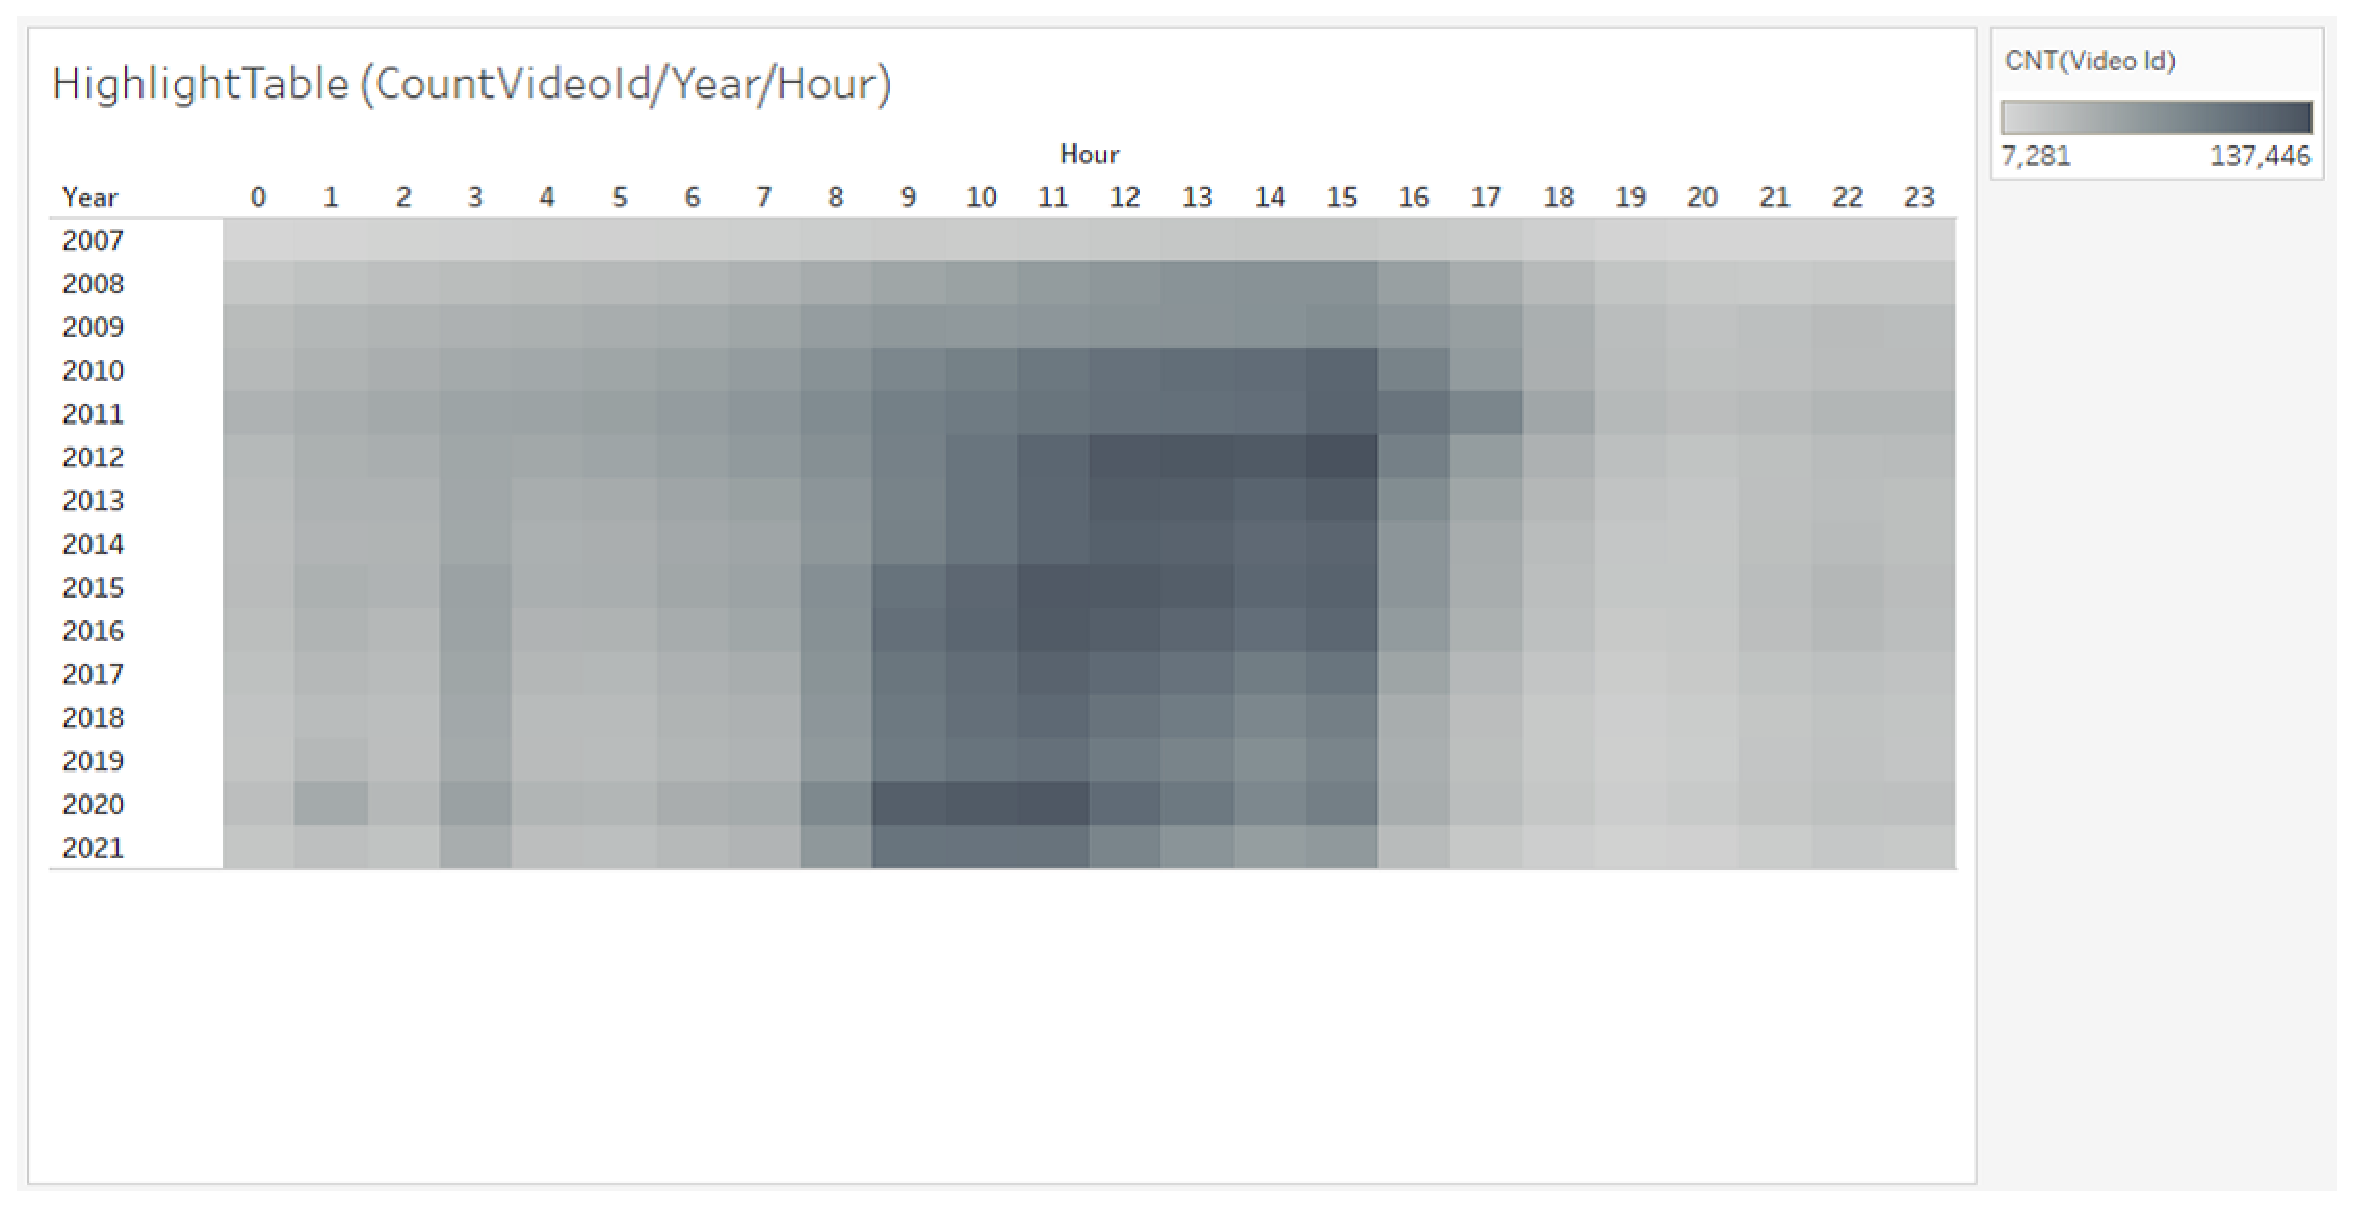
\includegraphics[width=\columnwidth]{./eps/HighlightTable_CountVideoId_YearHour.eps}
    \subcaption{Year/Hour}\label{fig:highlighttable_countvideoid_weekday_hour}
  \end{minipage}
  %
  \begin{minipage}[b]{0.49\columnwidth}
    \centering
    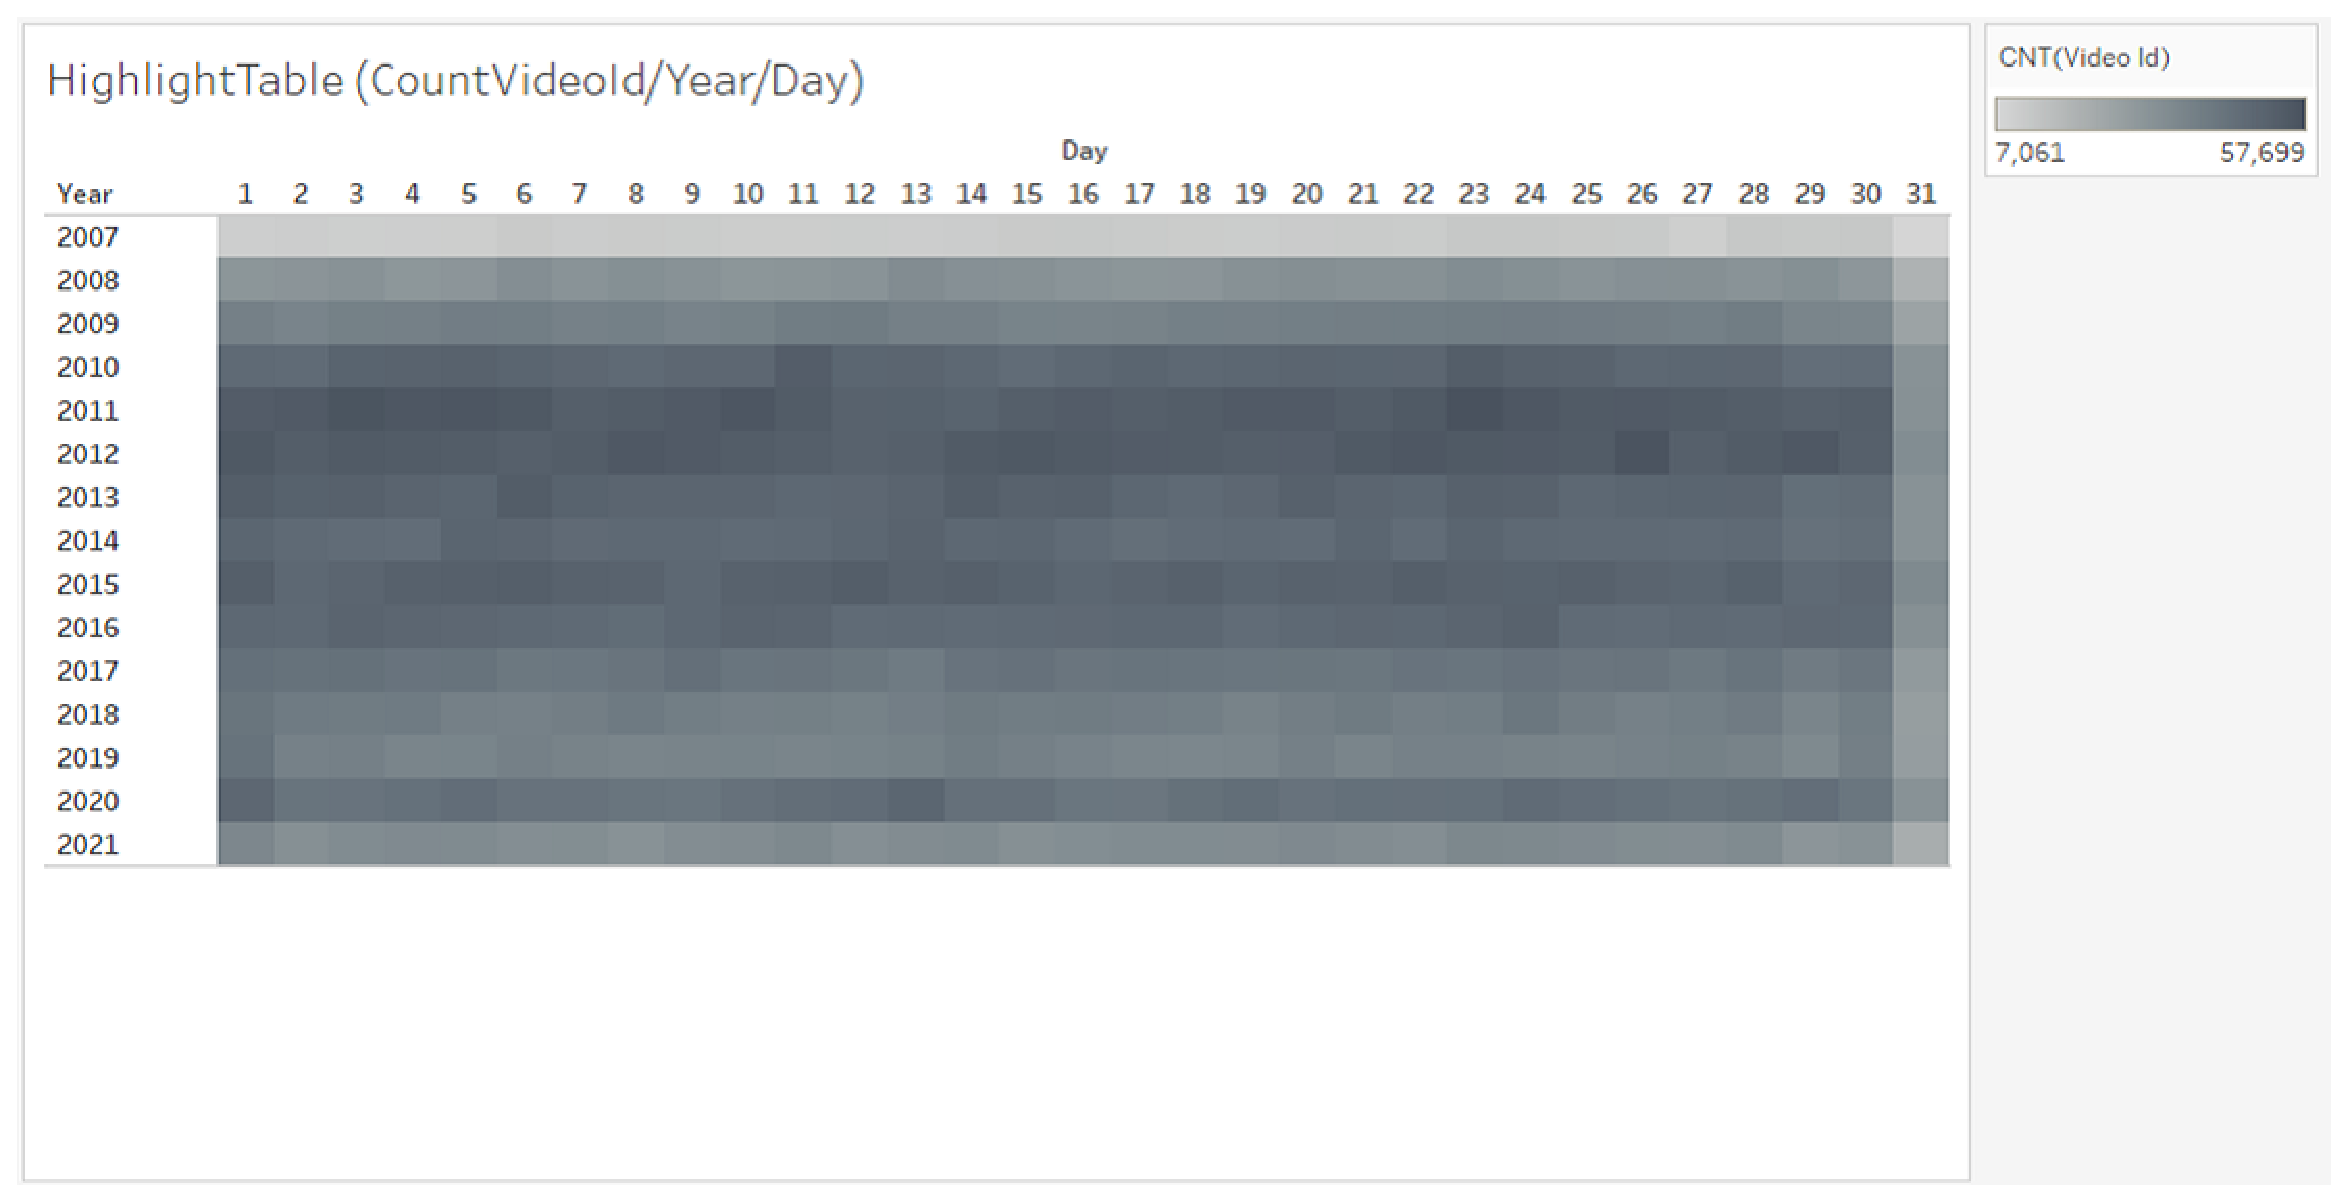
\includegraphics[width=\columnwidth]{./eps/HighlightTable_CountVideoId_YearDay.eps}
    \subcaption{Year/Day}\label{fig:highlighttable_countvideoid_weekday_day}
  \end{minipage}
  %
  \begin{minipage}[b]{0.49\columnwidth}
    \centering
    \hspace{-1.0zh}
    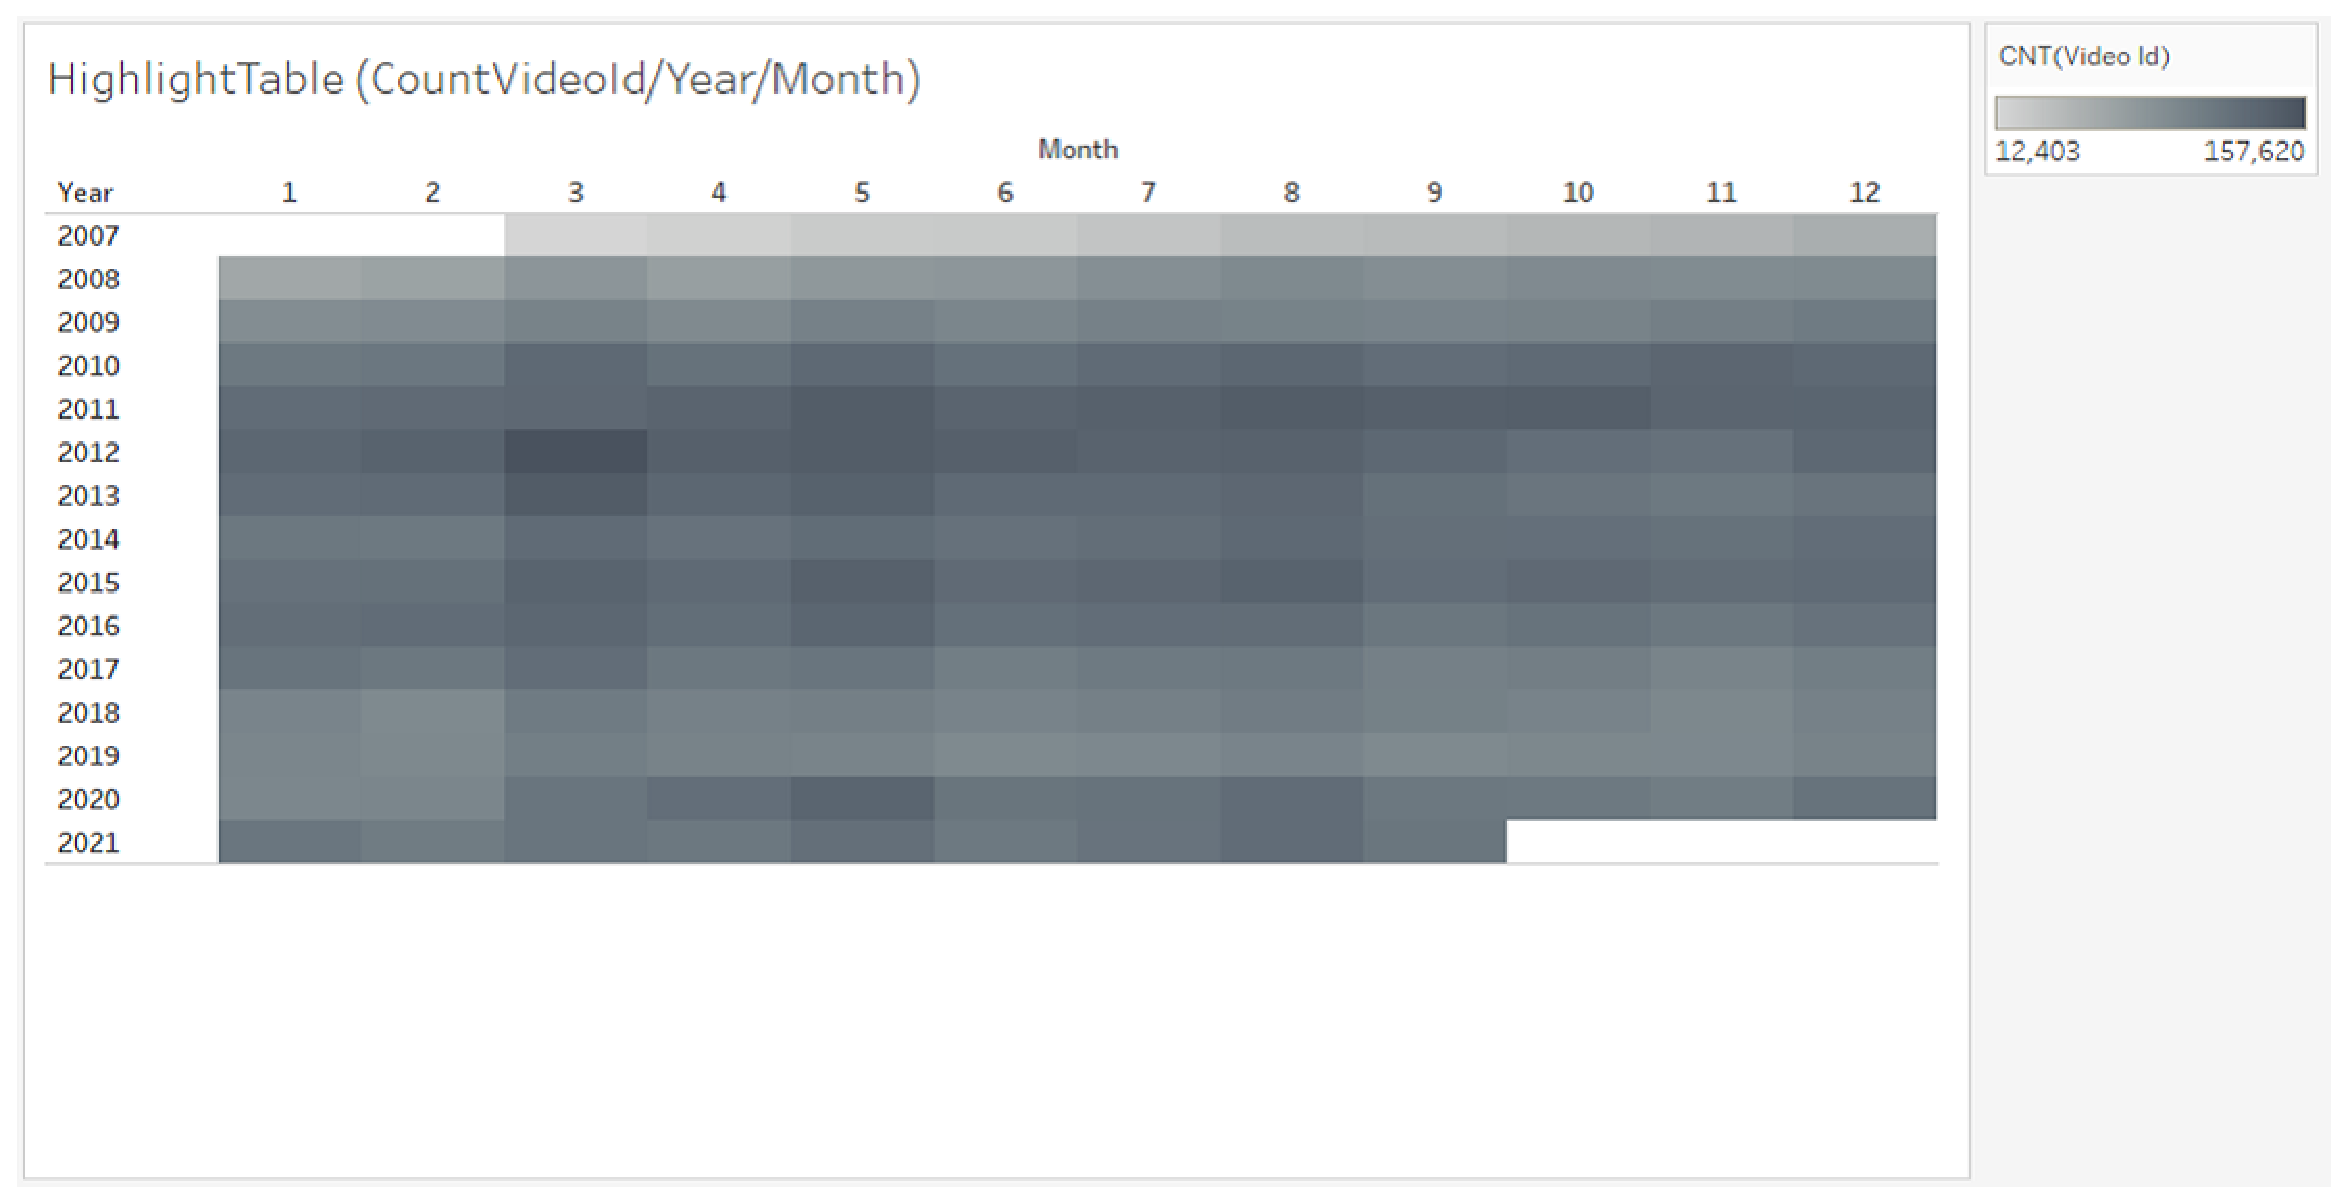
\includegraphics[width=\columnwidth]{./eps/HighlightTable_CountVideoId_YearMonth.eps}
    \subcaption{Year/Month}\label{fig:highlighttable_countvideoid_weekday_month}
  \end{minipage}
  %
  \begin{minipage}[b]{0.49\columnwidth}
    \centering
    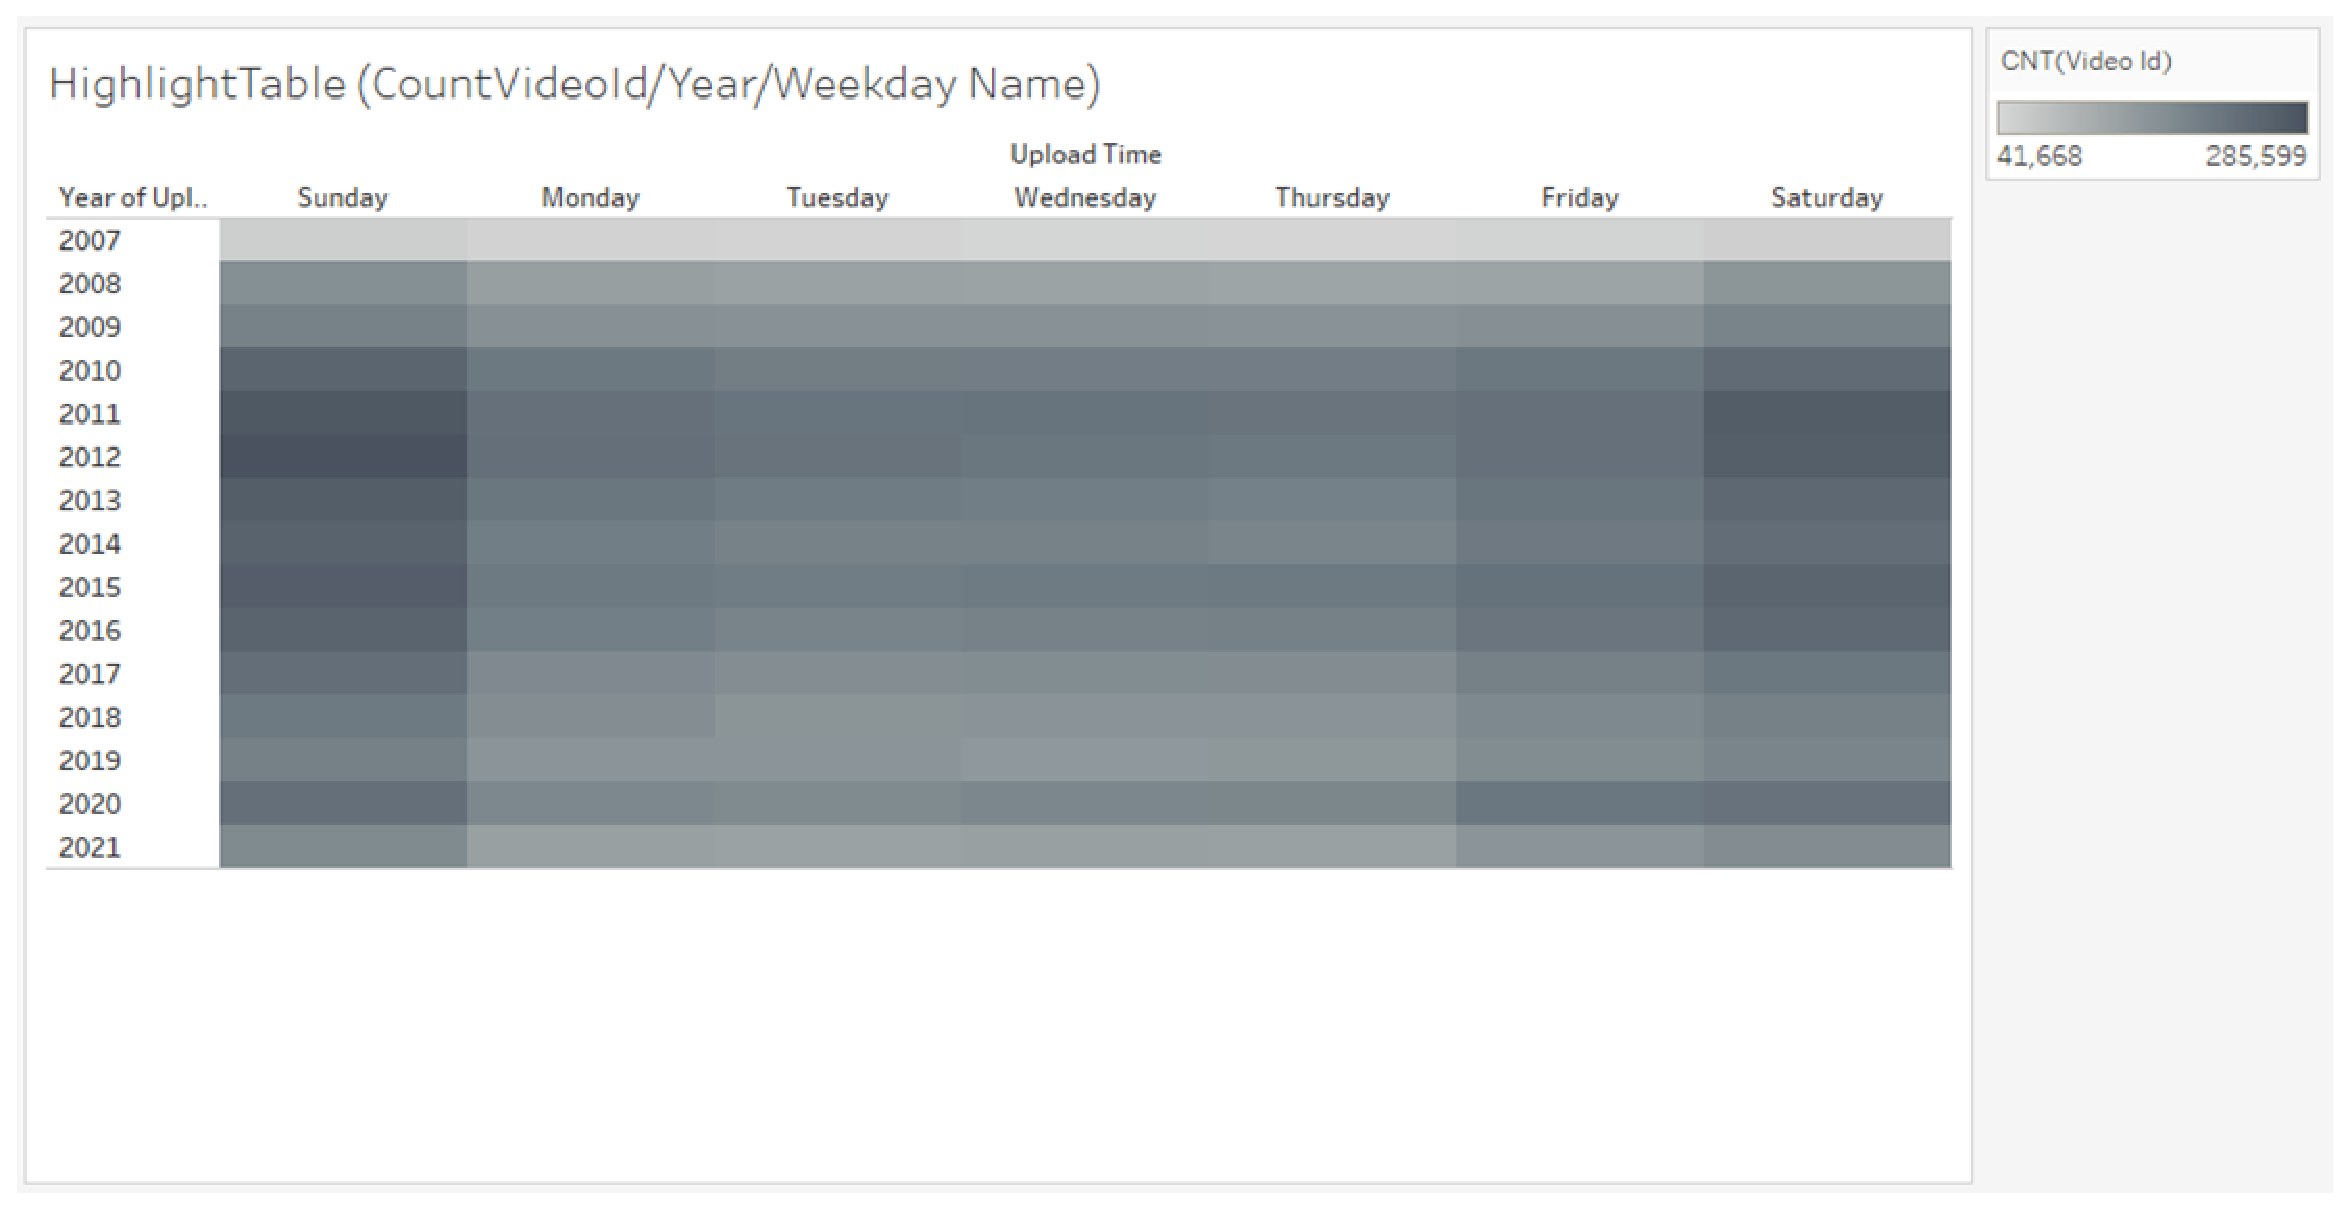
\includegraphics[width=\columnwidth]{./eps/HighlightTable_CountVideoId_YearWeekdayName.eps}
    \subcaption{Year/WeekdayName}\label{fig:highlighttable_countvideoid_weekday_year}
  \end{minipage}
  \caption{CountVideoId(1)}
  \label{fig:highlighttable_countvideoid_year}
\end{figure}
\vspace{-3.0zh}
\begin{figure}[h]
  \begin{minipage}[b]{0.49\columnwidth}
    \centering
    \hspace{-1.0zh}
    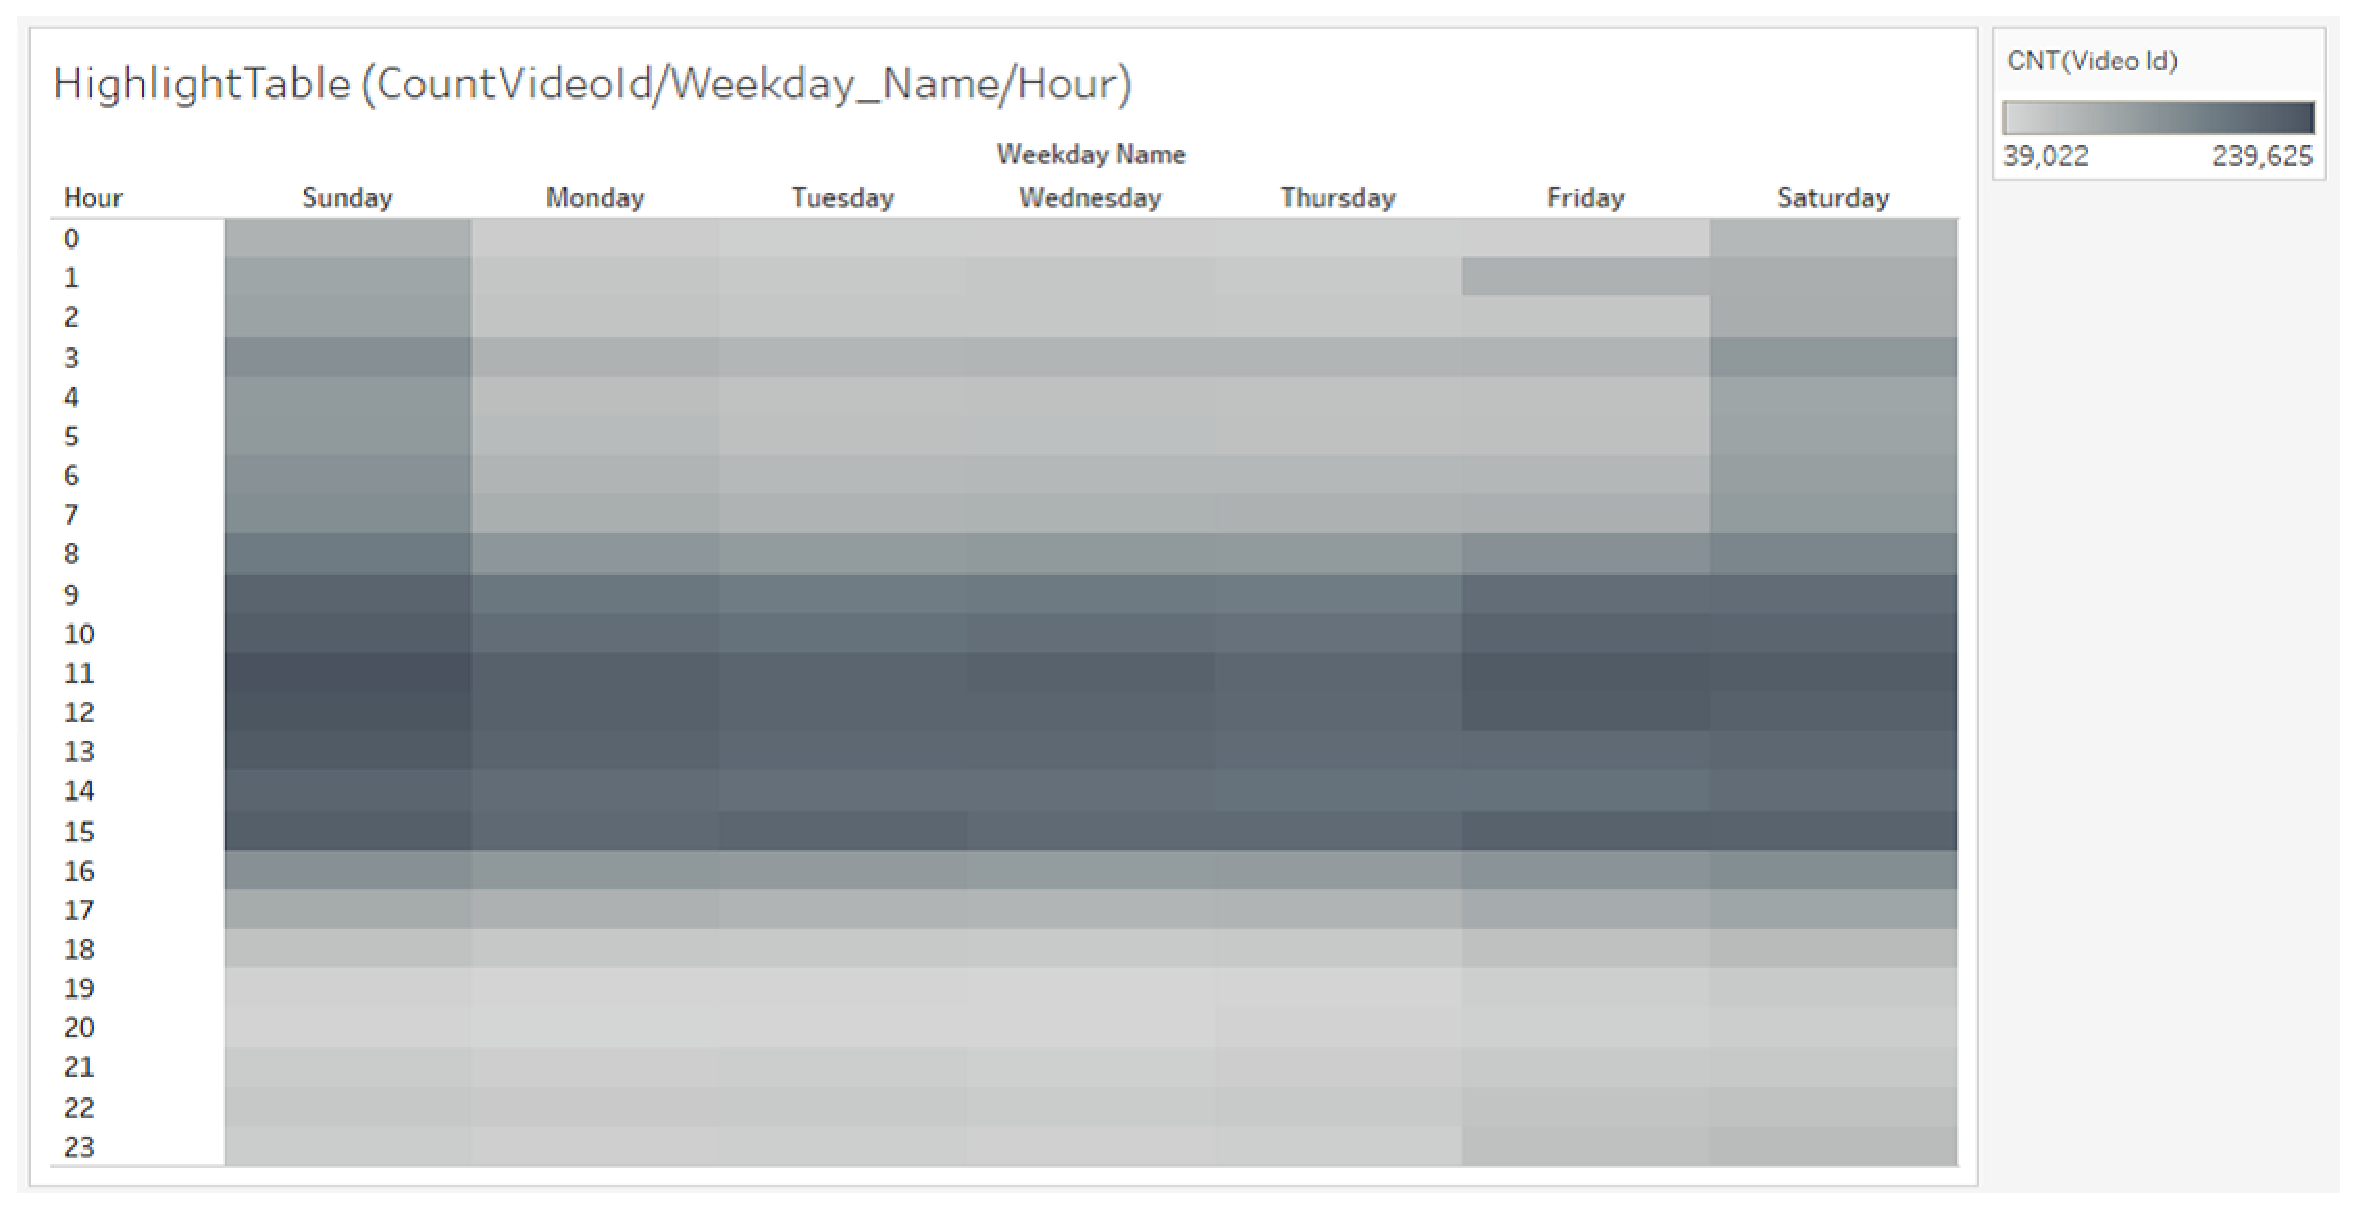
\includegraphics[width=\columnwidth]{./eps/HighlightTable_CountVideoId_WeekdayNameHour.eps}
    \subcaption{Hour/WeekdayName}\label{fig:highlighttable_countvideoid_weekday_hour}
  \end{minipage}
  %
  \begin{minipage}[b]{0.49\columnwidth}
    \centering
    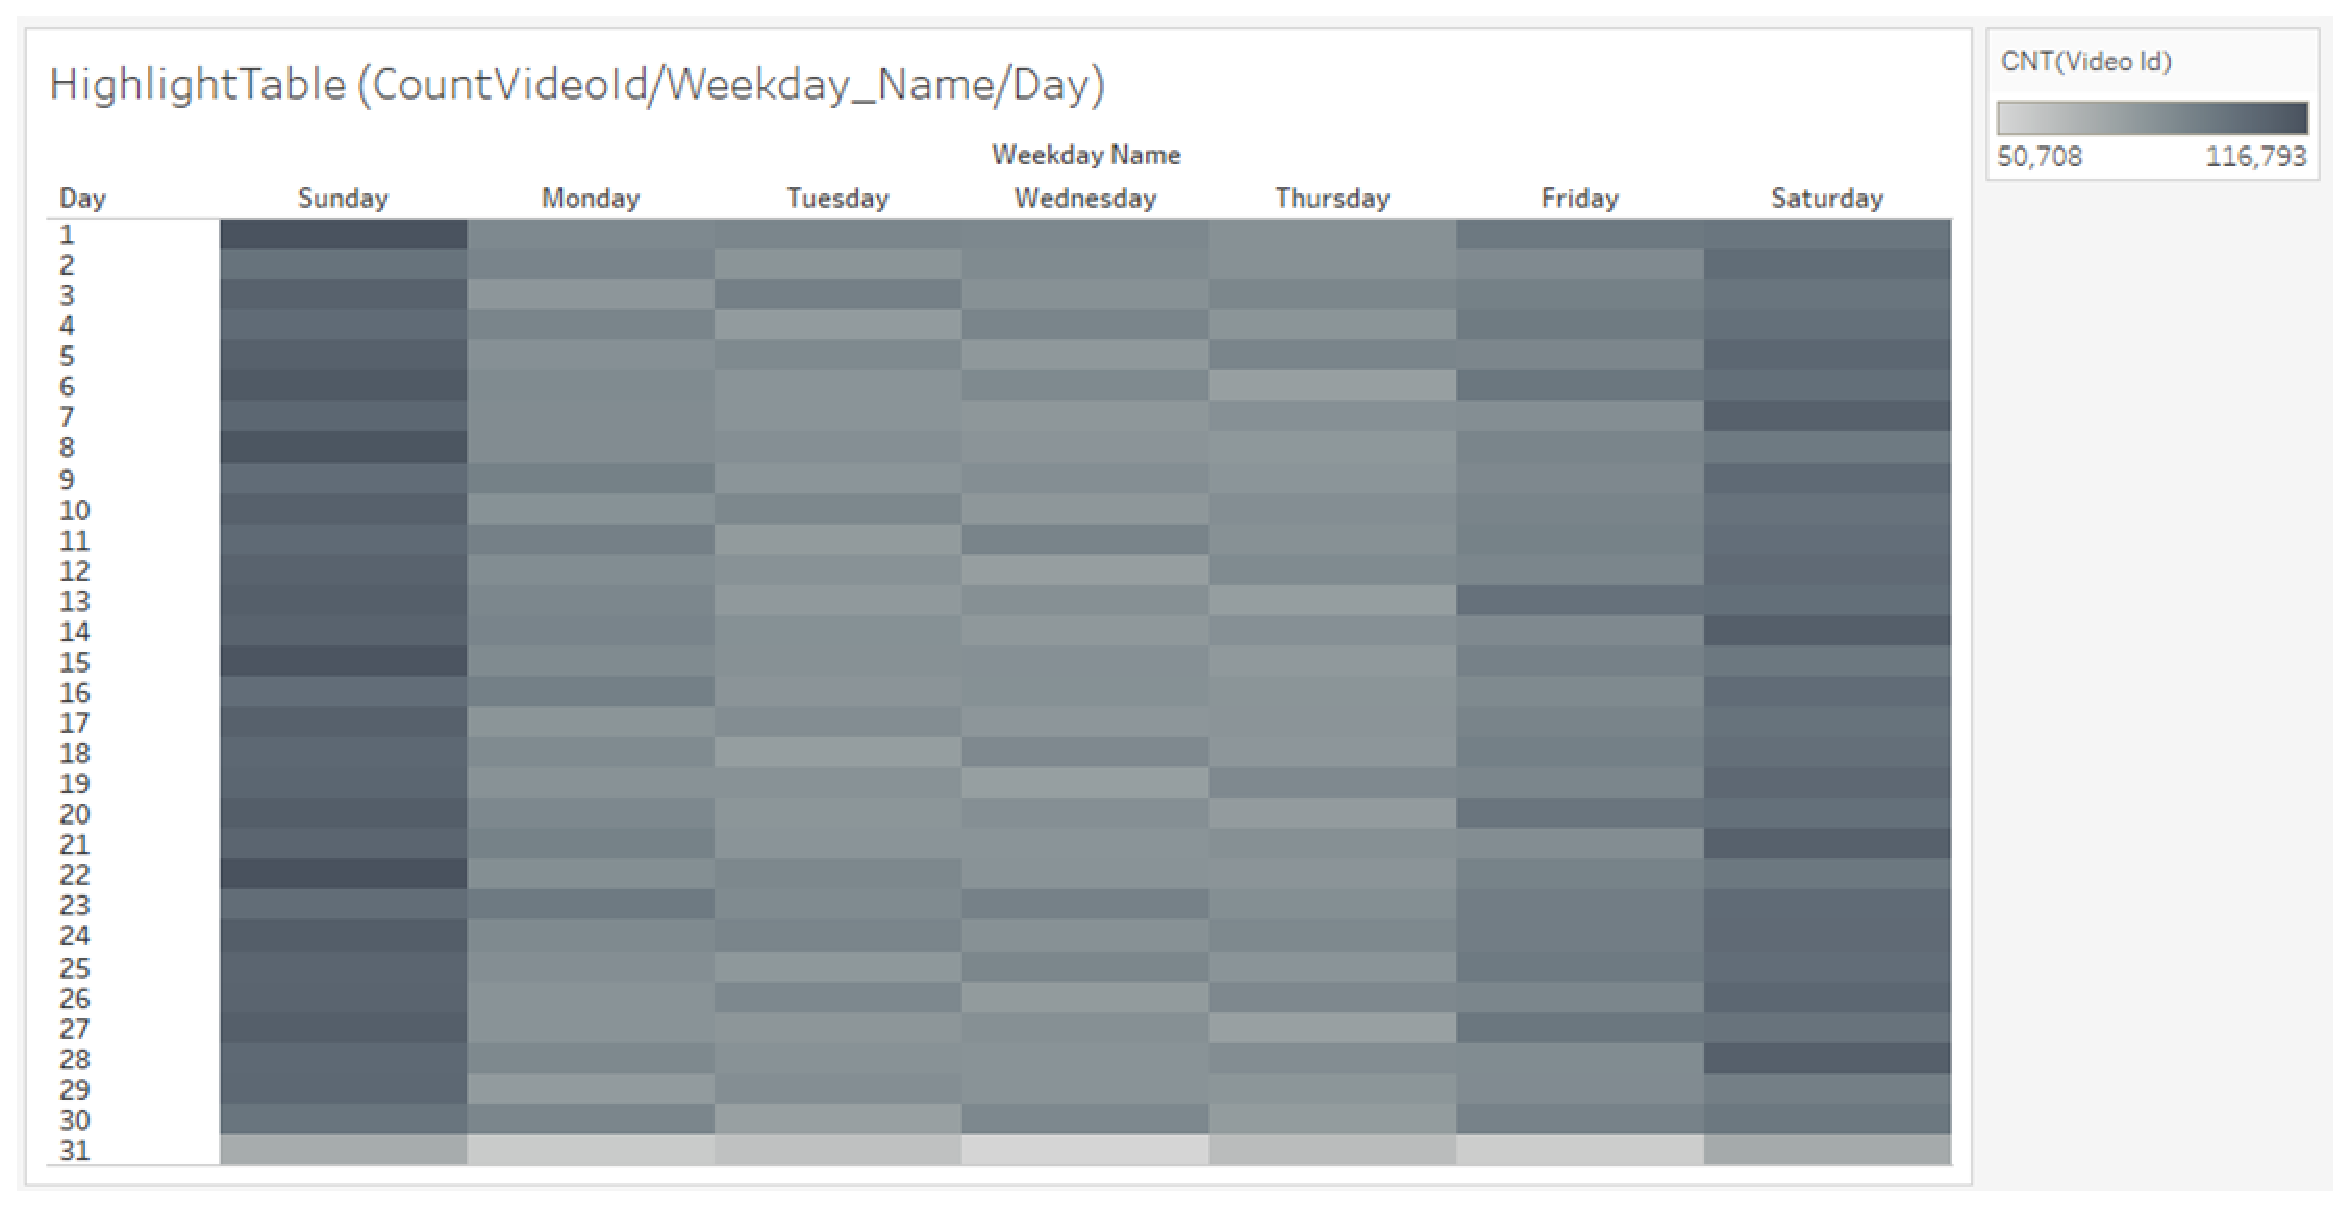
\includegraphics[width=\columnwidth]{./eps/HighlightTable_CountVideoId_WeekdayNameDay.eps}
    \subcaption{Day/WeekdayName}\label{fig:highlighttable_countvideoid_weekday_day}
  \end{minipage}
  %
  \begin{minipage}[b]{0.49\columnwidth}
    \centering
    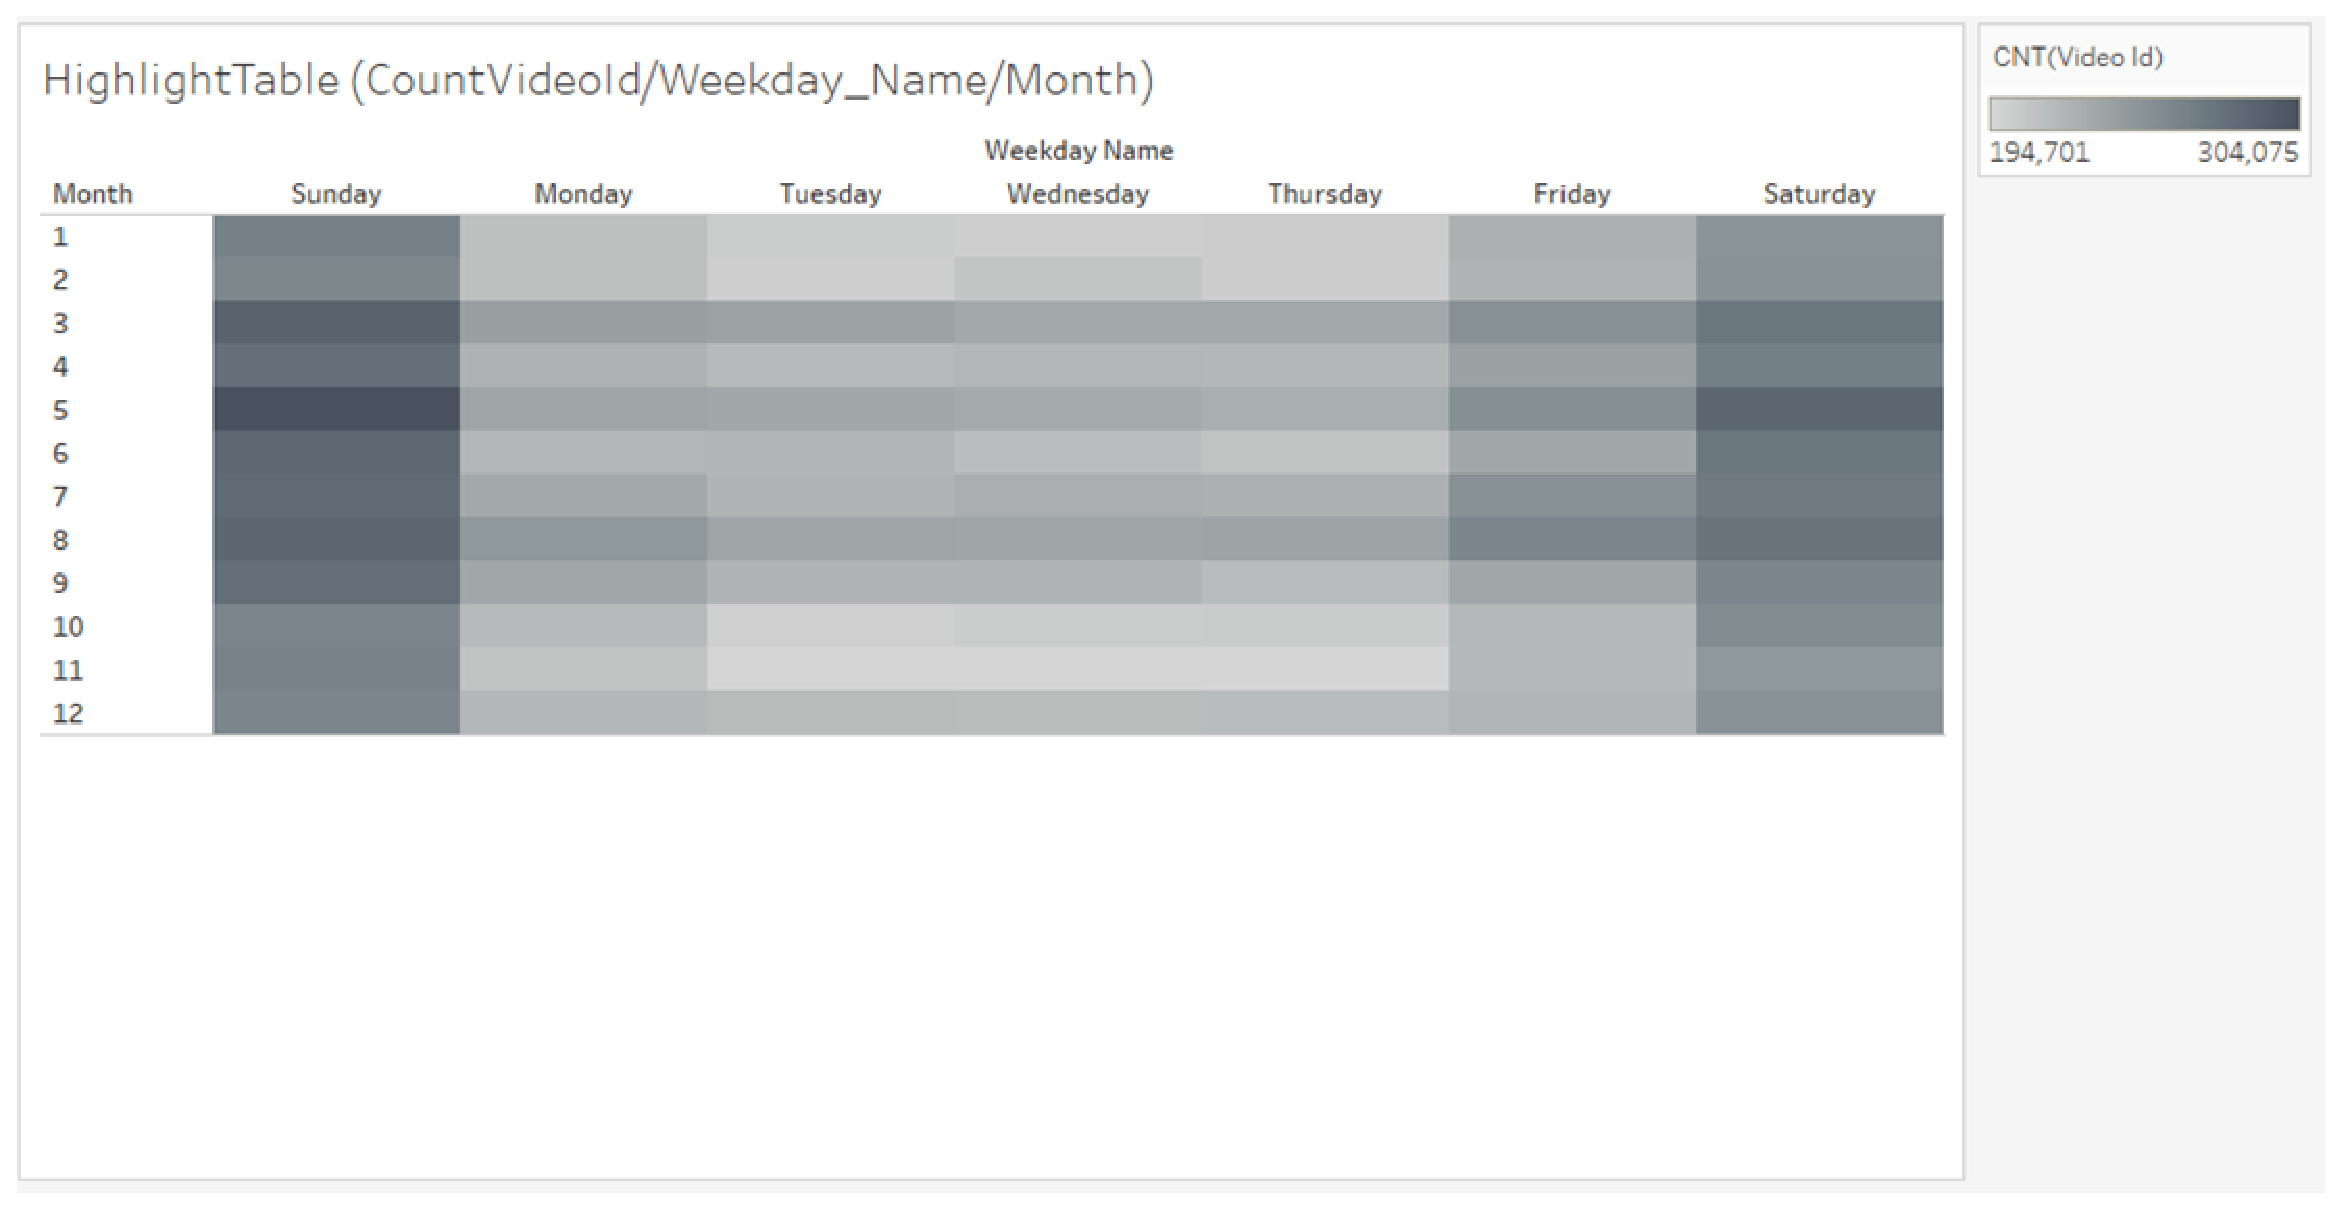
\includegraphics[width=\columnwidth]{./eps/HighlightTable_CountVideoId_WeekdayNameMonth.eps}
    \subcaption{Month/WeekdayName}\label{fig:highlighttable_countvideoid_weekday_month}
  \end{minipage}
  %
  \begin{minipage}[b]{0.49\columnwidth}
    \centering
    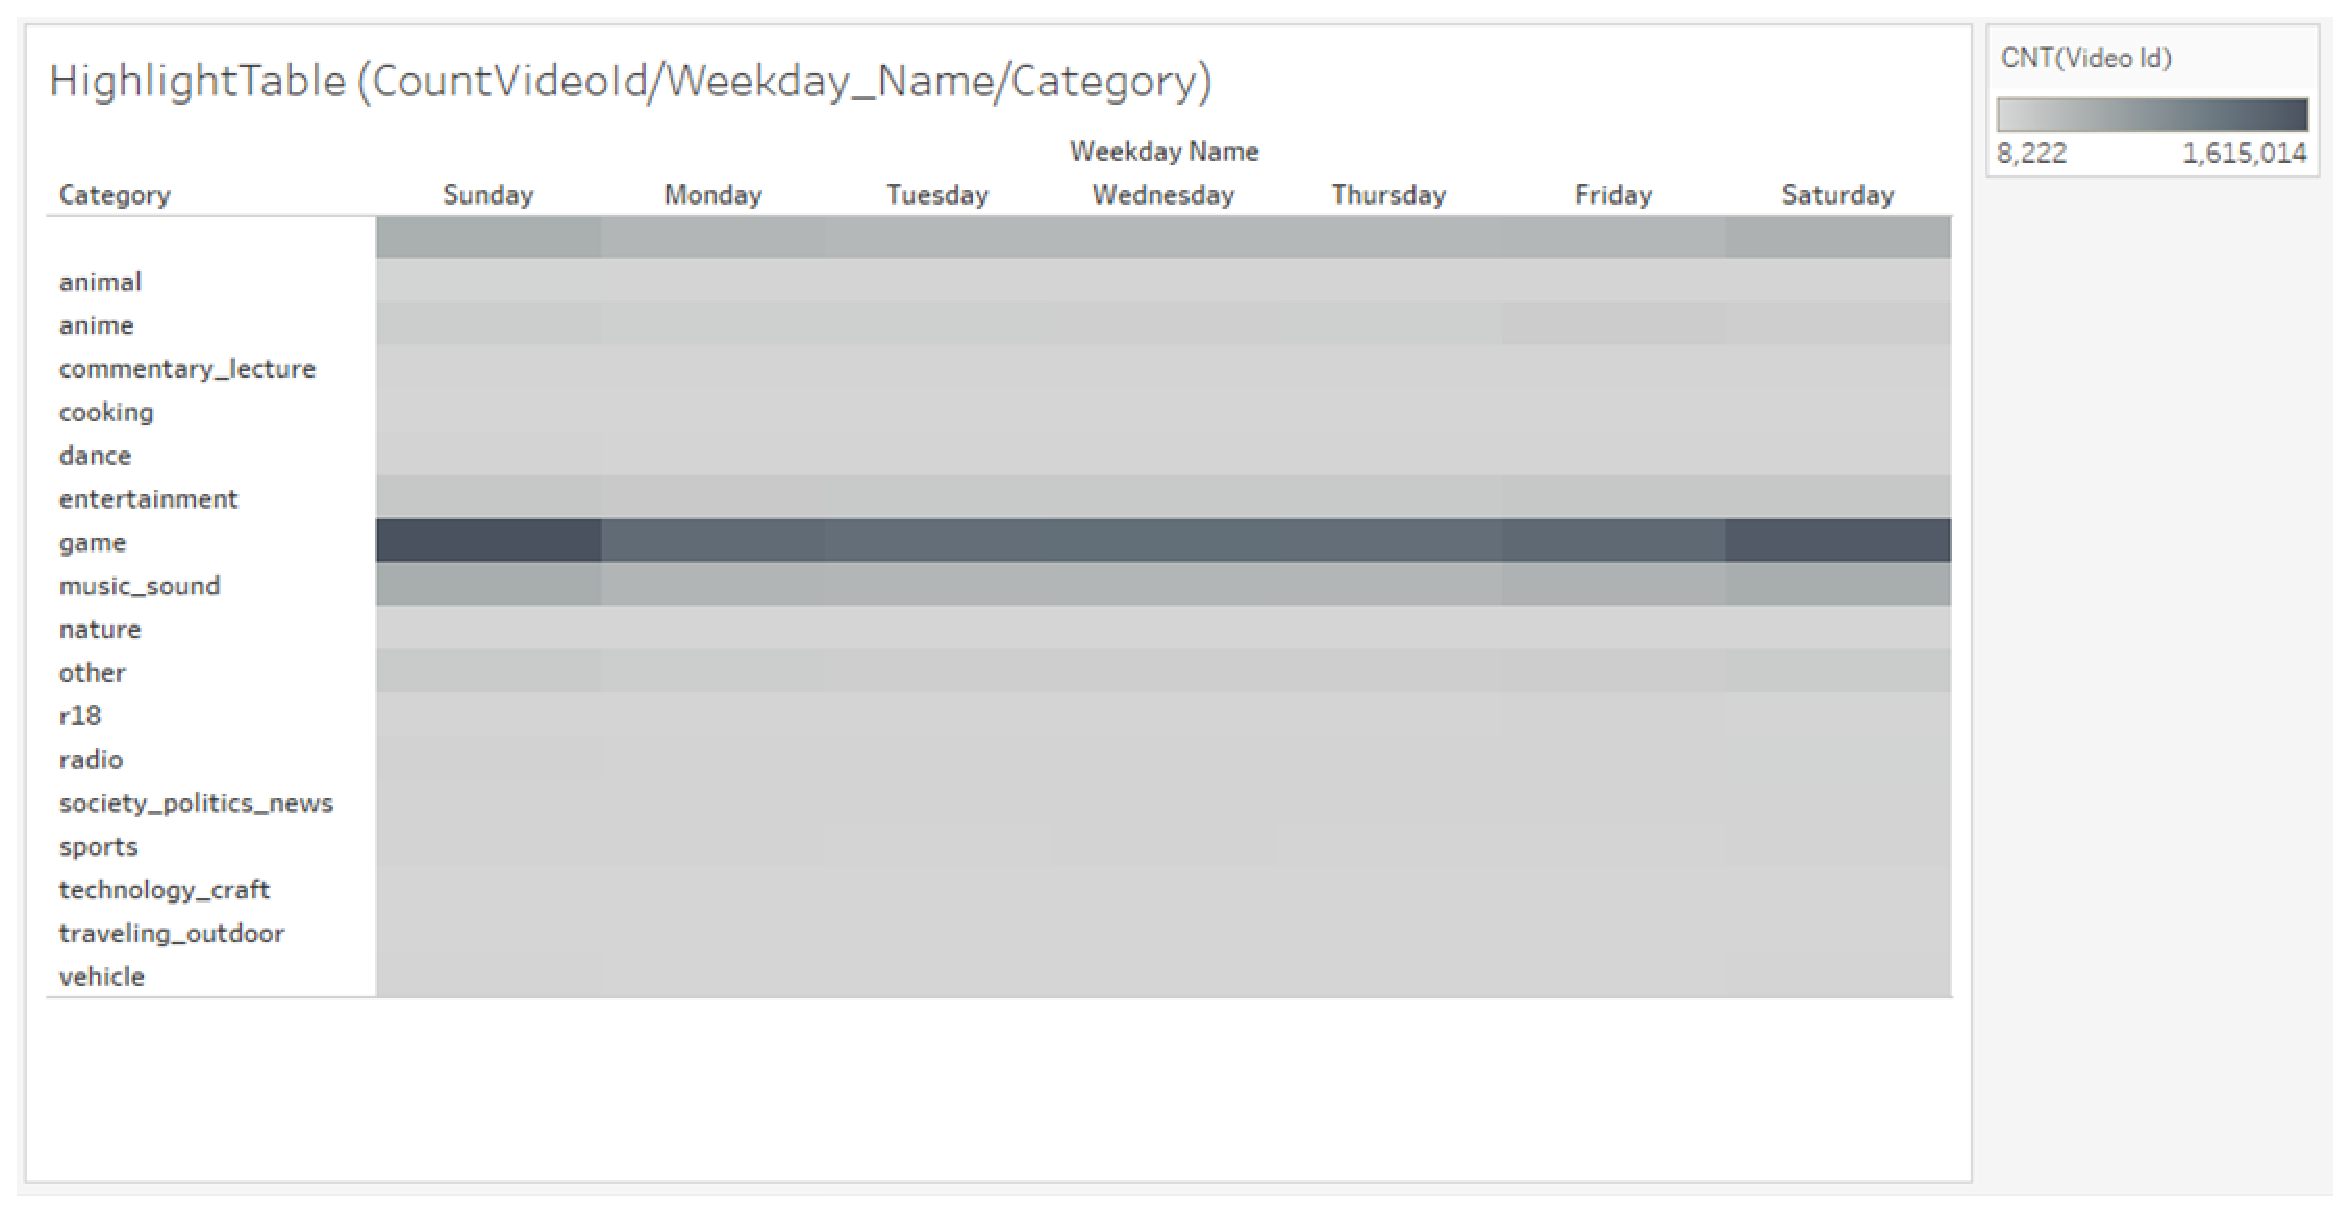
\includegraphics[width=\columnwidth]{./eps/HighlightTable_CountVideoId_WeekdayNameCategory.eps}
    \subcaption{Category/WeekdayName}\label{fig:highlighttable_countvideoid_weekday_category}
  \end{minipage}
  \caption{CountVideoId(2)}
  \label{fig:highlighttable_countvideoid_weekday}
\end{figure}
\vspace{-2.0zh}

図\ref{fig:highlighttable_countvideoid_weekday_hour}から
図\ref{fig:highlighttable_countvideoid_weekday_year}の結果について考察する.
%
年と時間の集計した図\ref{fig:highlighttable_countvideoid_weekday_hour}では,
朝の8時から夕方17時までの間の投稿が多く,投稿年が進むにつれて投稿時間は早まる傾向にあった.
%
年と日で集計した図\ref{fig:highlighttable_countvideoid_weekday_day}では,
各年単位で集計では,月末や月初など時期による違いは見受けられない.
%
年と月で集計した図\ref{fig:highlighttable_countvideoid_weekday_month}では,
3月や8月については,他の月と比較してが投稿動画が多い.
%
年と曜日で集計した図\ref{fig:highlighttable_countvideoid_weekday_year}では,
土曜日と日曜日の投稿動画数が多い.
%
このことから,動画投稿の傾向や集中した時期を可視化することができたと言える.

また,図\ref{fig:highlighttable_countvideoid_weekday_hour}から
図\ref{fig:highlighttable_countvideoid_weekday_category}の結果について考察する.
%
時間と曜日で集計した図\ref{fig:highlighttable_countvideoid_weekday_hour}では,
9時から15時までの投稿が多く,金曜日の9時から12時の間が最も投稿が盛んである.
%
日と曜日で集計した図\ref{fig:highlighttable_countvideoid_weekday_day}では,
土曜日の朝8時に動画投稿が集中していた.
%
月と曜日で集計した図\ref{fig:highlighttable_countvideoid_weekday_month}では,
各月土曜日と日曜日に動画投稿が集中しており,3月や5月が顕著だった.
%
カテゴリと曜日で集計した図\ref{fig:highlighttable_countvideoid_weekday_category}では,
ゲームの投稿動画が多いことが明らかである.
%
このことから,日や月では,曜日特有の投稿状況を可視化することができた.

\newpage

\subsection{HighlightTable分析 - WatchNum}

閲覧数を集計値として,可視化した結果を図\ref{fig:highlighttable_watchnum_year}および
図\ref{fig:highlighttable_watchnum_weekdayname}に示す.
%
図\ref{fig:highlighttable_watchnum_year}は縦軸が年であり,
横軸は時間,日,月,曜日の単位で集計している.
図\ref{fig:highlighttable_watchnum_weekdayname}は横軸が曜日であり,
縦軸は時間,日,月,カテゴリで集計している.

\vspace{-1.5zh}
\begin{figure}[h]
  \begin{minipage}[b]{0.49\columnwidth}
    \centering
    \hspace{-1.0zh}
    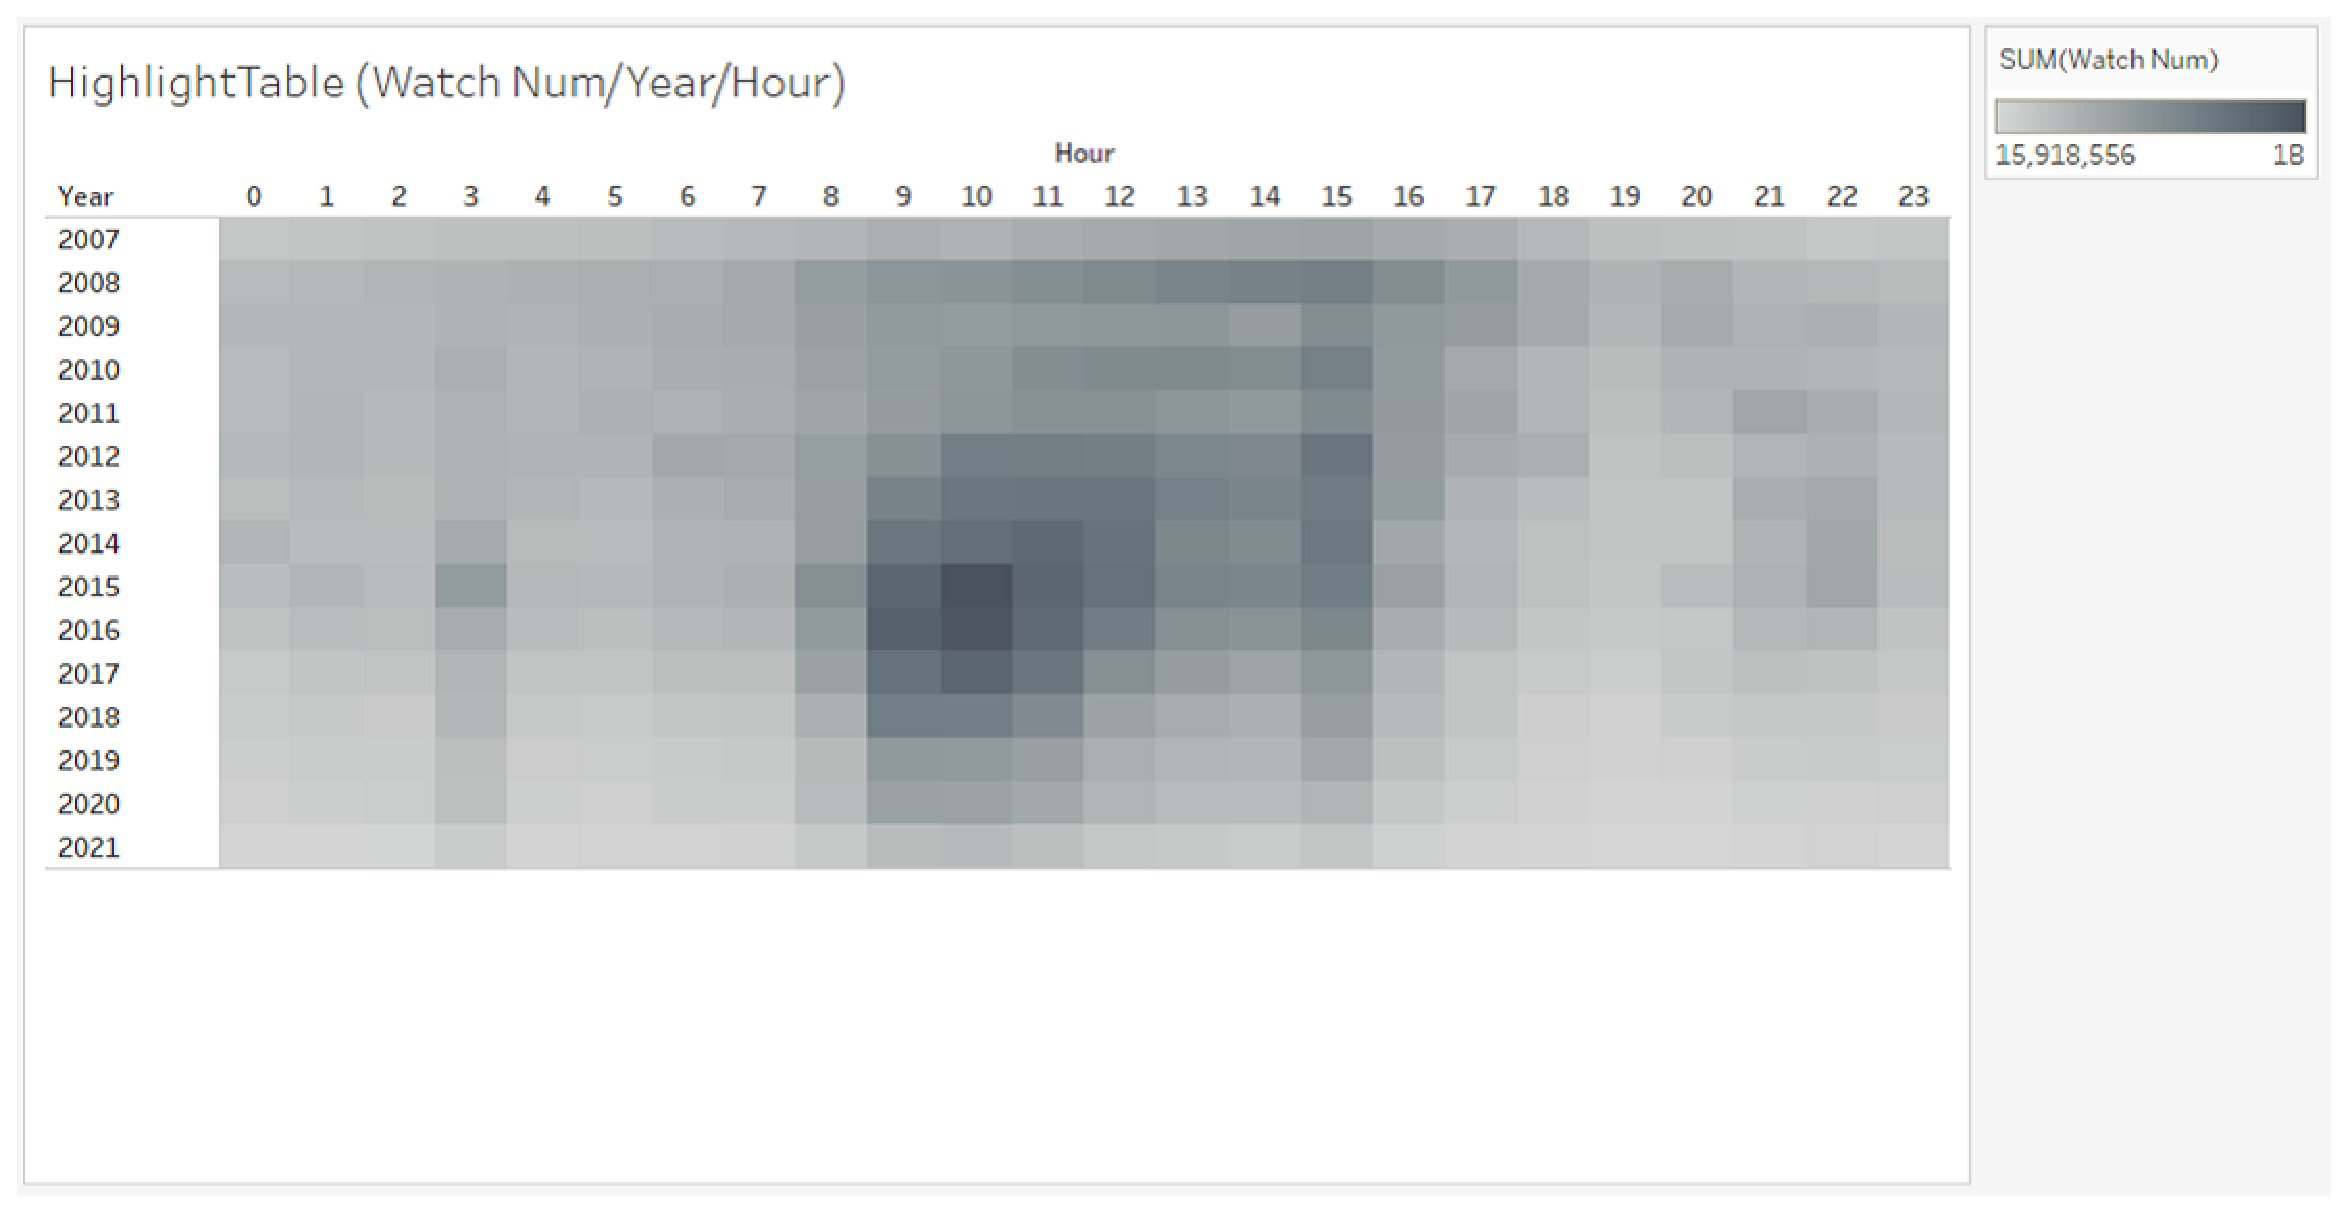
\includegraphics[width=\columnwidth]{./eps/HighlightTable_WatchNum_YearHour.eps}
    \subcaption{Year/Hour}\label{fig:highlighttable_watchnum_year_hour}
  \end{minipage}
  %
  \begin{minipage}[b]{0.49\columnwidth}
    \centering
    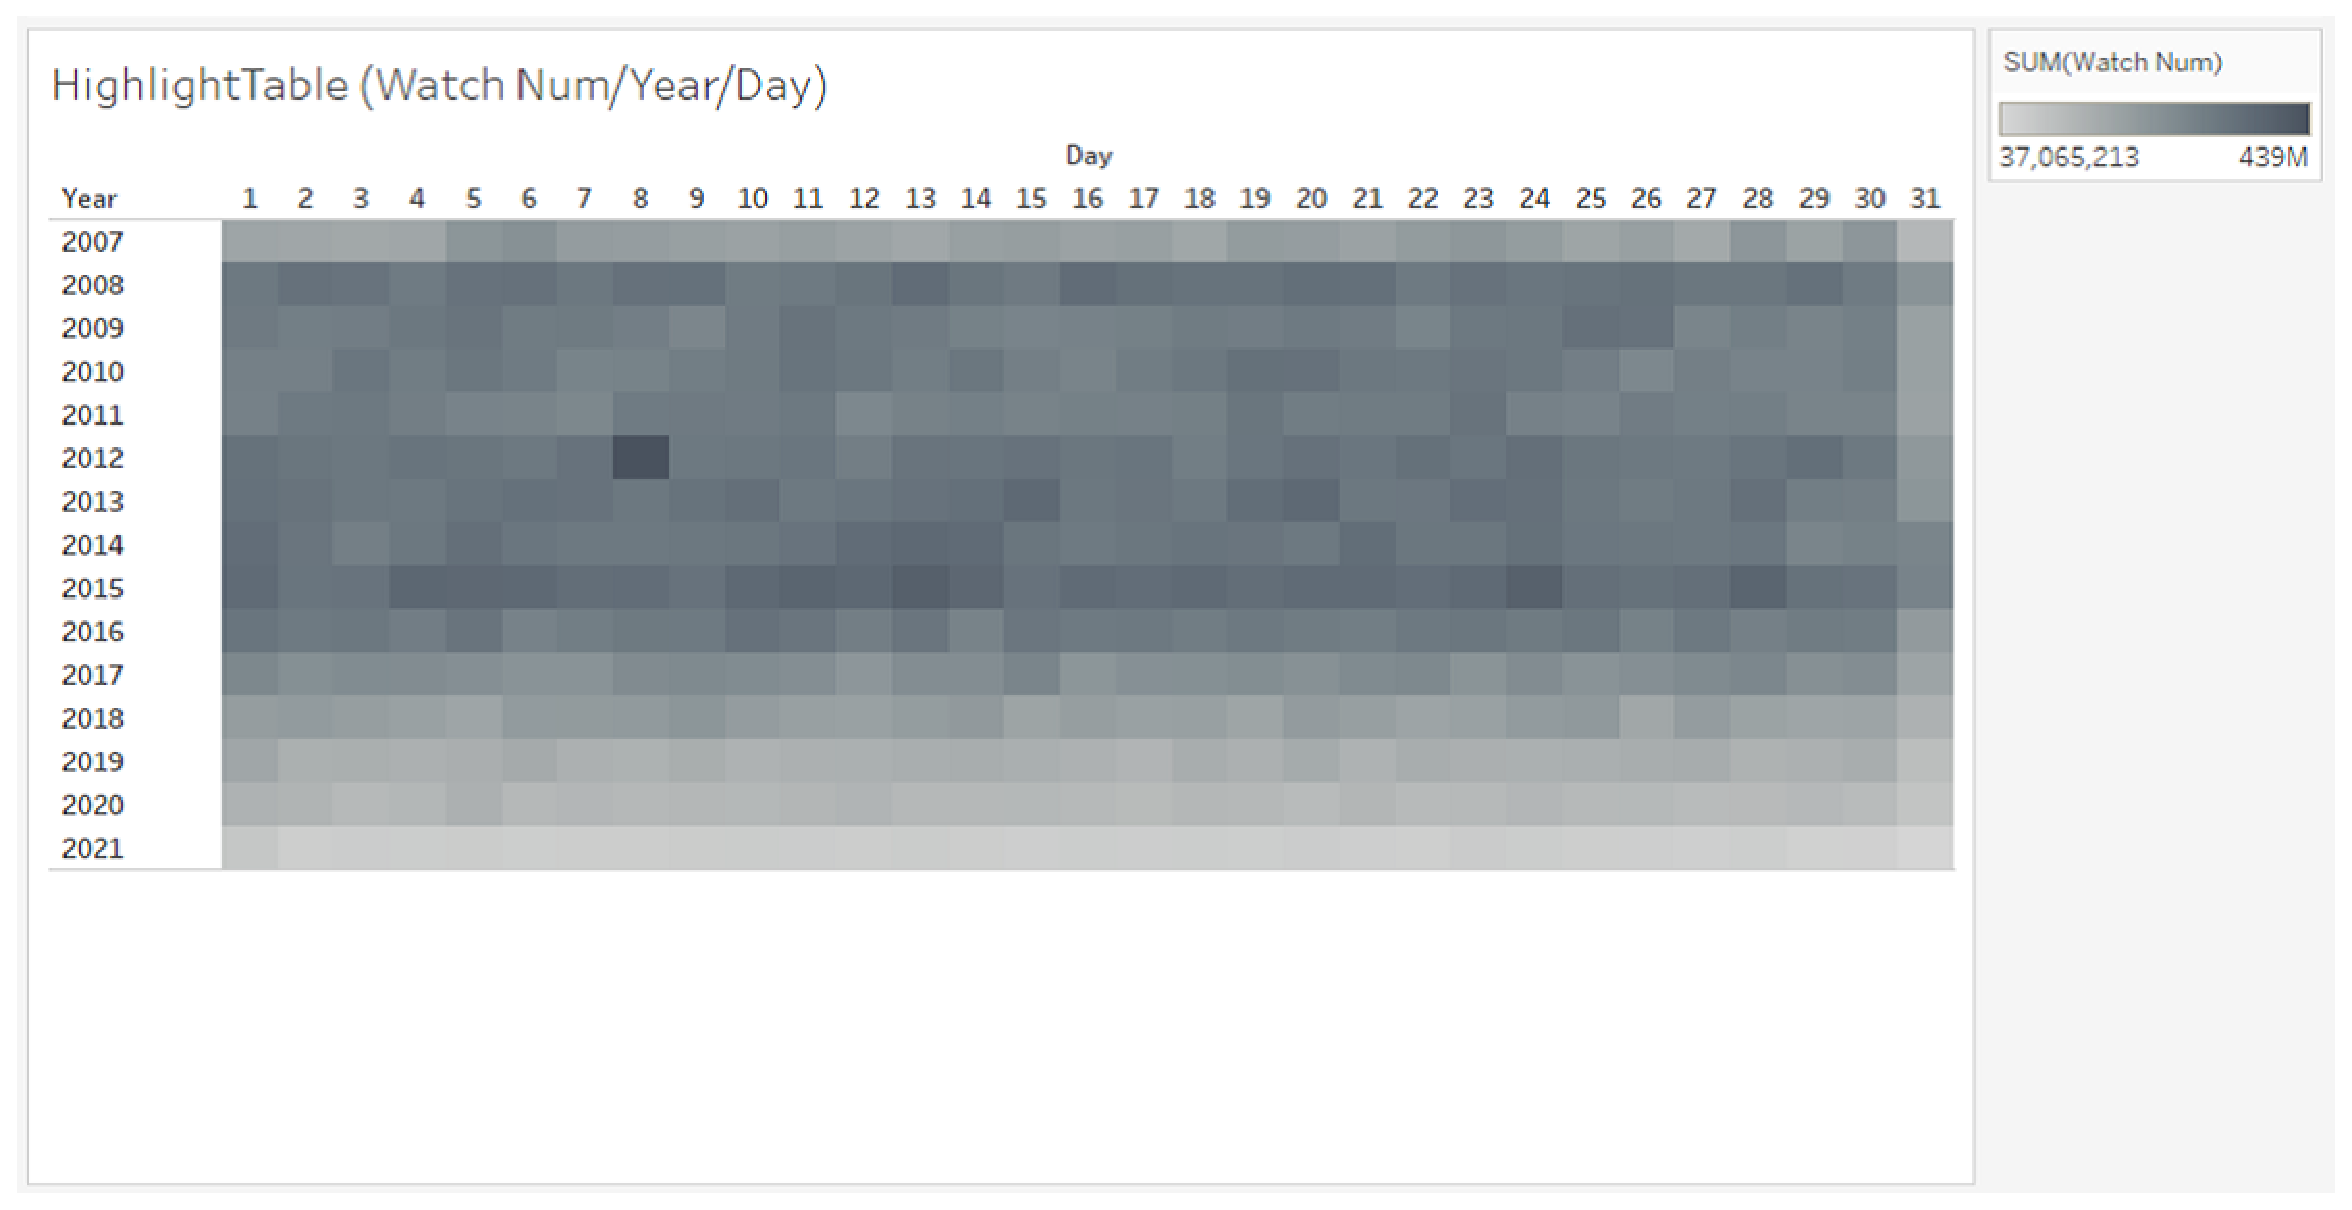
\includegraphics[width=\columnwidth]{./eps/HighlightTable_WatchNum_YearDay.eps}
    \subcaption{Year/Day}\label{fig:highlighttable_watchnum_year_day}
  \end{minipage}
  %
  \begin{minipage}[b]{0.49\columnwidth}
    \centering
    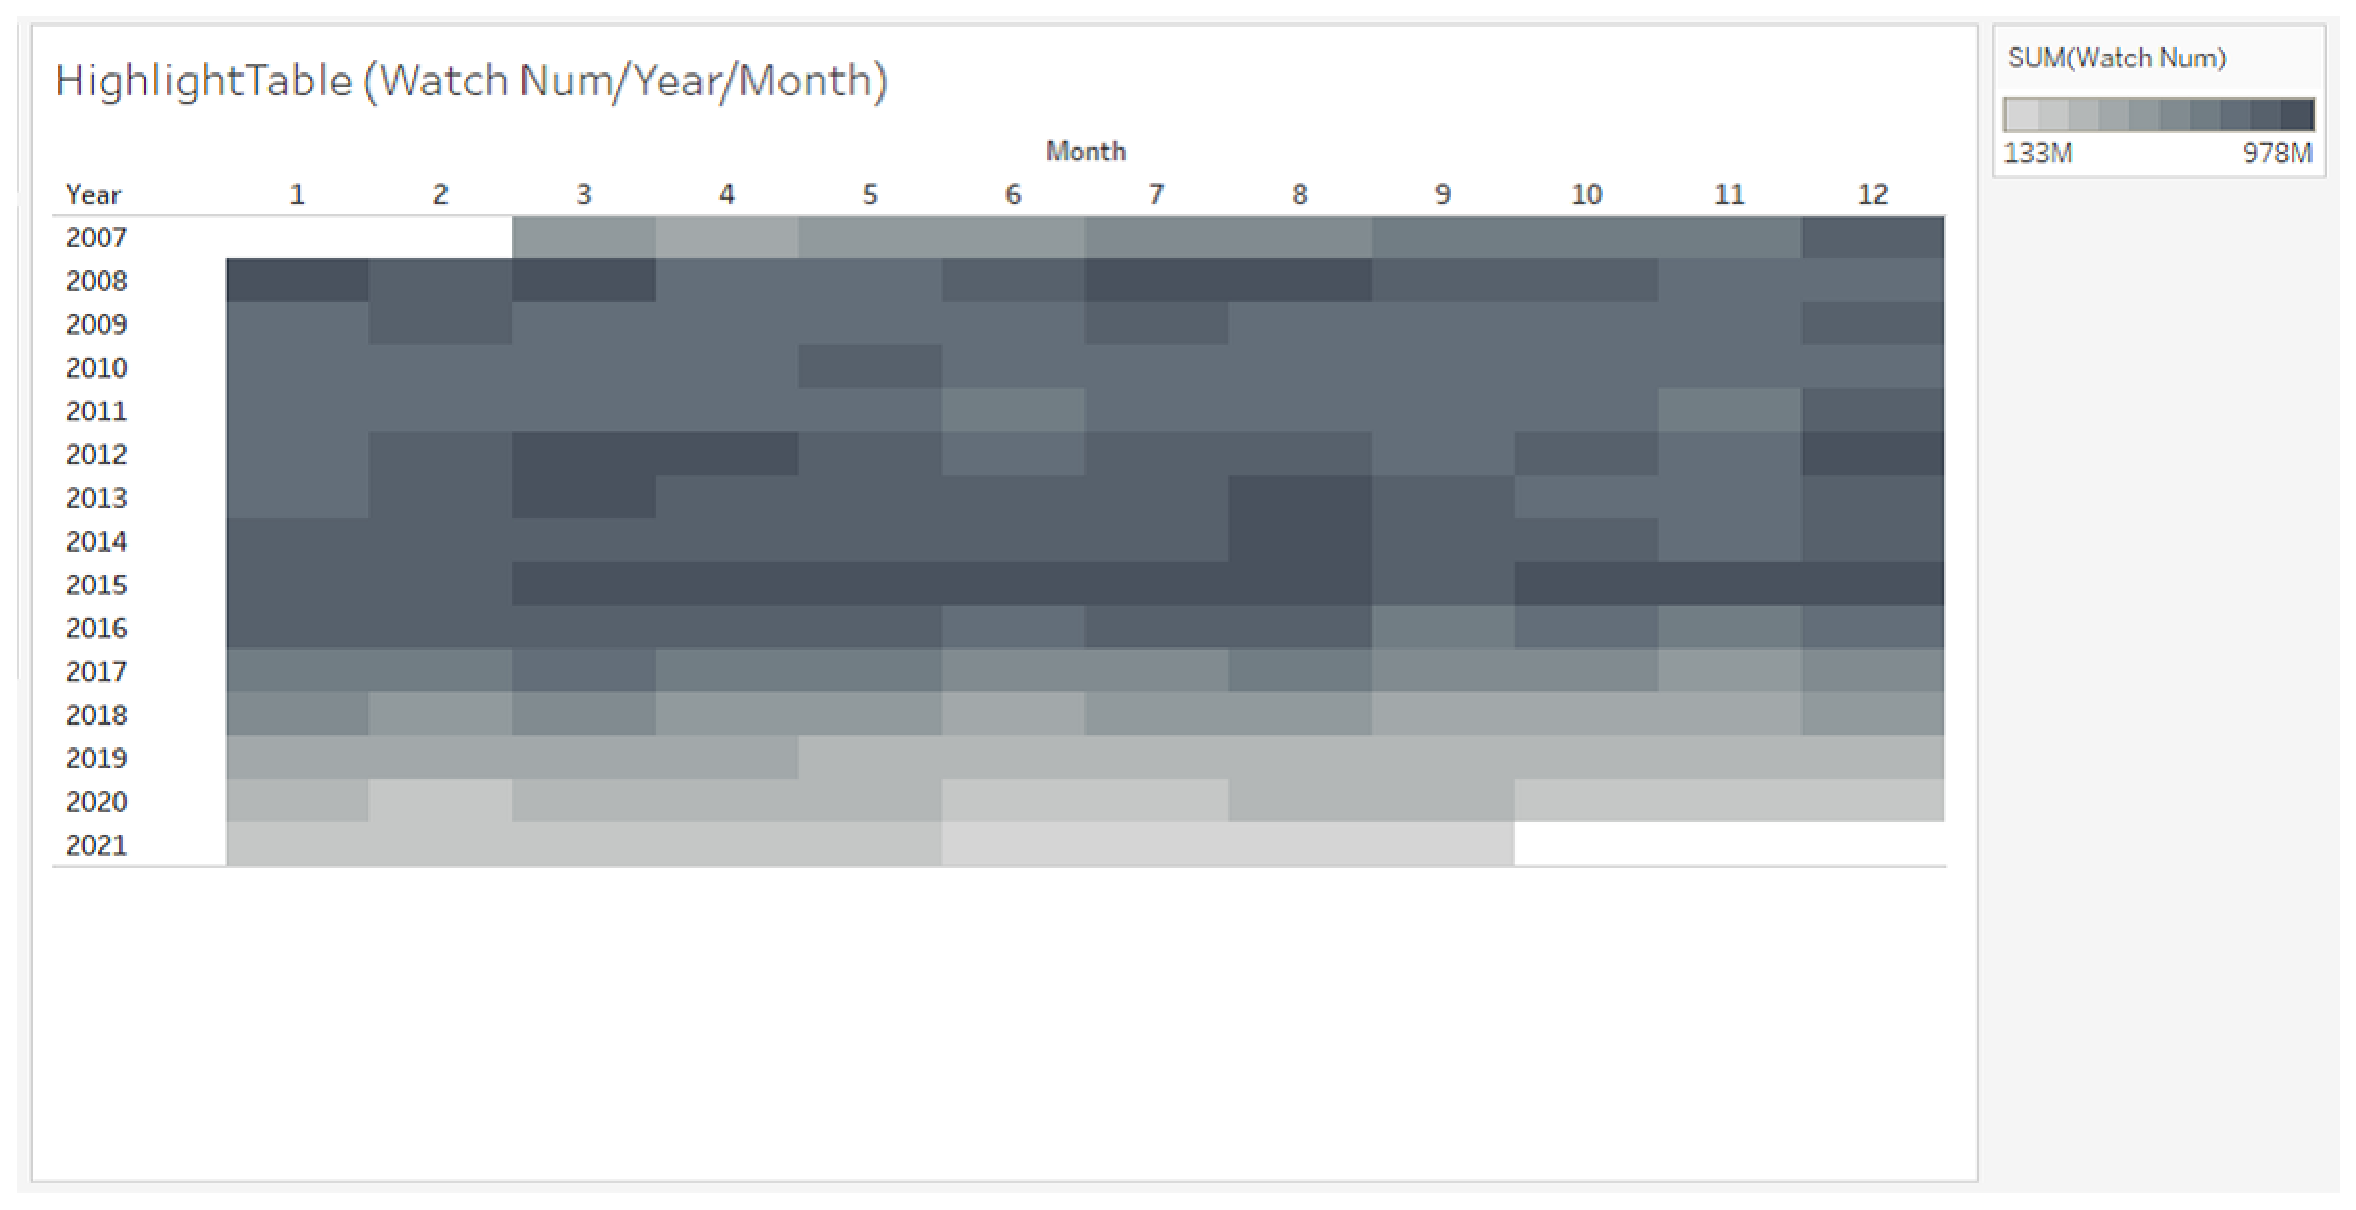
\includegraphics[width=\columnwidth]{./eps/HighlightTable_WatchNum_YearMonth.eps}
    \subcaption{Year/Month}\label{fig:highlighttable_watchnum_year_month}
  \end{minipage}
  %
  \begin{minipage}[b]{0.49\columnwidth}
    \centering
    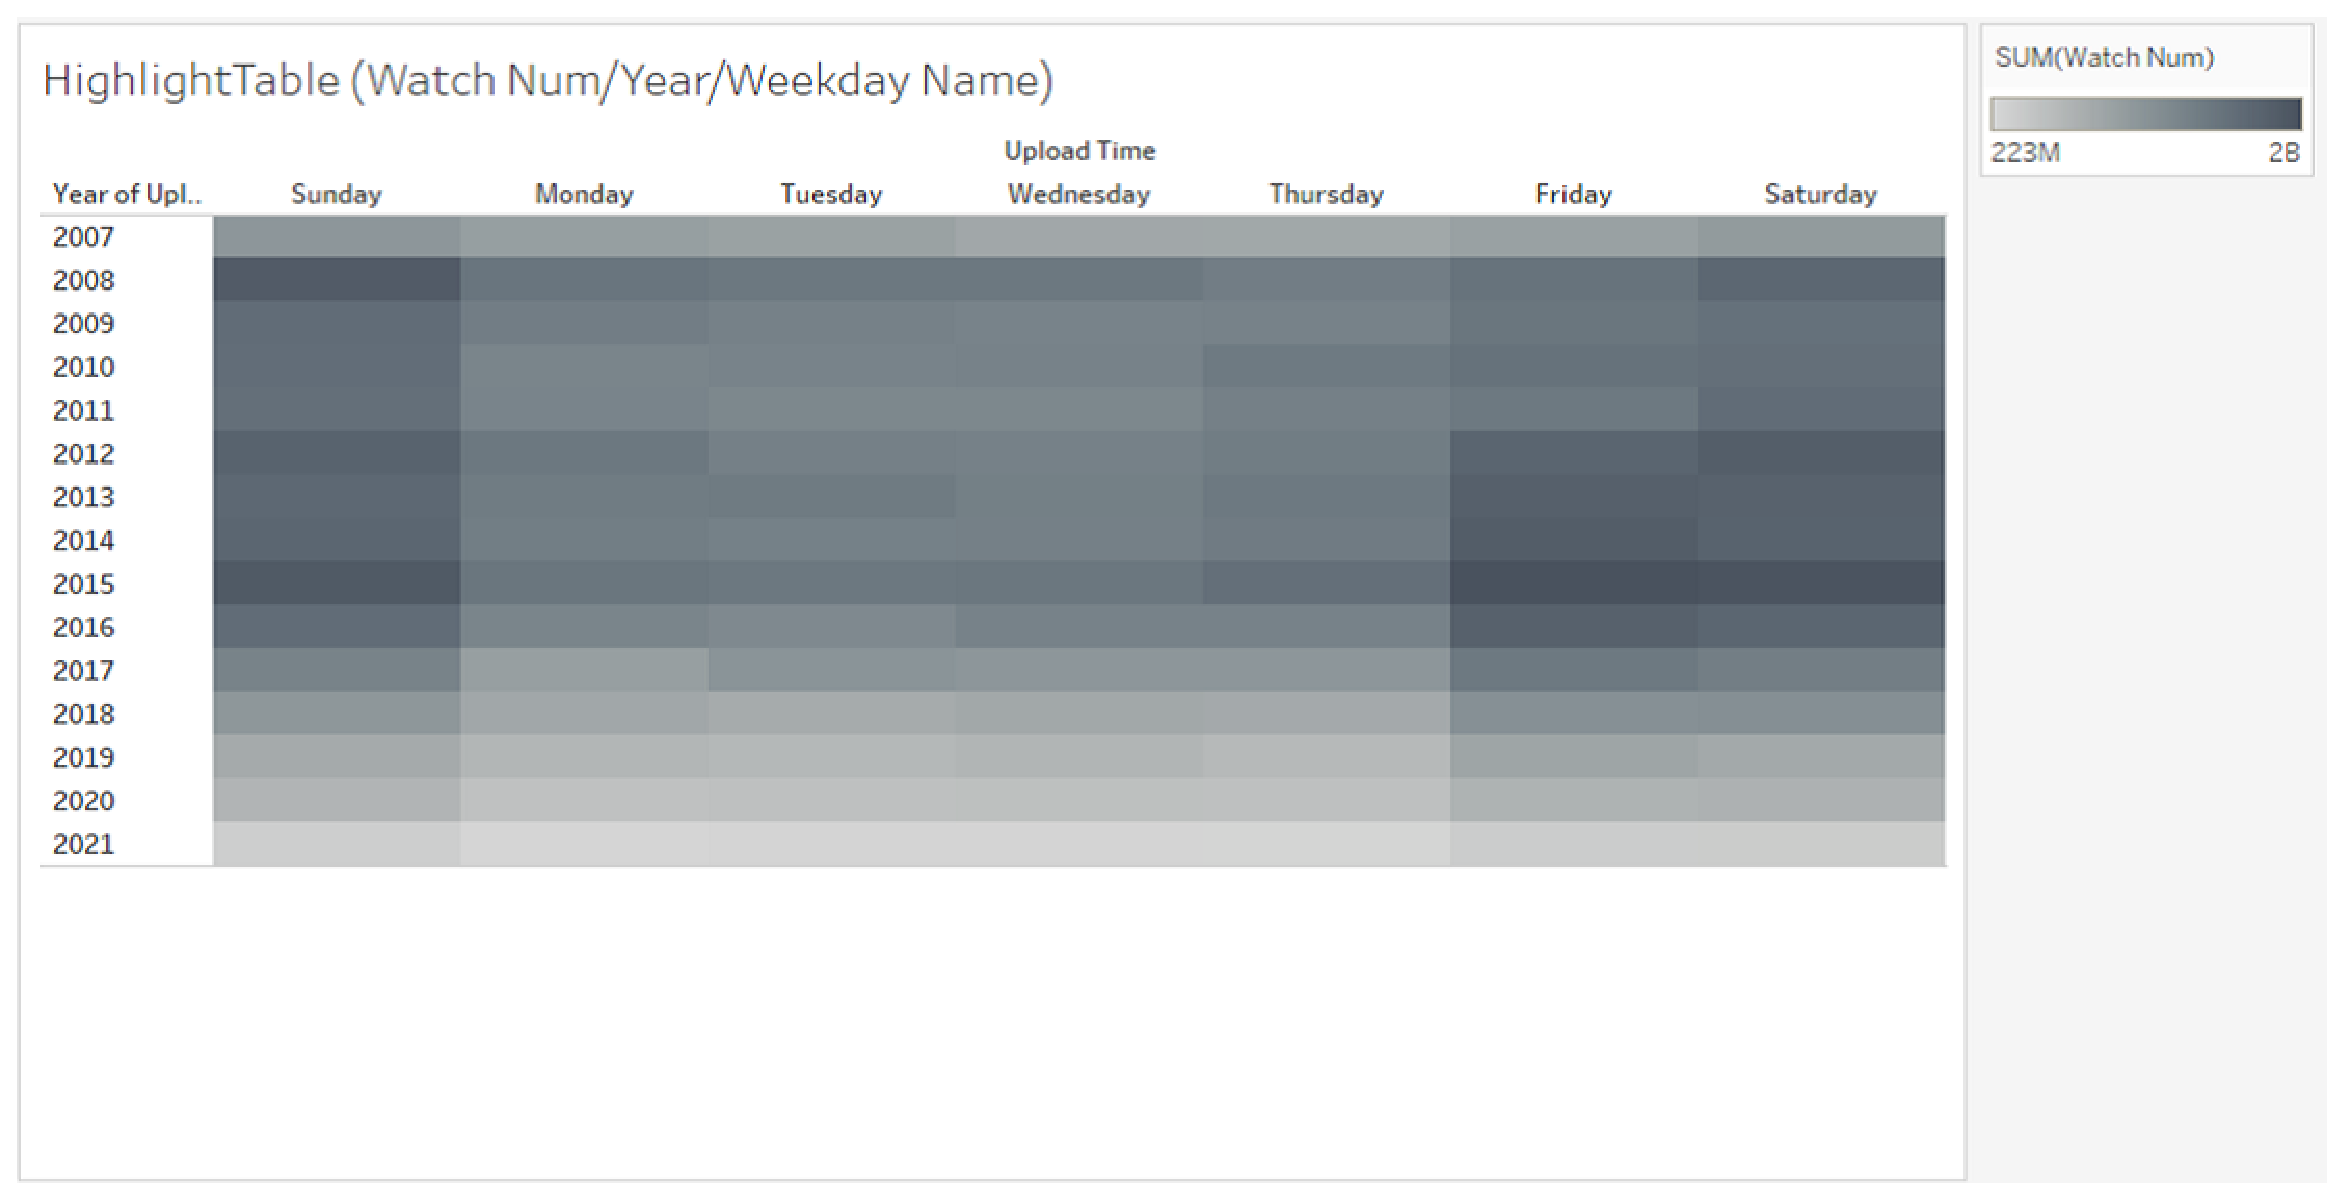
\includegraphics[width=\columnwidth]{./eps/HighlightTable_WatchNum_YearWeekdayName.eps}
    \subcaption{Year/WeekdayName}\label{fig:highlighttable_watchnum_year_weekday}
  \end{minipage}
\vspace{-1.0zh}
  \caption{WatchNum(1)}
  \label{fig:highlighttable_watchnum_year}
\end{figure}
%
\vspace{-2.5zh}
%
\begin{figure}[h]
\vspace{-1.0zh}
  \begin{minipage}[b]{0.49\columnwidth}
    \centering
    \hspace{-1.0zh}
    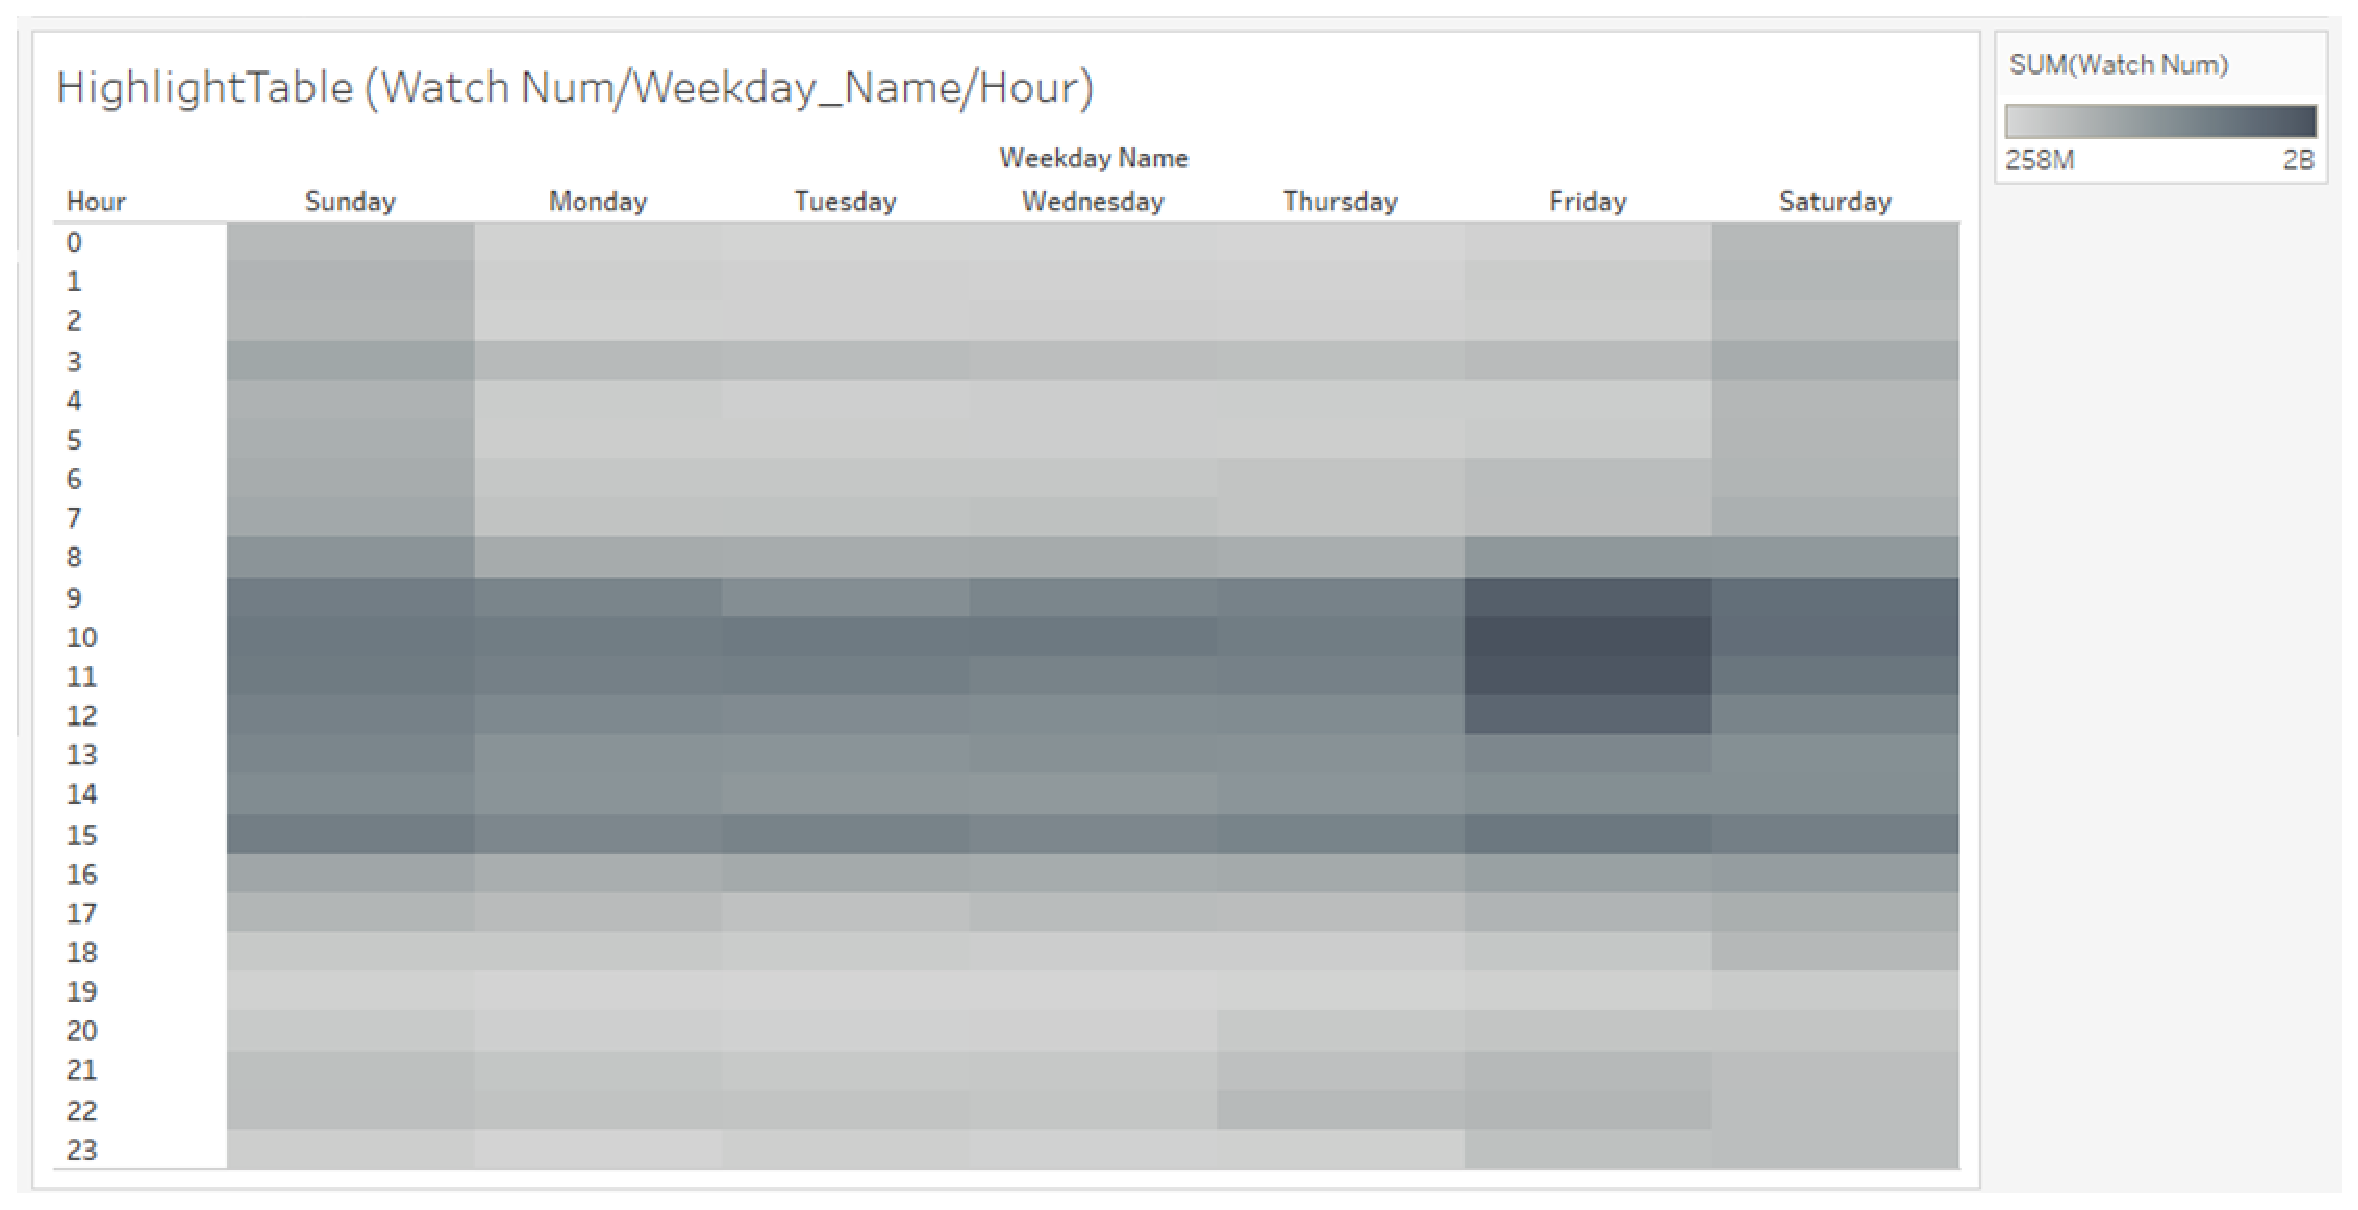
\includegraphics[width=\columnwidth]{./eps/HighlightTable_WatchNum_WeekdayNameHour.eps}
    \subcaption{WeekdayName/Hour}\label{fig:highlighttable_watchnum_weekday_hour}
  \end{minipage}
  %
  \begin{minipage}[b]{0.49\columnwidth}
    \centering
    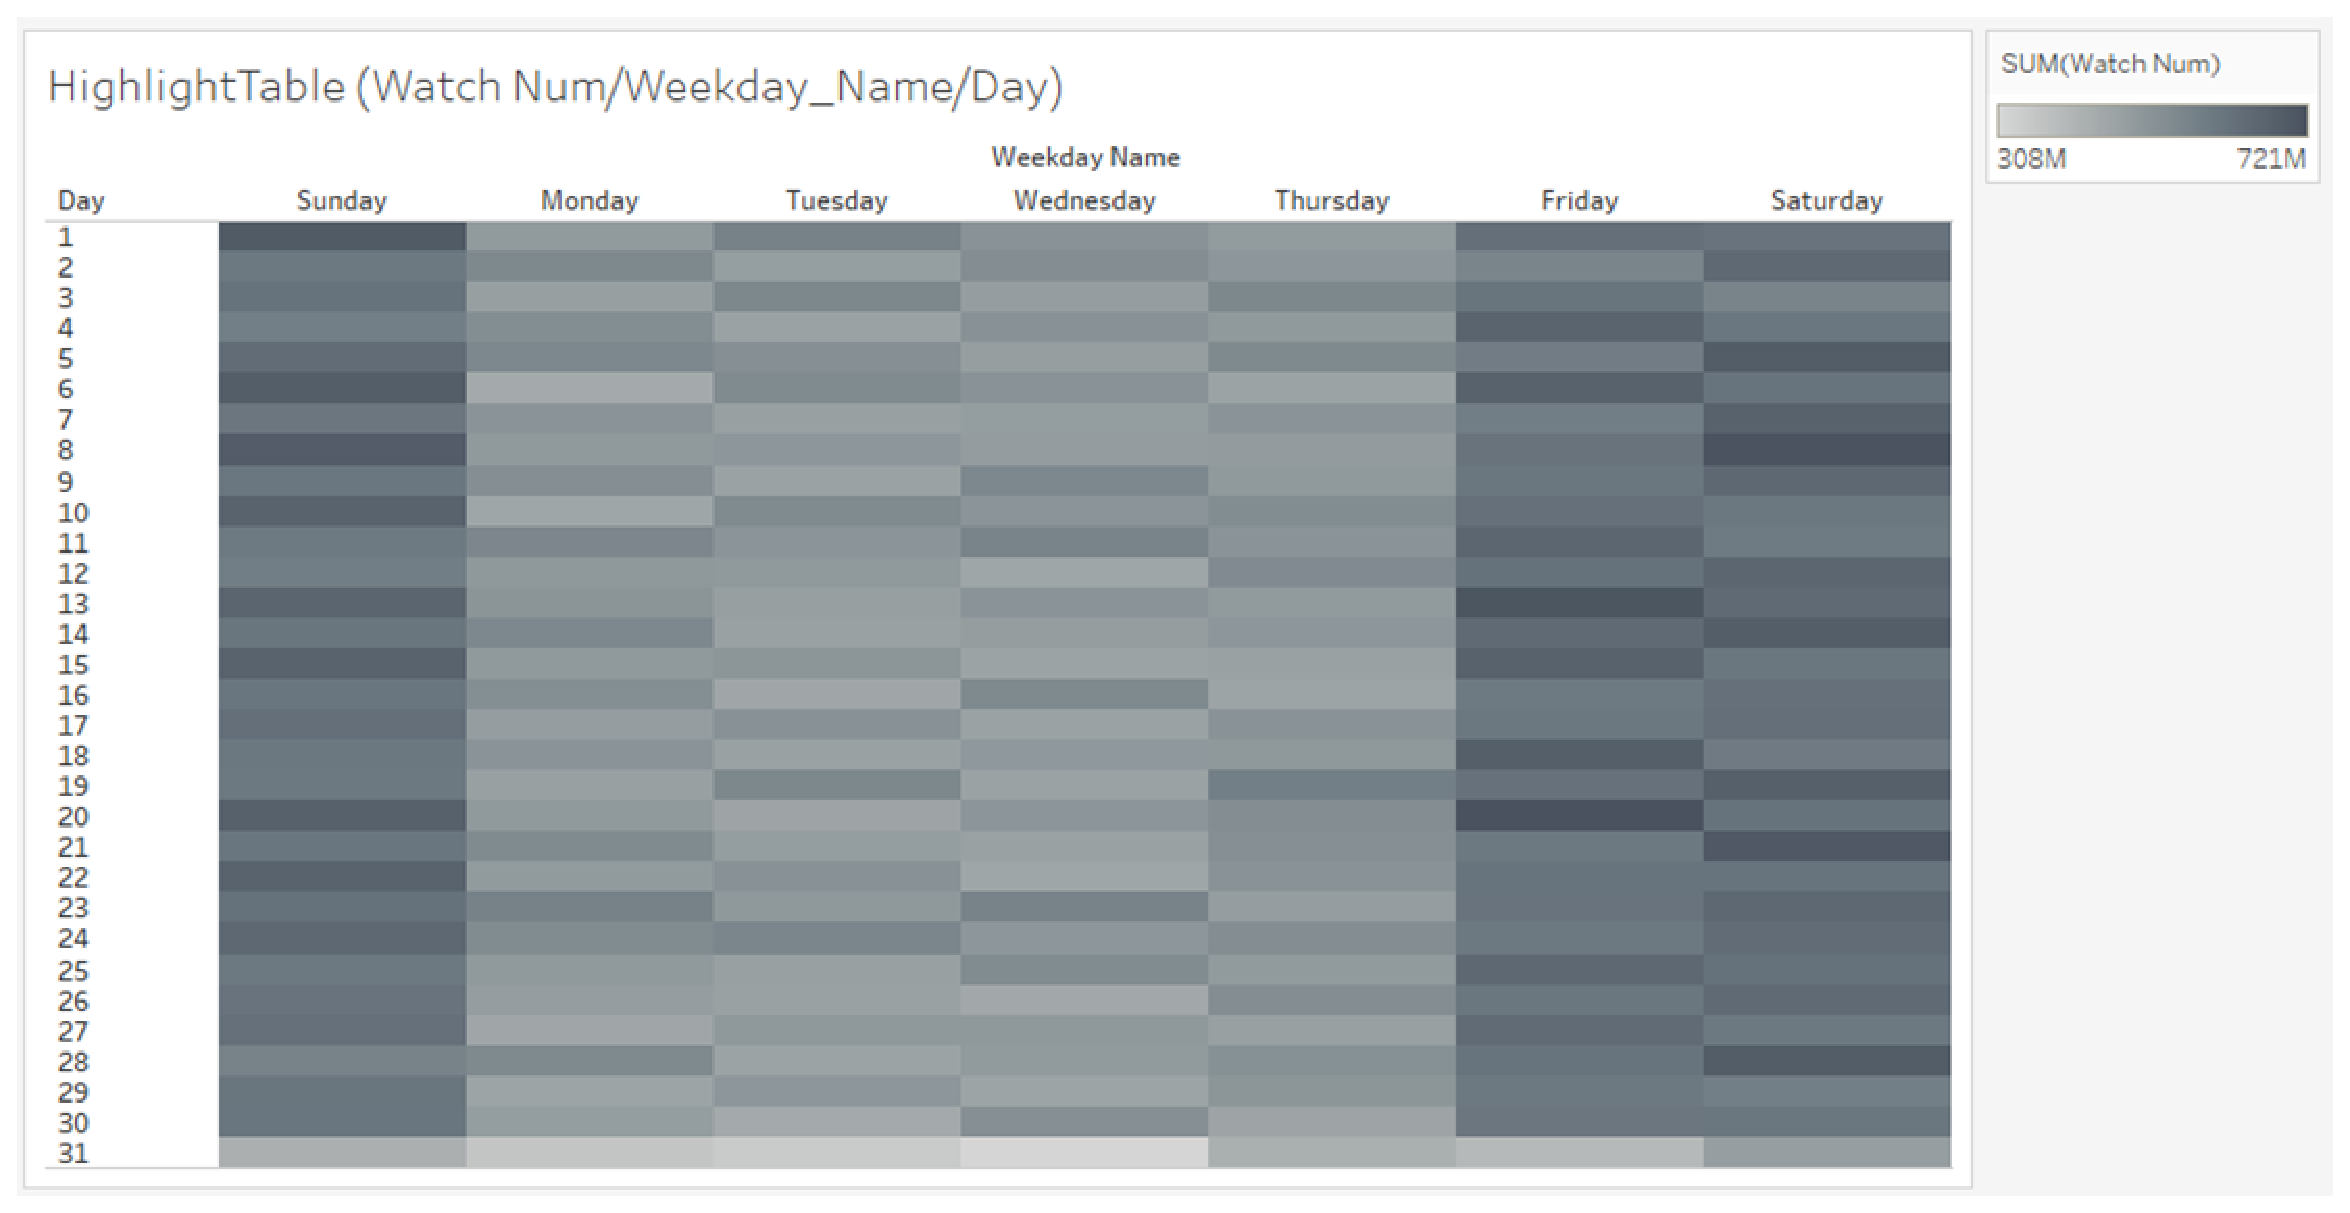
\includegraphics[width=\columnwidth]{./eps/HighlightTable_WatchNum_WeekdayNameDay.eps}
    \subcaption{WeekdayName/Day}\label{fig:highlighttable_watchnum_weekday_day}
  \end{minipage}
  %
  \begin{minipage}[b]{0.49\columnwidth}
    \centering
    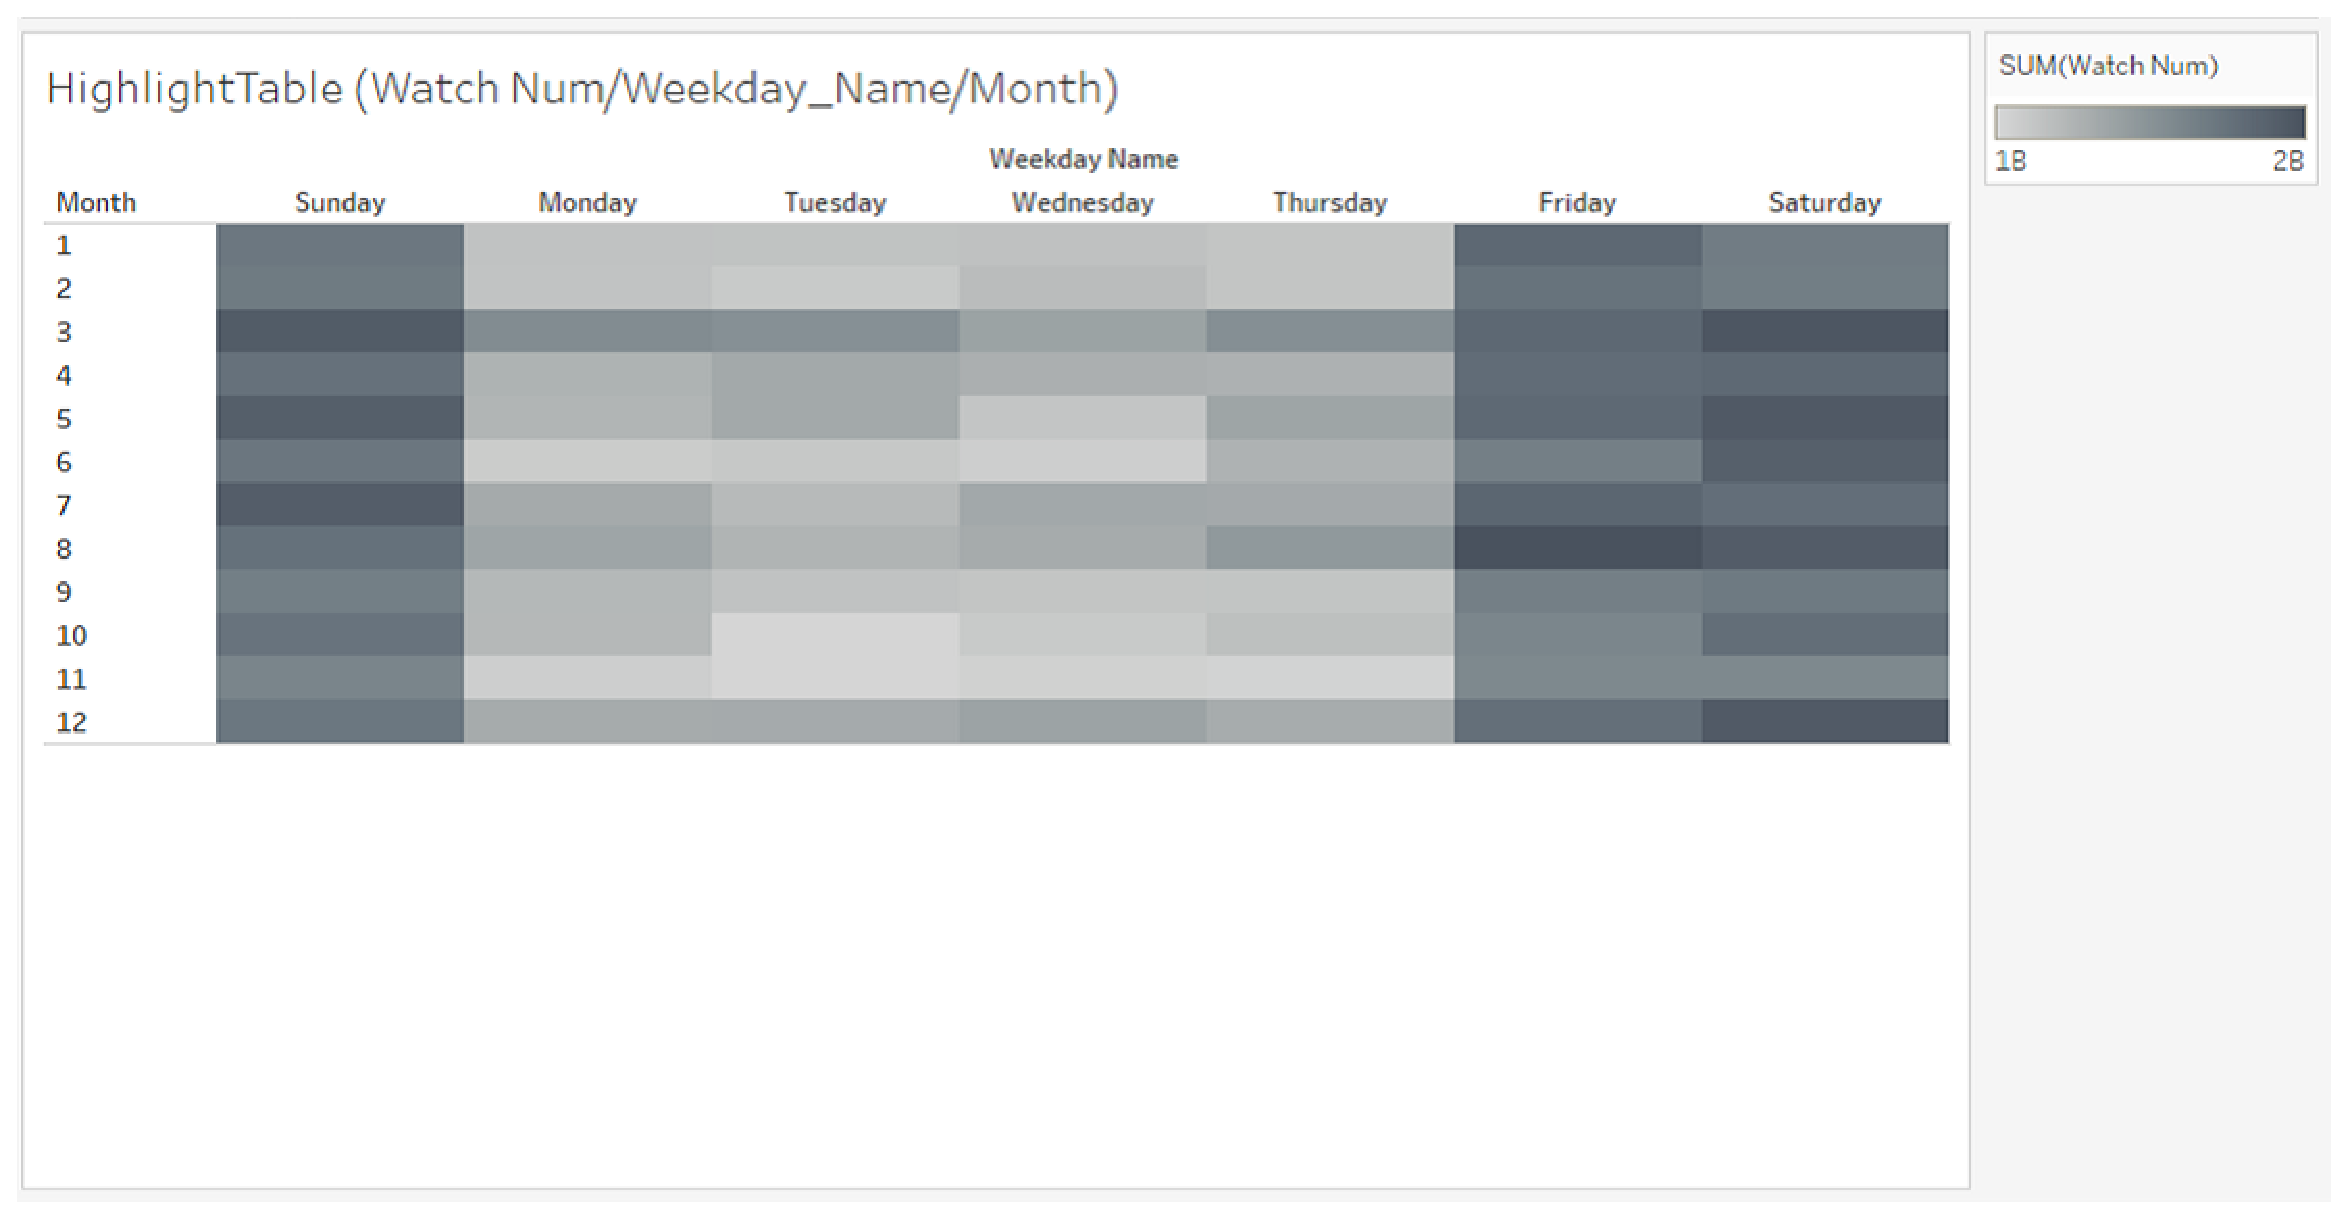
\includegraphics[width=\columnwidth]{./eps/HighlightTable_WatchNum_WeekdayNameMonth.eps}
    \subcaption{WeekdayName/Month}\label{fig:highlighttable_watchnum_weekday_month}
  \end{minipage}
  %
  \begin{minipage}[b]{0.49\columnwidth}
    \centering
    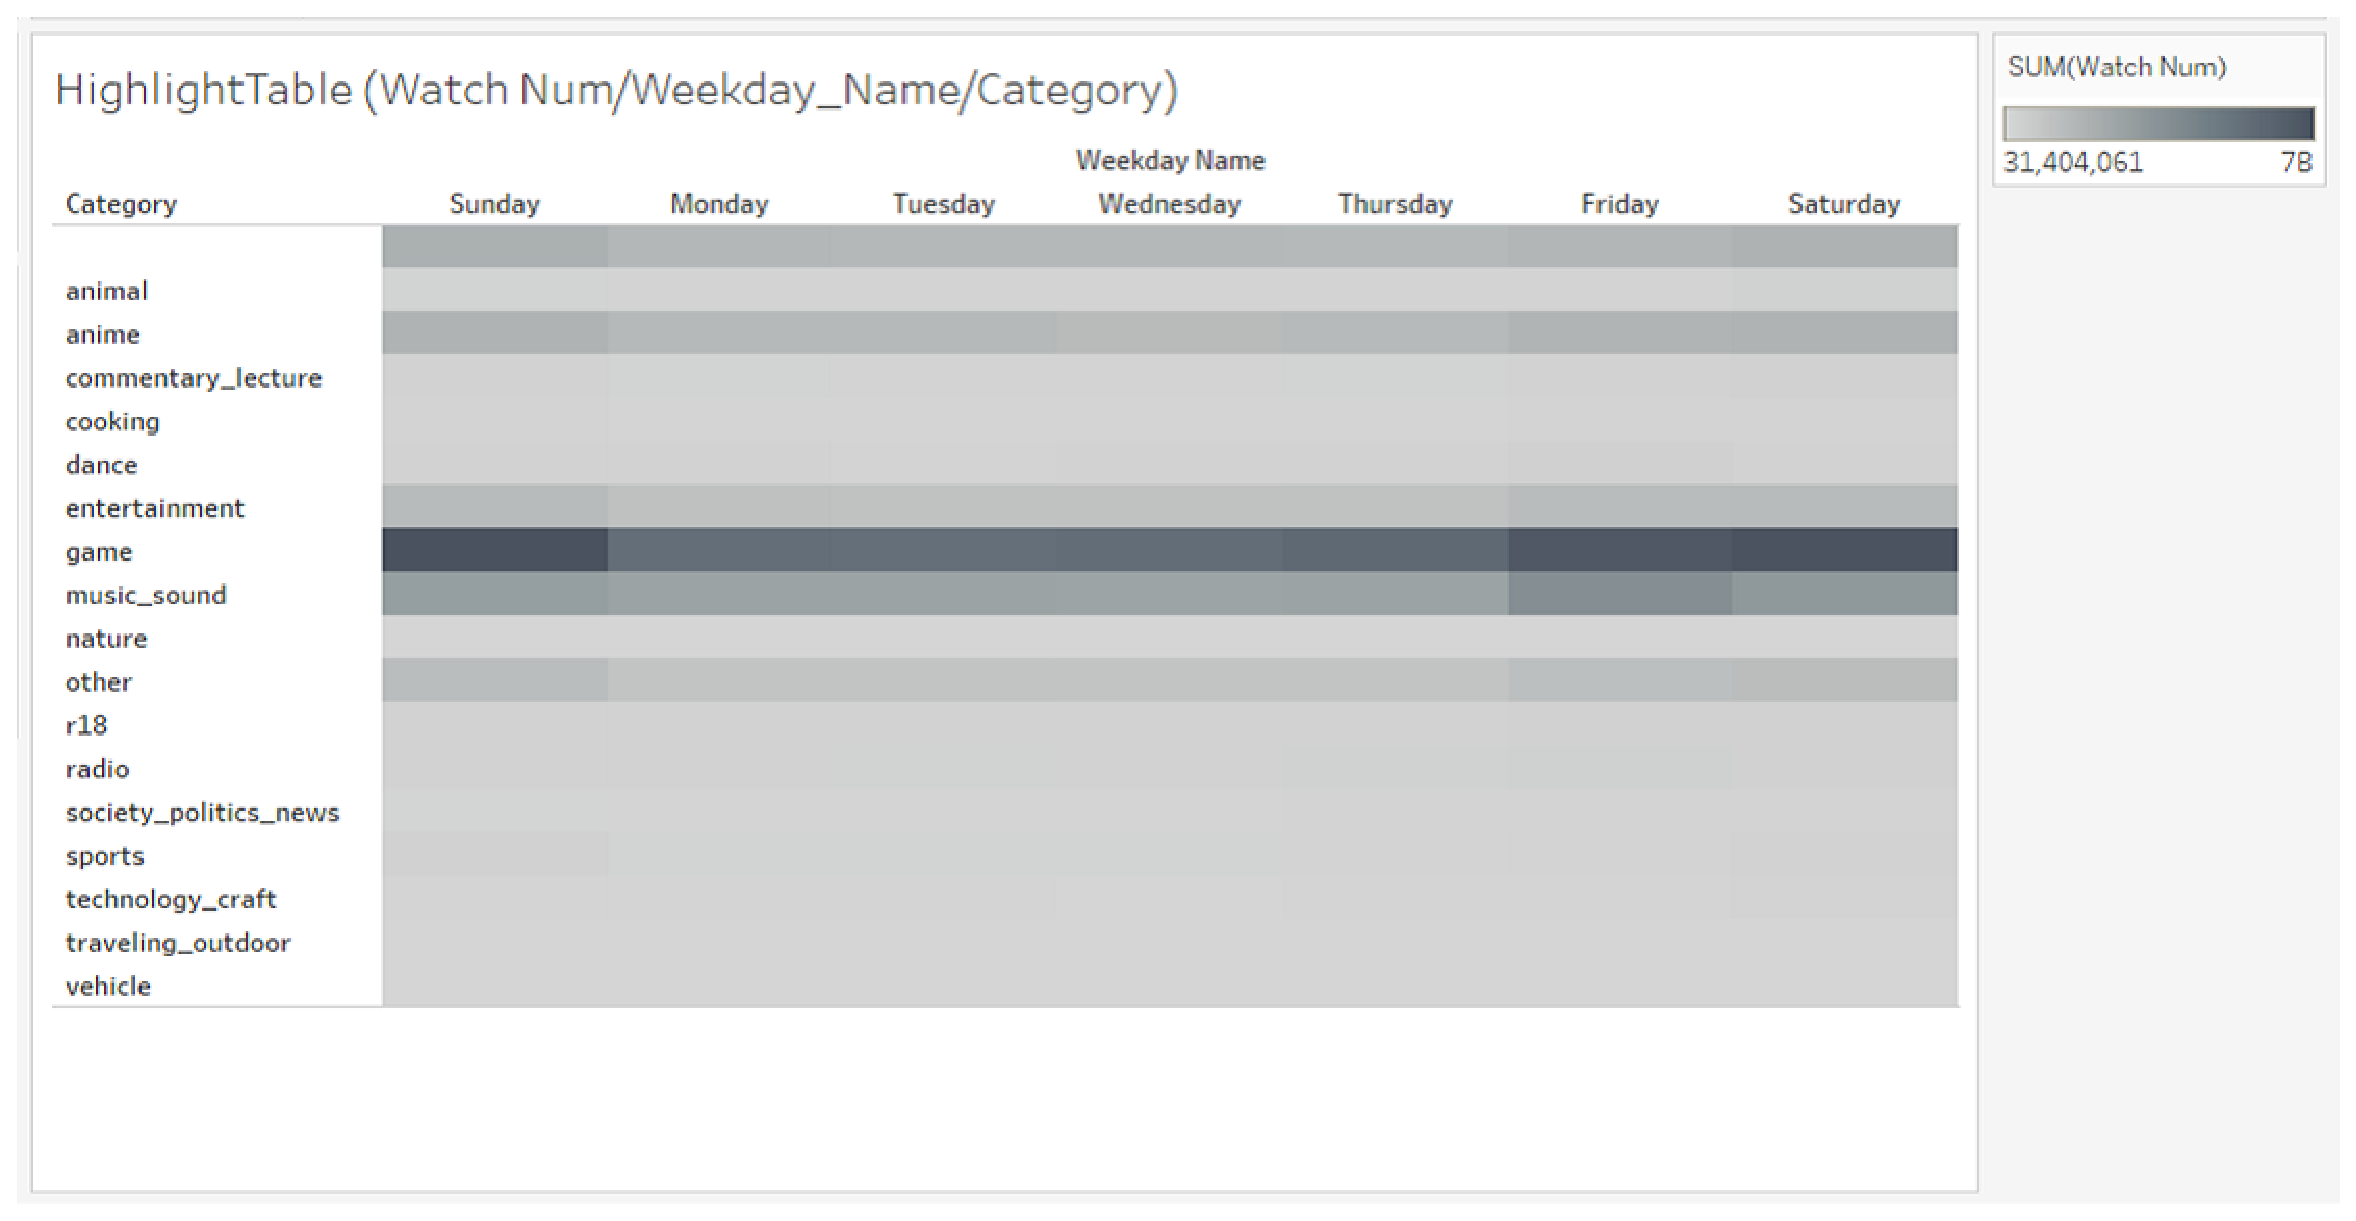
\includegraphics[width=\columnwidth]{./eps/HighlightTable_WatchNum_WeekdayNameCategory.eps}
    \subcaption{WeekdayName/Category}\label{fig:highlighttable_watchnum_weekday_category}
  \end{minipage}
\vspace{-1.0zh}
  \caption{WatchNum(2)}
  \label{fig:highlighttable_watchnum_weekdayname}
%\vspace{-1.0zh}
\end{figure}
\vspace{-1.5zh}

図\ref{fig:highlighttable_watchnum_year_hour}から
図\ref{fig:highlighttable_watchnum_year_weekday}の結果について考察する.
%
年と時間の集計した図\ref{fig:highlighttable_watchnum_year_hour}では,
2014年から2018年までの期間の9時から11時に投稿された動画の閲覧数が多くなる傾向にあった.
%
年と日で集計した図\ref{fig:highlighttable_watchnum_weekday_day}では,
各年単位で集計では,月末や月初など時期による違いは見受けられない.
%
年と月で集計した図\ref{fig:highlighttable_watchnum_weekday_month}では,
3月や8月に投稿された動画の総数が,閲覧数が多くなる傾向にあった.
%
年と曜日で集計した図\ref{fig:highlighttable_watchnum_weekday_year}では,
金曜日から日曜日の3日間の投稿動画数が多い.
%
閲覧数は,投稿時の話題となり,ピックアップされることによって,閲覧者が増える場合もある.
このため,投稿日時で,閲覧数が増える時期などが,可視化できた.

%-------------------------------------
また,図\ref{fig:highlighttable_watchnum_weekday_hour}から
図\ref{fig:highlighttable_watchnum_weekday_category}の結果について考察する.
%
時間と曜日で集計した図\ref{fig:highlighttable_watchnum_weekday_hour}では,
9時から15時までの閲覧数が多く,が多く,金曜日の9時から12時の間が最も投稿が盛んである.
%
日と曜日で集計した図\ref{fig:highlighttable_watchnum_weekday_day}では,
土曜日の朝8時に動画投稿が集中していた.
%
月と曜日で集計した図\ref{fig:highlighttable_watchnum_weekday_month}では,
12月の土曜日に動画投稿が集中していた.
%
カテゴリと曜日で集計した図\ref{fig:highlighttable_watchnum_weekday_category}では,
金曜日と日曜日に音楽の投稿動画が多い.
%
このことから,曜日特有の投稿状況を可視化することができたと言える.


\newpage
\subsection{HighlightTable分析 - CommentNum}
コメント数を集計値として,可視化した結果を図\ref{fig:highlighttable_comment_num_year}および
図\ref{fig:highlighttable_comment_num_week}に示す.
%
図\ref{fig:highlighttable_comment_num_year}は縦軸が年であり,
横軸は時間,日,月,曜日の単位で集計している.
図\ref{fig:highlighttable_comment_num_week}は横軸が曜日であり,
縦軸は時間,日,月,カテゴリで集計している.

\vspace{-1.5zh}
\begin{figure}[h]
  \begin{minipage}[b]{0.49\columnwidth}
    \centering
    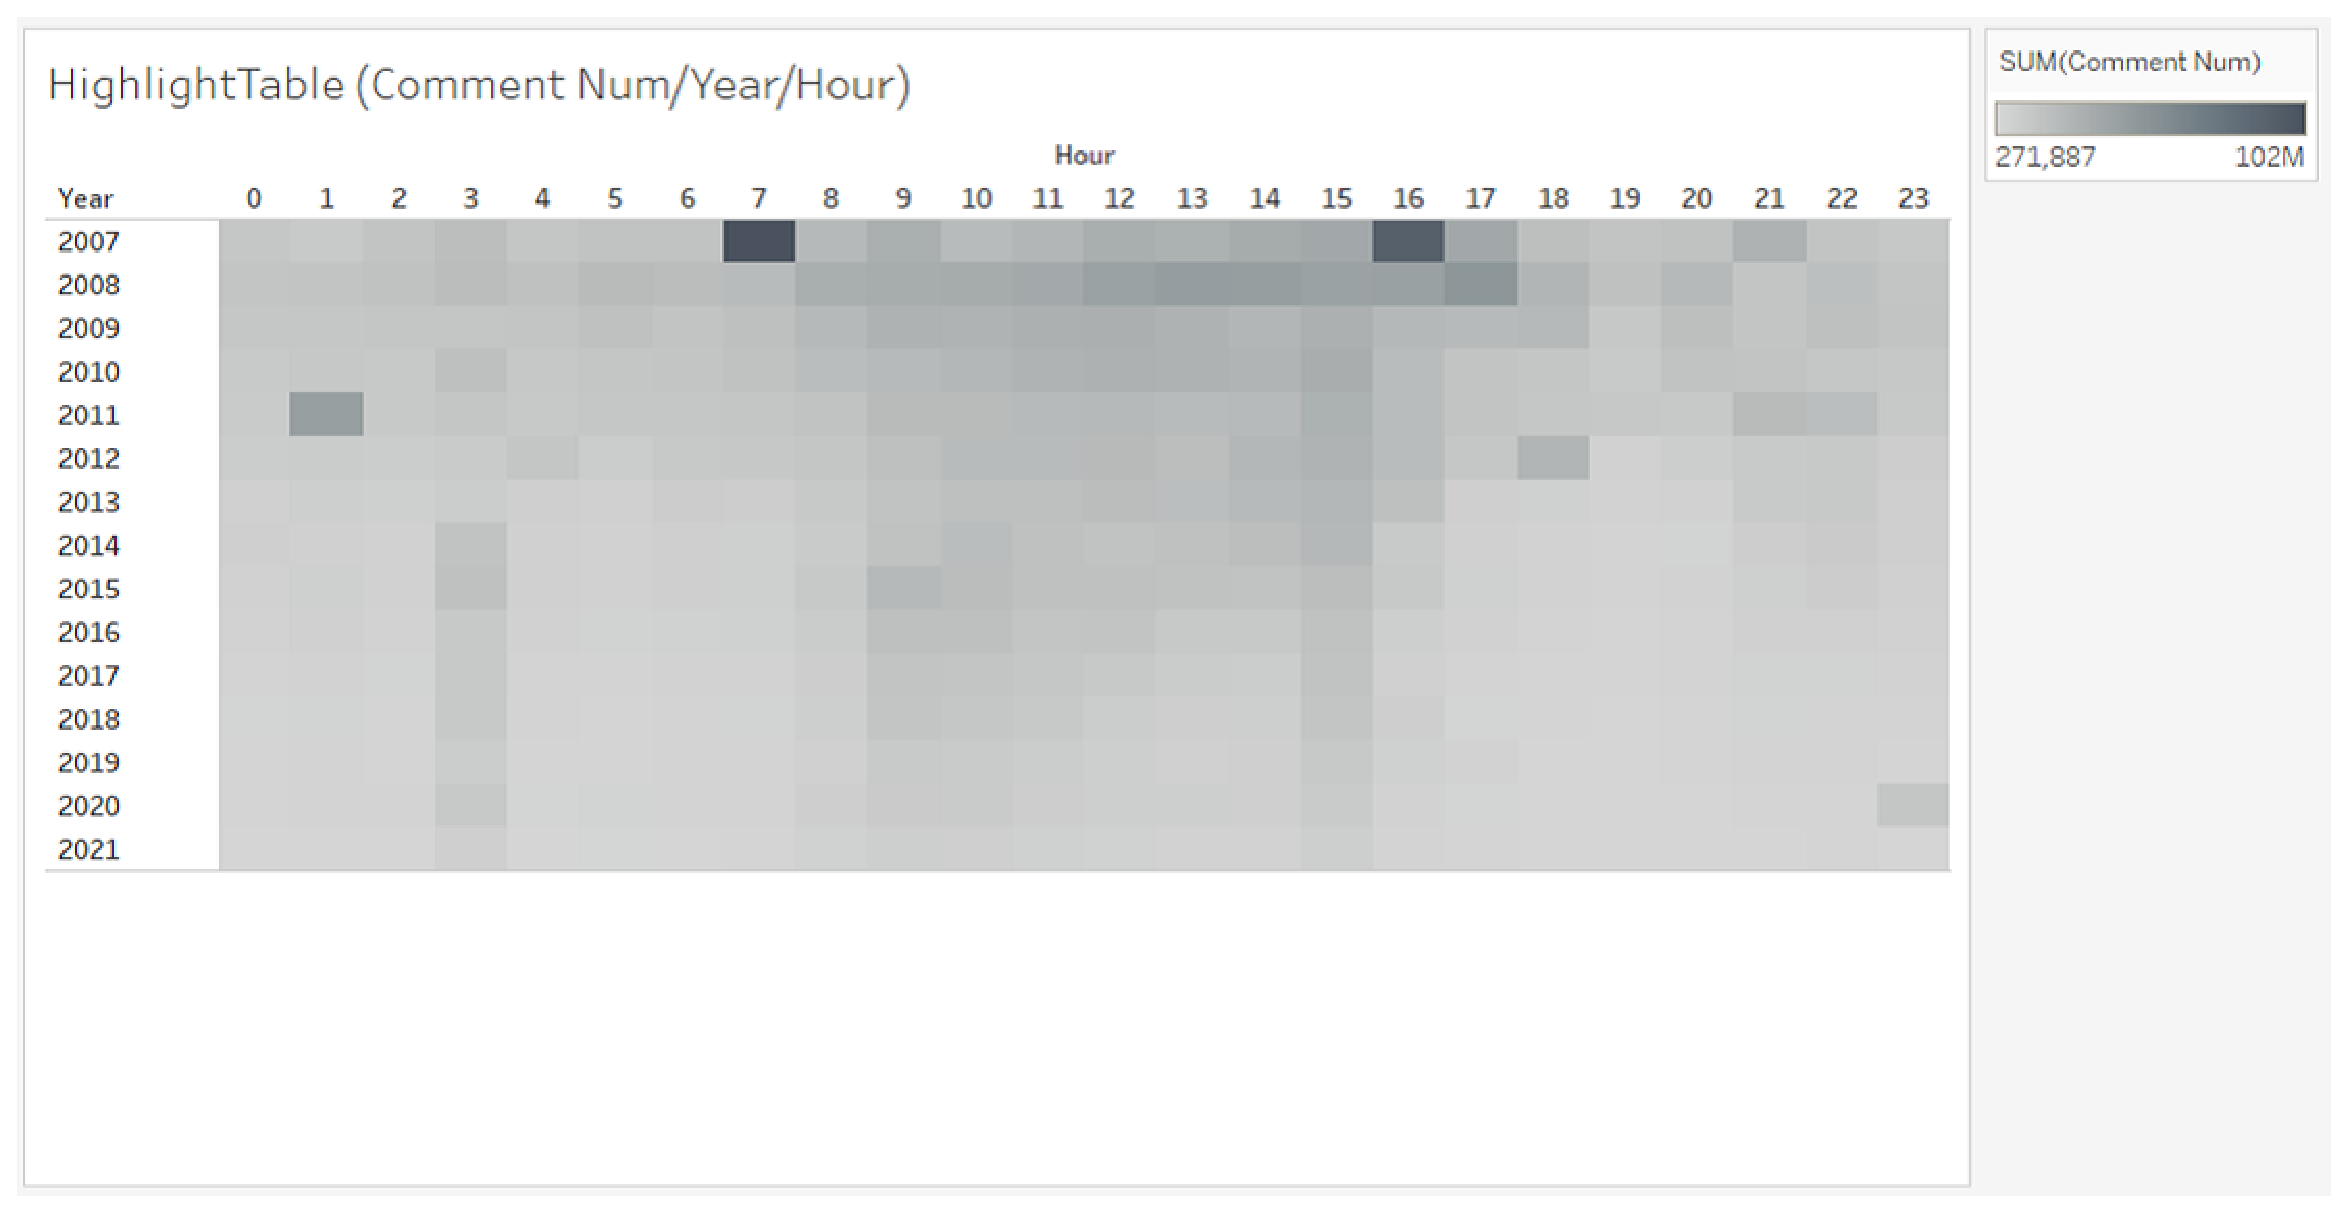
\includegraphics[width=\columnwidth]{./eps/HighlightTable_CommentNum_YearHour.eps}
    \subcaption{Year/Hour}
    \label{fig:highlighttable_comment_num_yearhour}
  \end{minipage}
  %
  \begin{minipage}[b]{0.49\columnwidth}
    \centering
    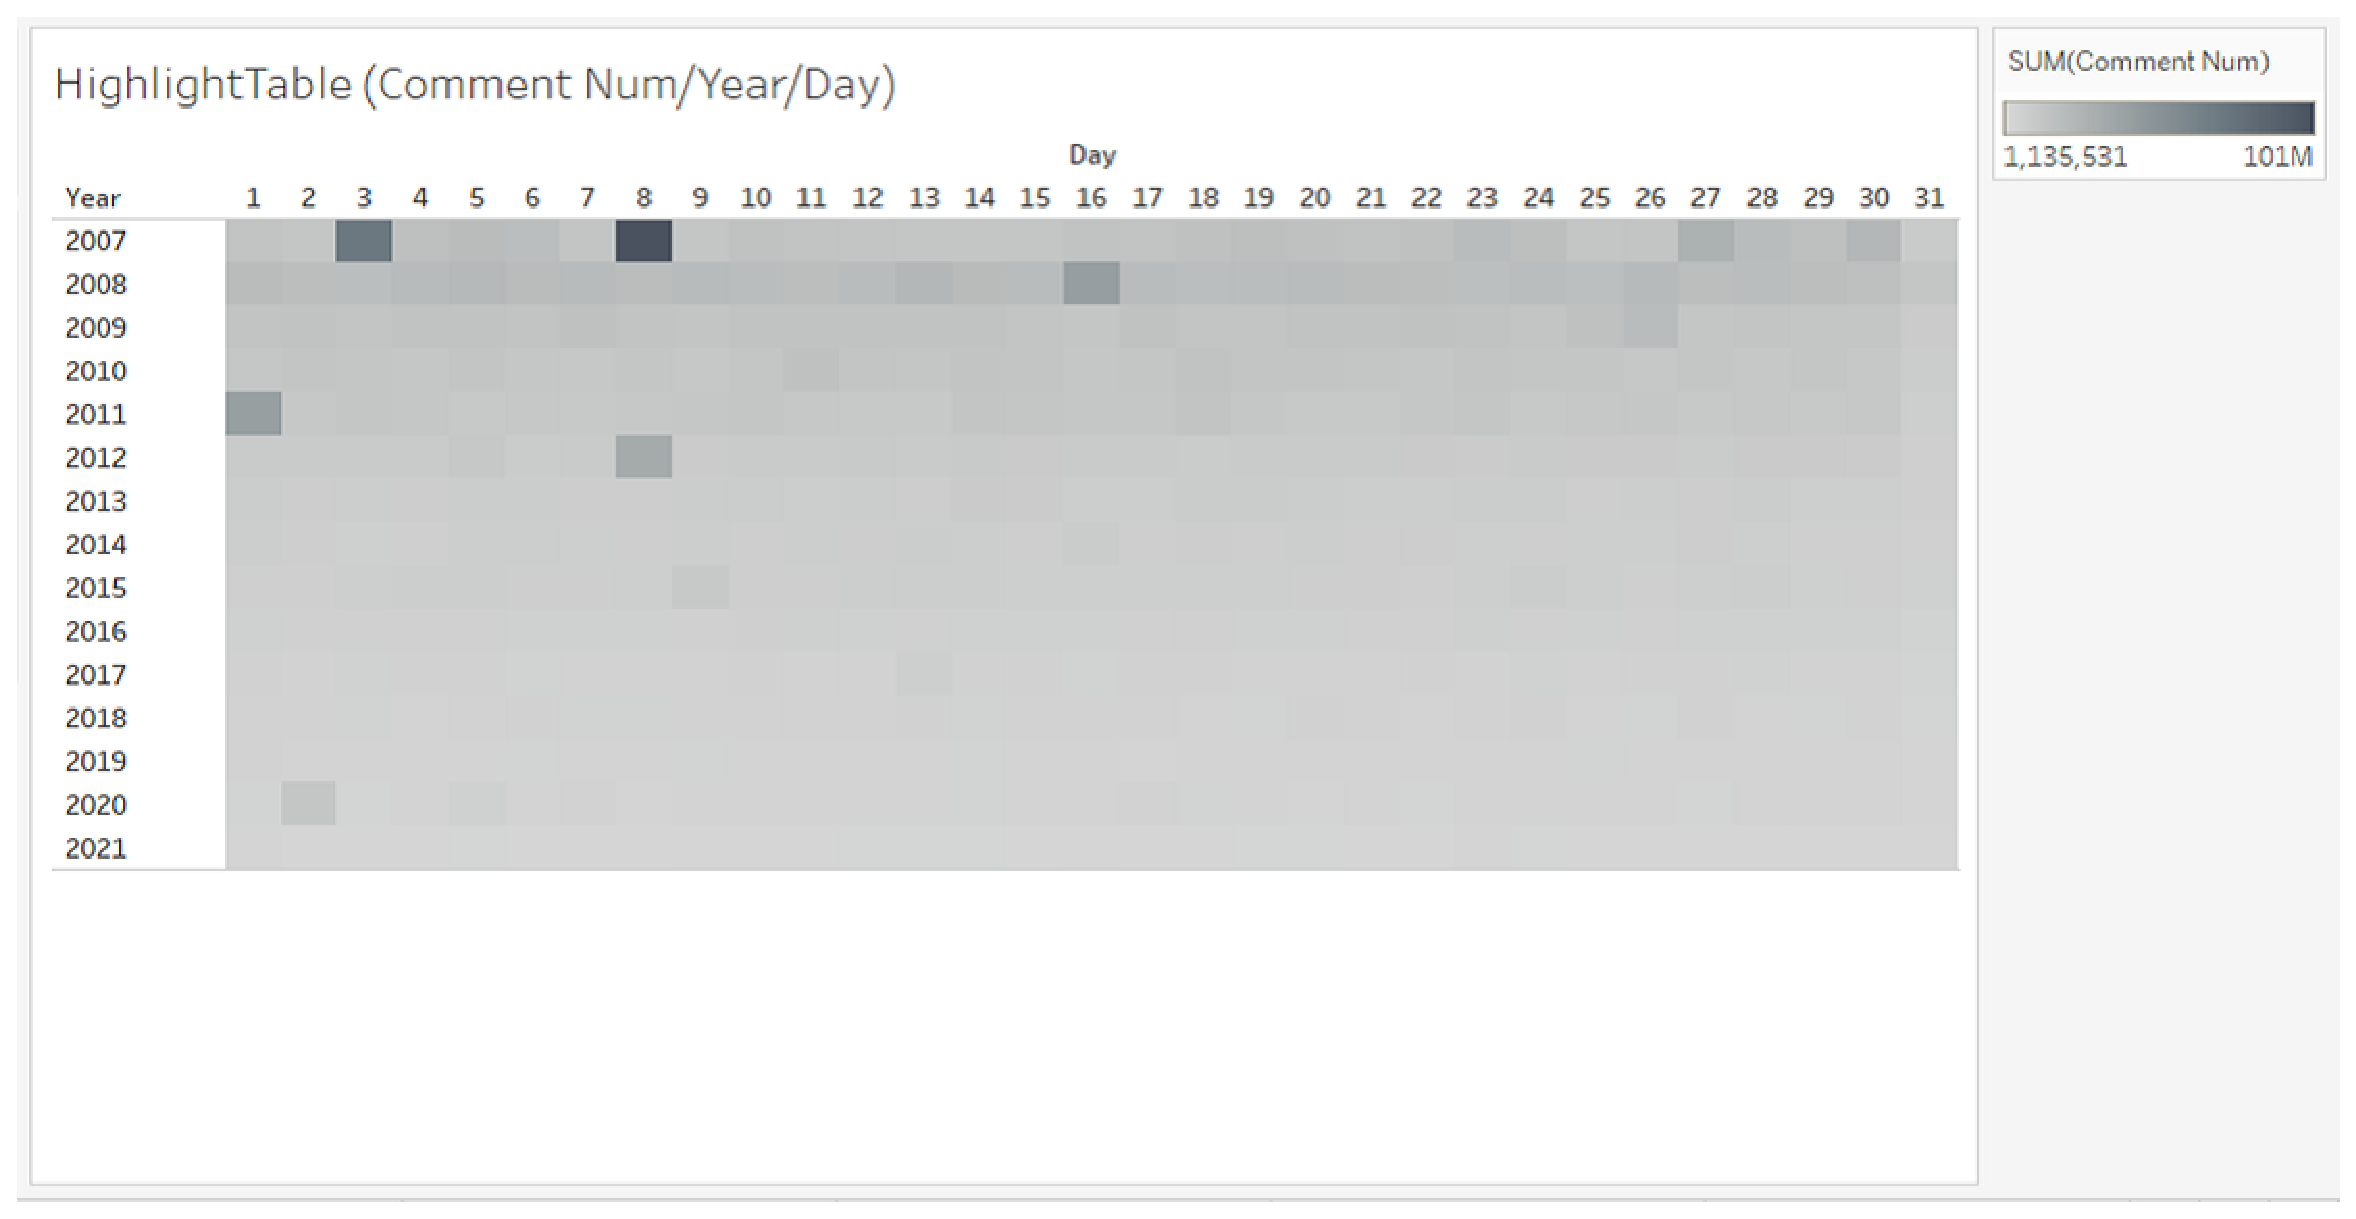
\includegraphics[width=\columnwidth]{./eps/HighlightTable_CommentNum_YearDay.eps}
    \subcaption{Year/Day}
    \label{fig:highlighttable_comment_num_yearday}
  \end{minipage}
  %
  \begin{minipage}[b]{0.49\columnwidth}
    \centering
    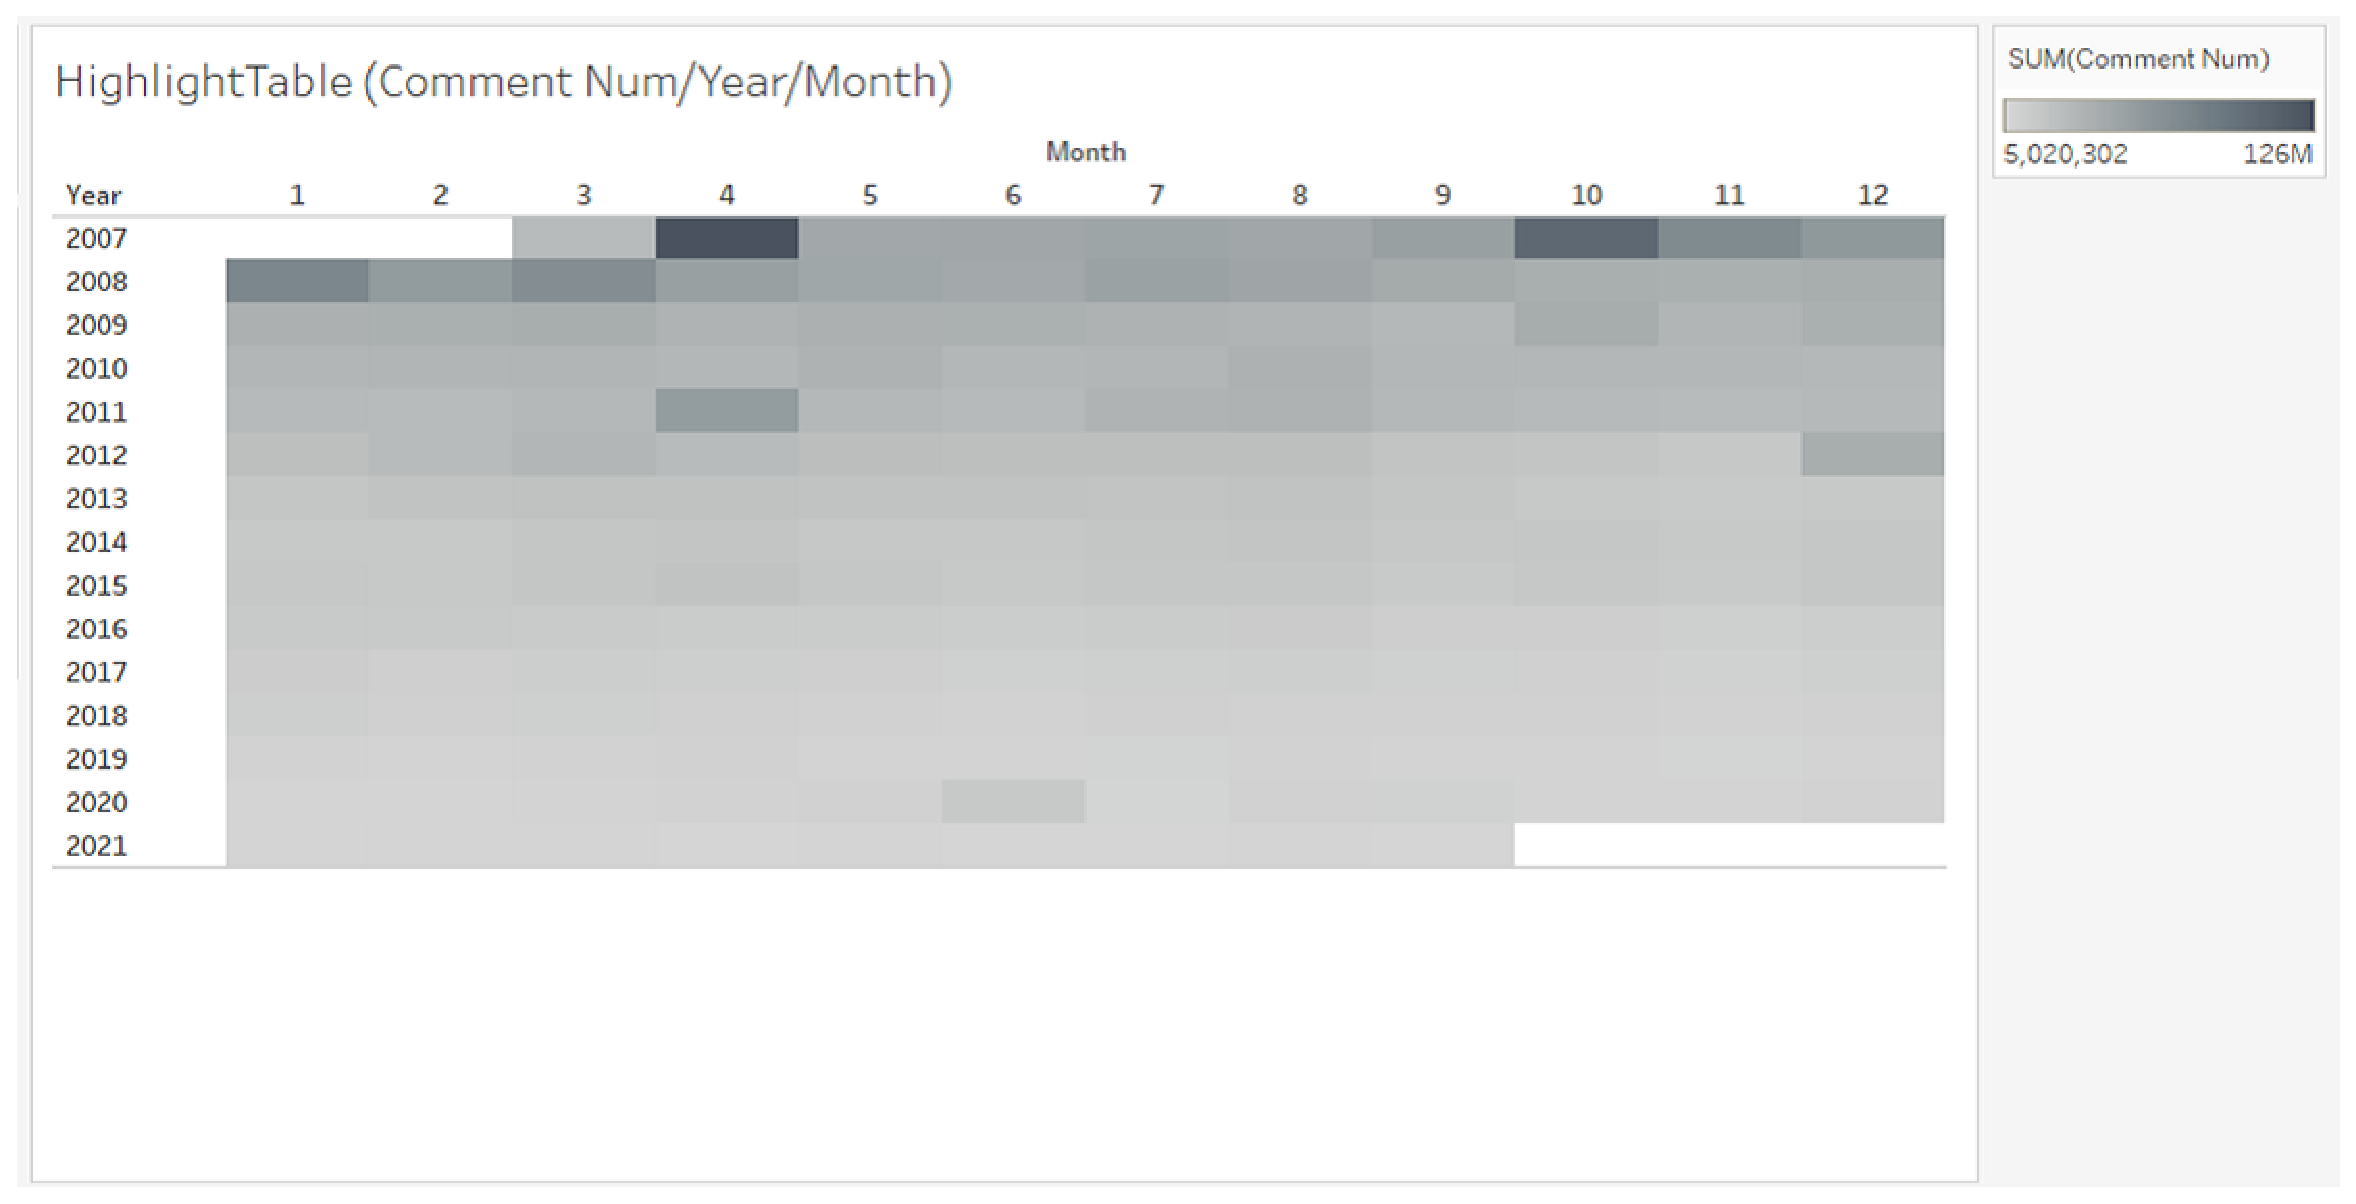
\includegraphics[width=\columnwidth]{./eps/HighlightTable_CommentNum_YearMonth.eps}
    \subcaption{Year/Month}
    \label{fig:highlighttable_comment_num_yearmonth}
  \end{minipage}
  %
  \begin{minipage}[b]{0.49\columnwidth}
    \centering
    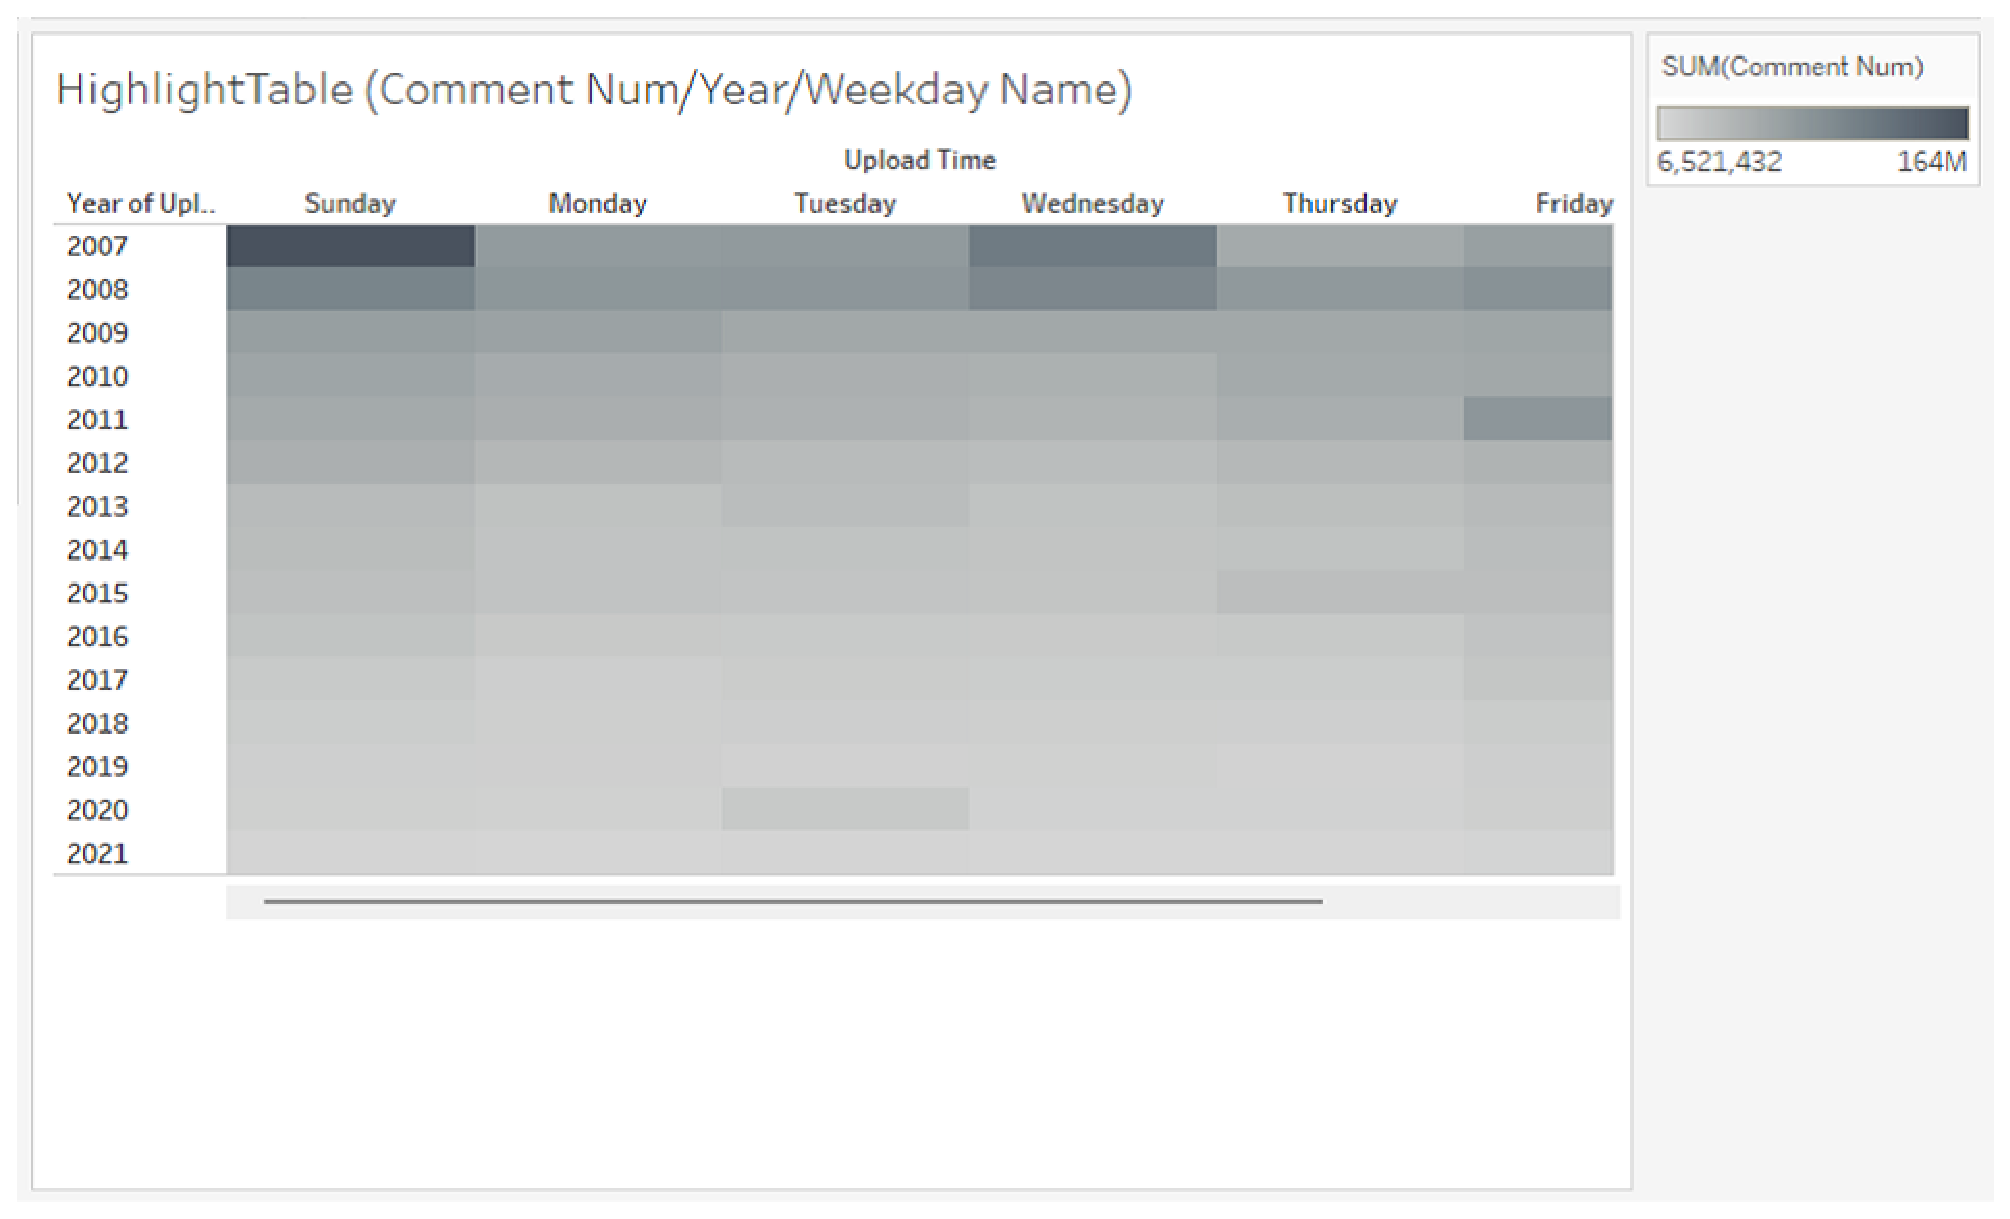
\includegraphics[width=\columnwidth]{./eps/HighlightTable_CommentNum_YearWeekdayName.eps}
    \subcaption{YearWeekday/Name}
    \label{fig:highlighttable_comment_num_yearweekdayname}
  \end{minipage}
\vspace{-1.0zh}
  \caption{CommentNum(1)}
  \label{fig:highlighttable_comment_num_year}
\vspace{-1.0zh}
\end{figure}
%
\vspace{-2.5zh}
%
\begin{figure}[h]
  \hspace{-1.0zh}
  \begin{minipage}[b]{0.49\columnwidth}
    \centering
    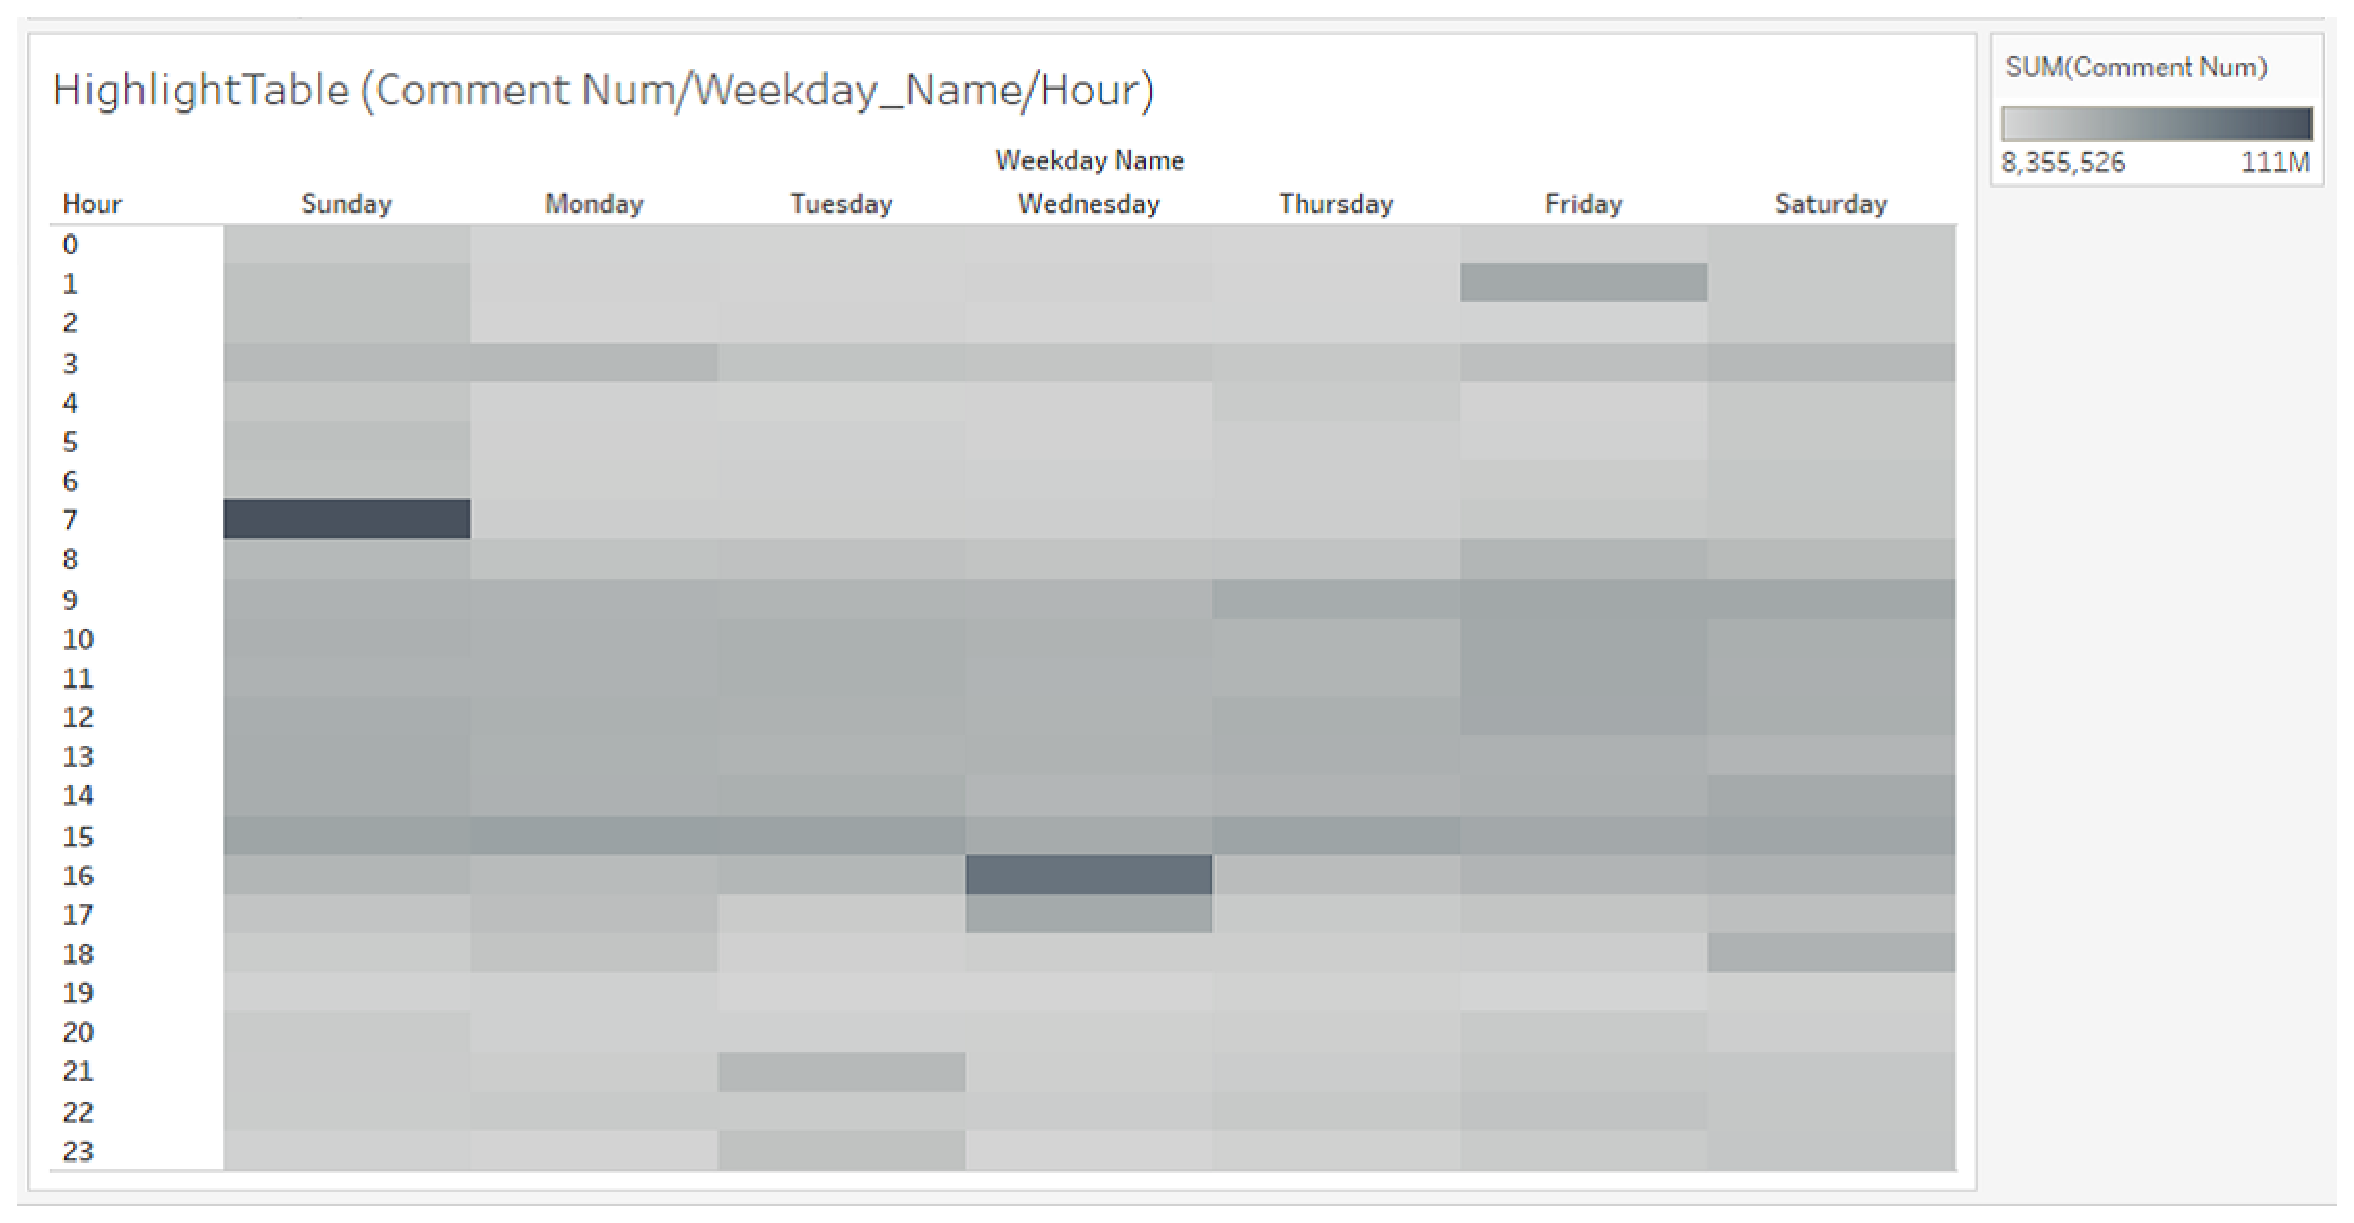
\includegraphics[width=\columnwidth]{./eps/HighlightTable_CommentNum_WeekdayNameHour.eps}
    \subcaption{WeekdayName/Hour}
    \label{fig:highlighttable_comment_num_weekdaynameHour}
  \end{minipage}
  %
  \begin{minipage}[b]{0.49\columnwidth}
    \centering
    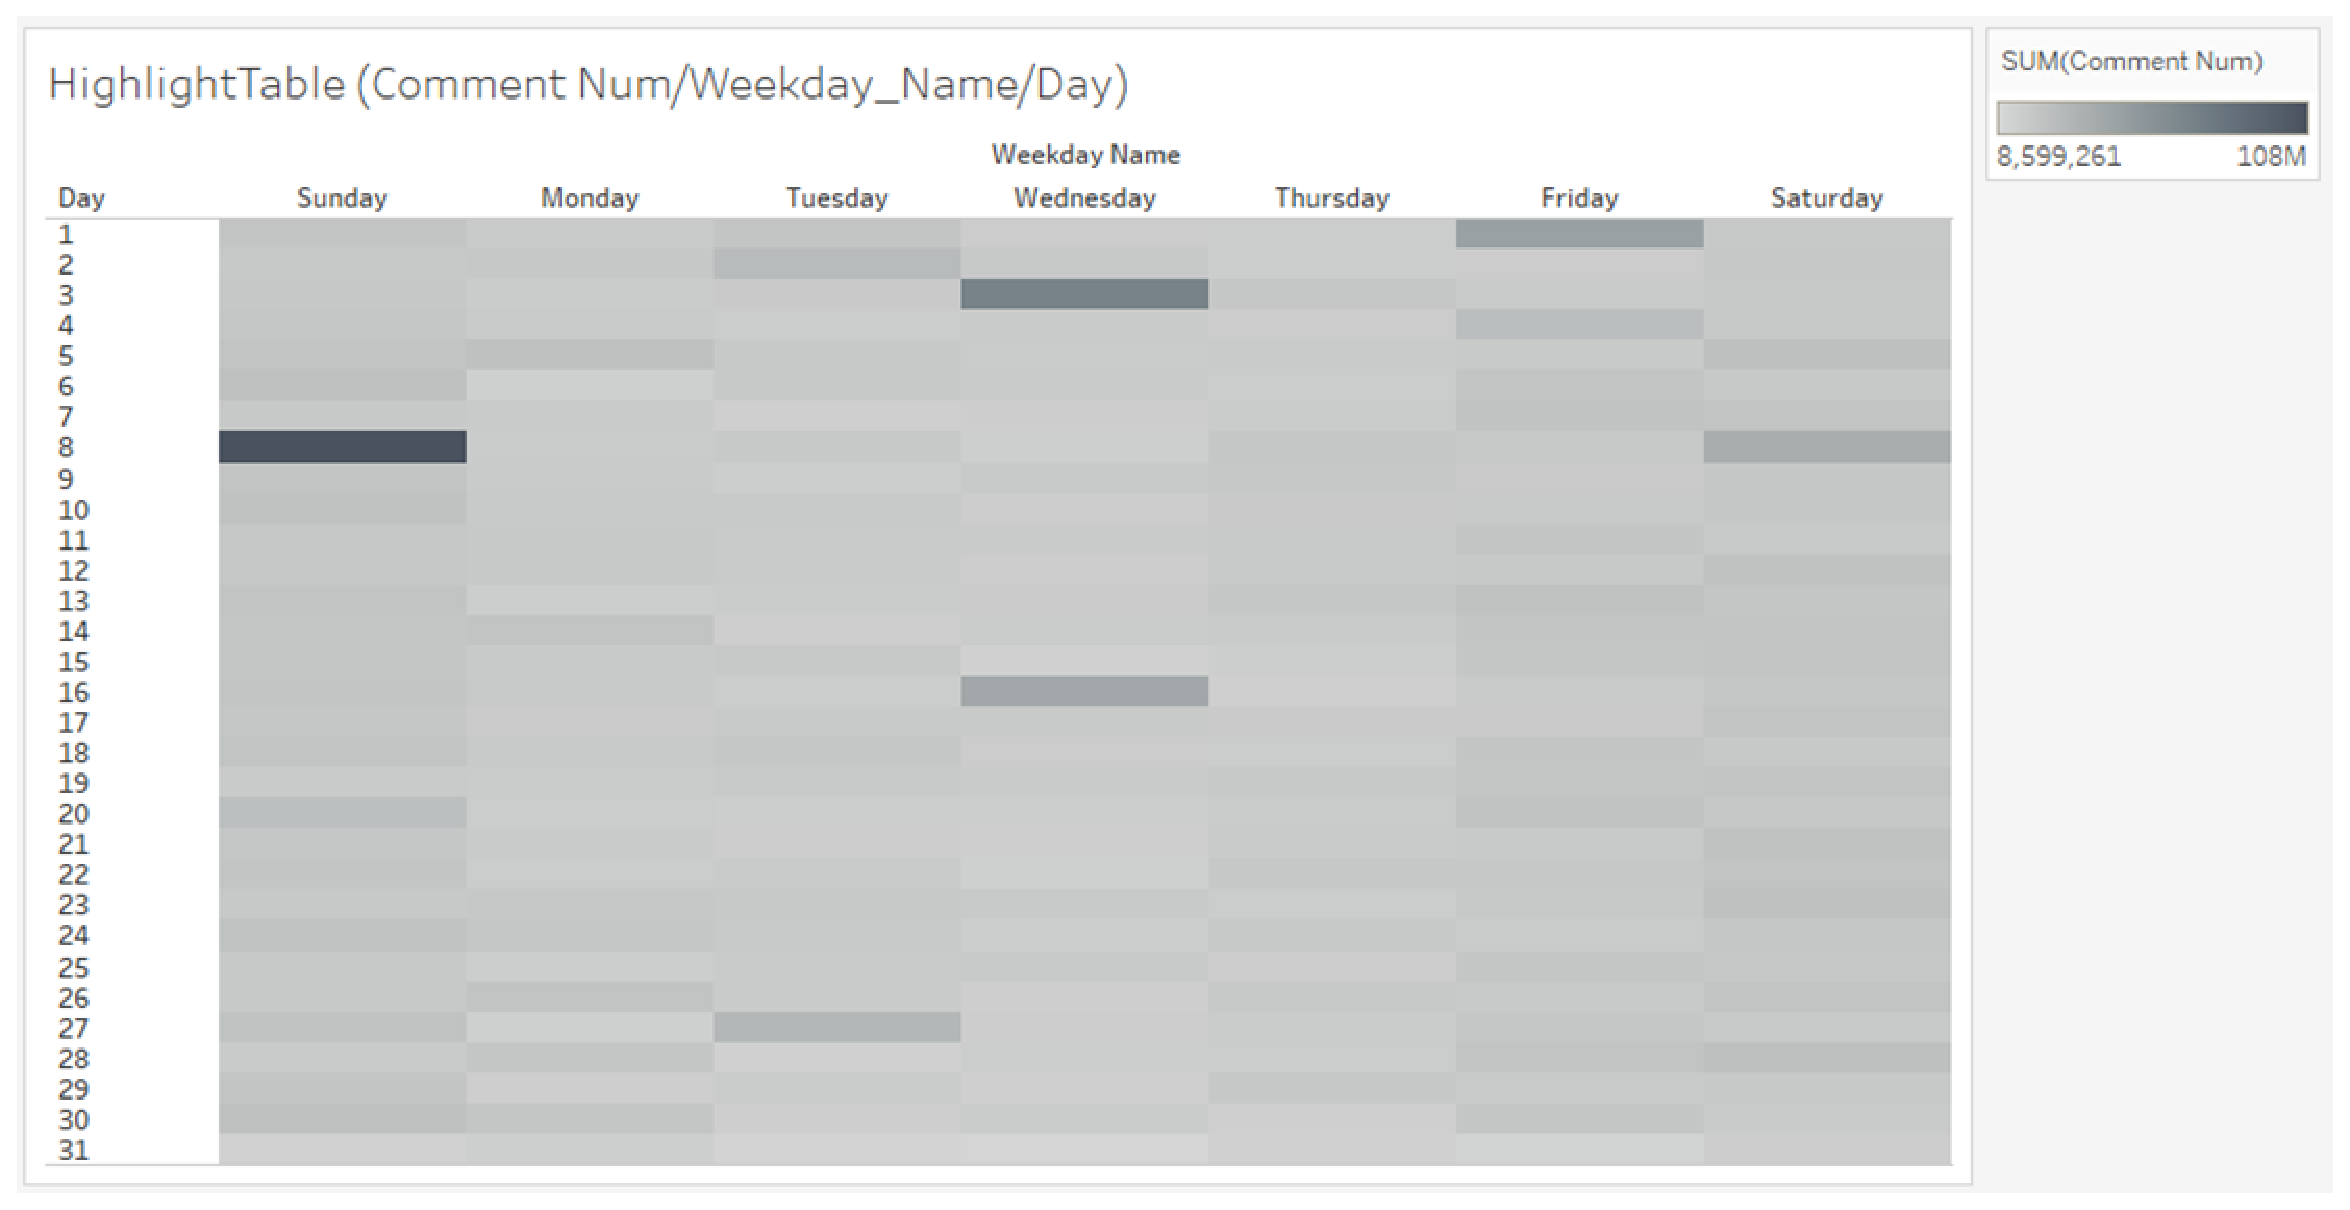
\includegraphics[width=\columnwidth]{./eps/HighlightTable_CommentNum_WeekdayNameDay.eps}
    \subcaption{WeekdayName/Day}
    \label{fig:highlighttable_comment_num_weekdaynameDay}
  \end{minipage}
  %
  \begin{minipage}[b]{0.49\columnwidth}
    \centering
    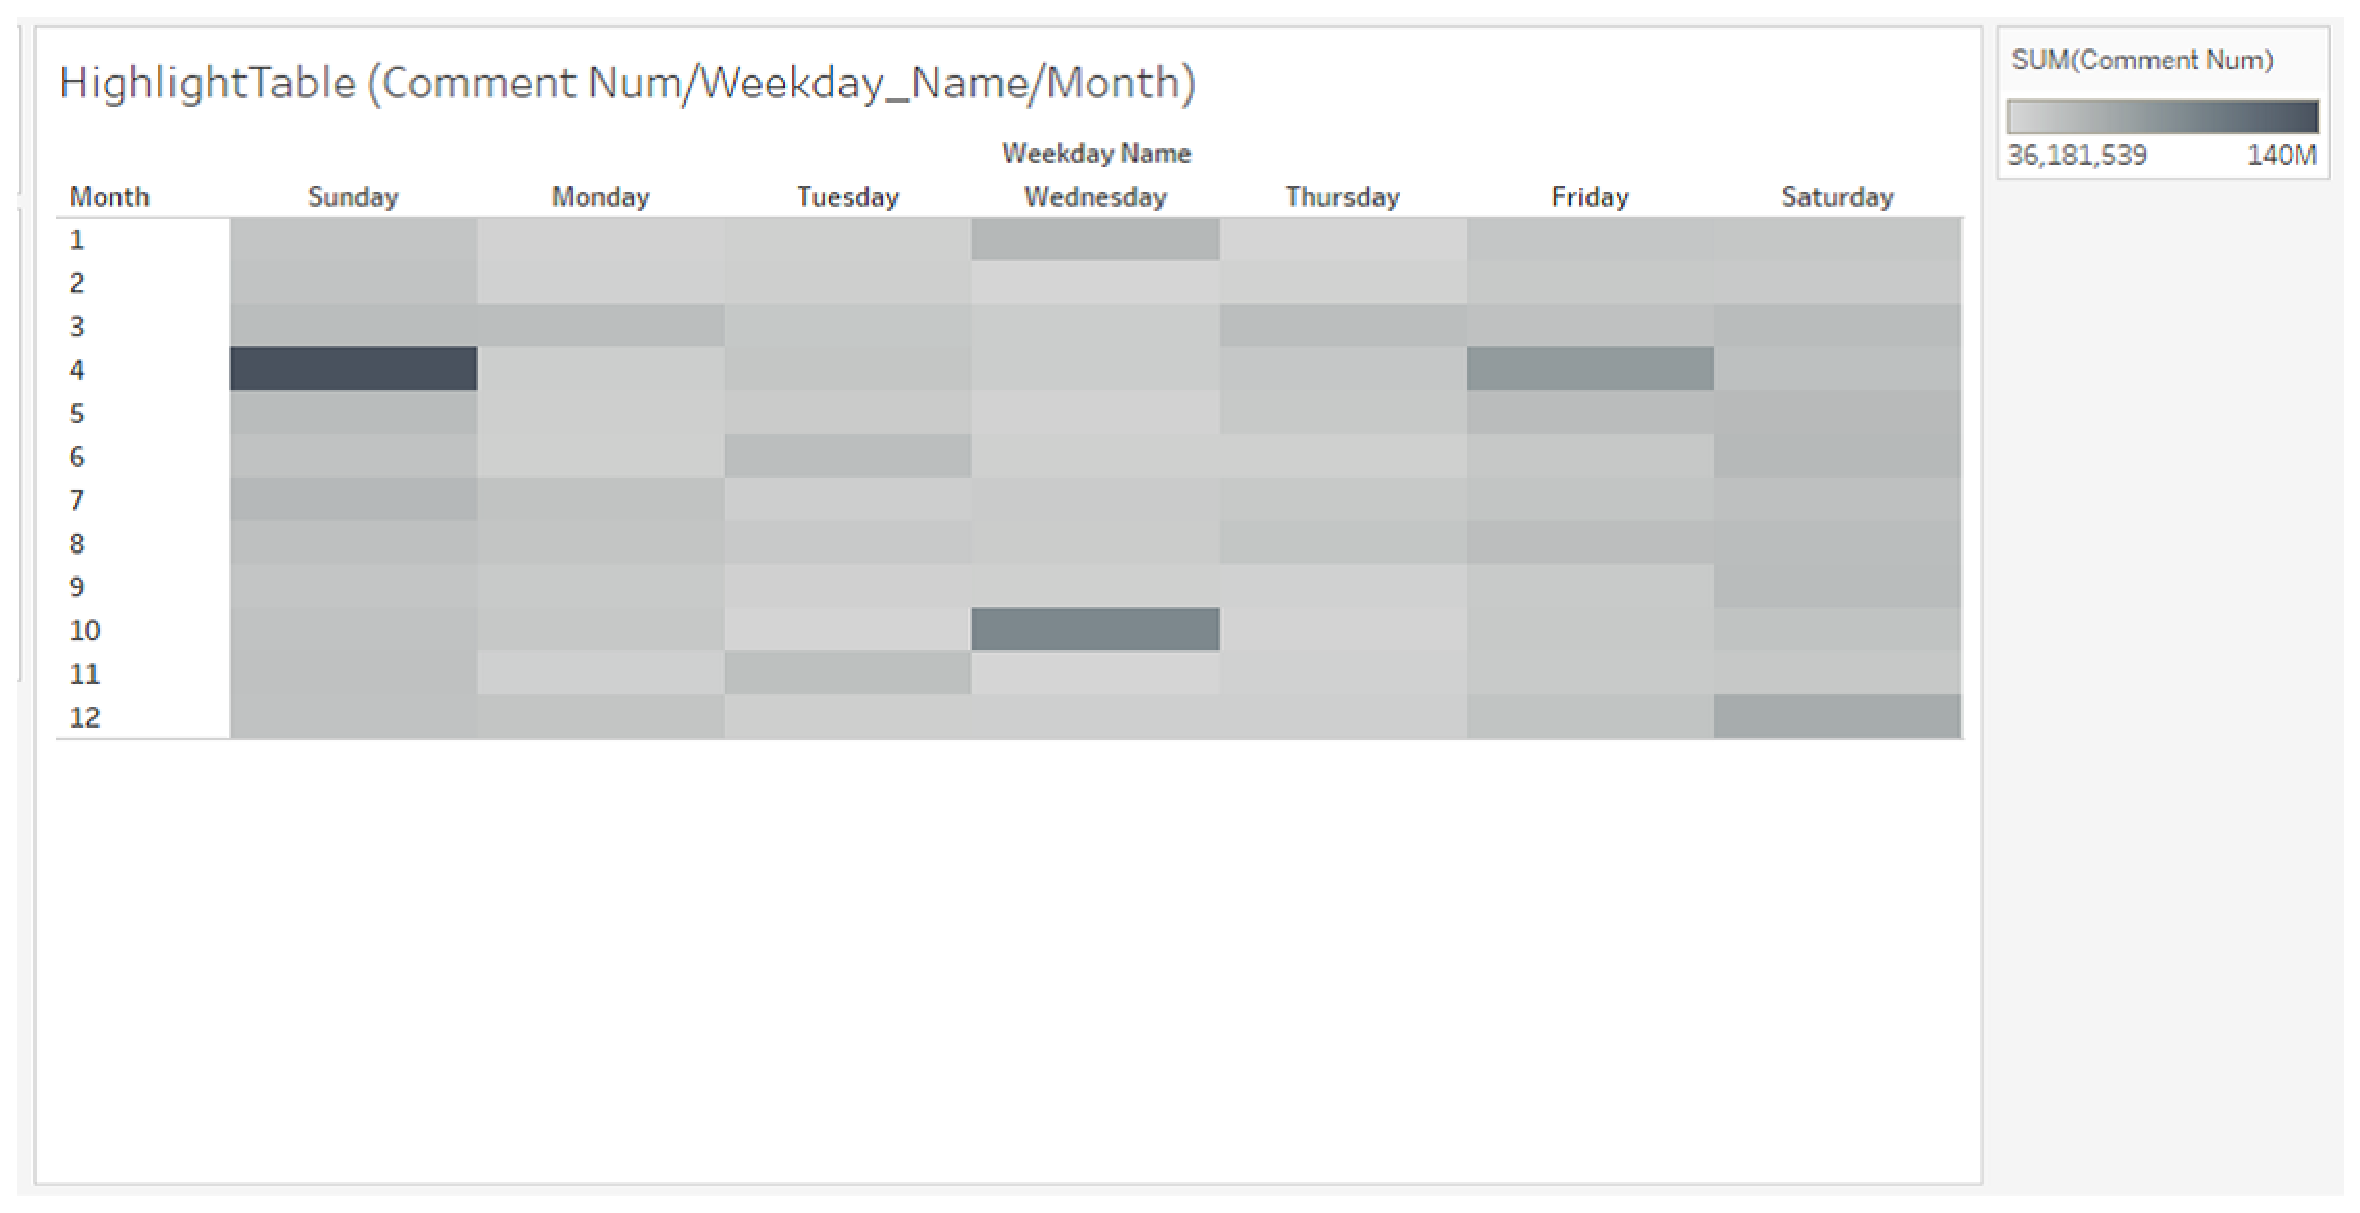
\includegraphics[width=\columnwidth]{./eps/HighlightTable_CommentNum_WeekdayNameMonth.eps}
    \subcaption{WeekdayName/Month}
    \label{fig:highlighttable_comment_num_weekdaynameMonth}
  \end{minipage}
  %
  \begin{minipage}[b]{0.49\columnwidth}
    \centering
    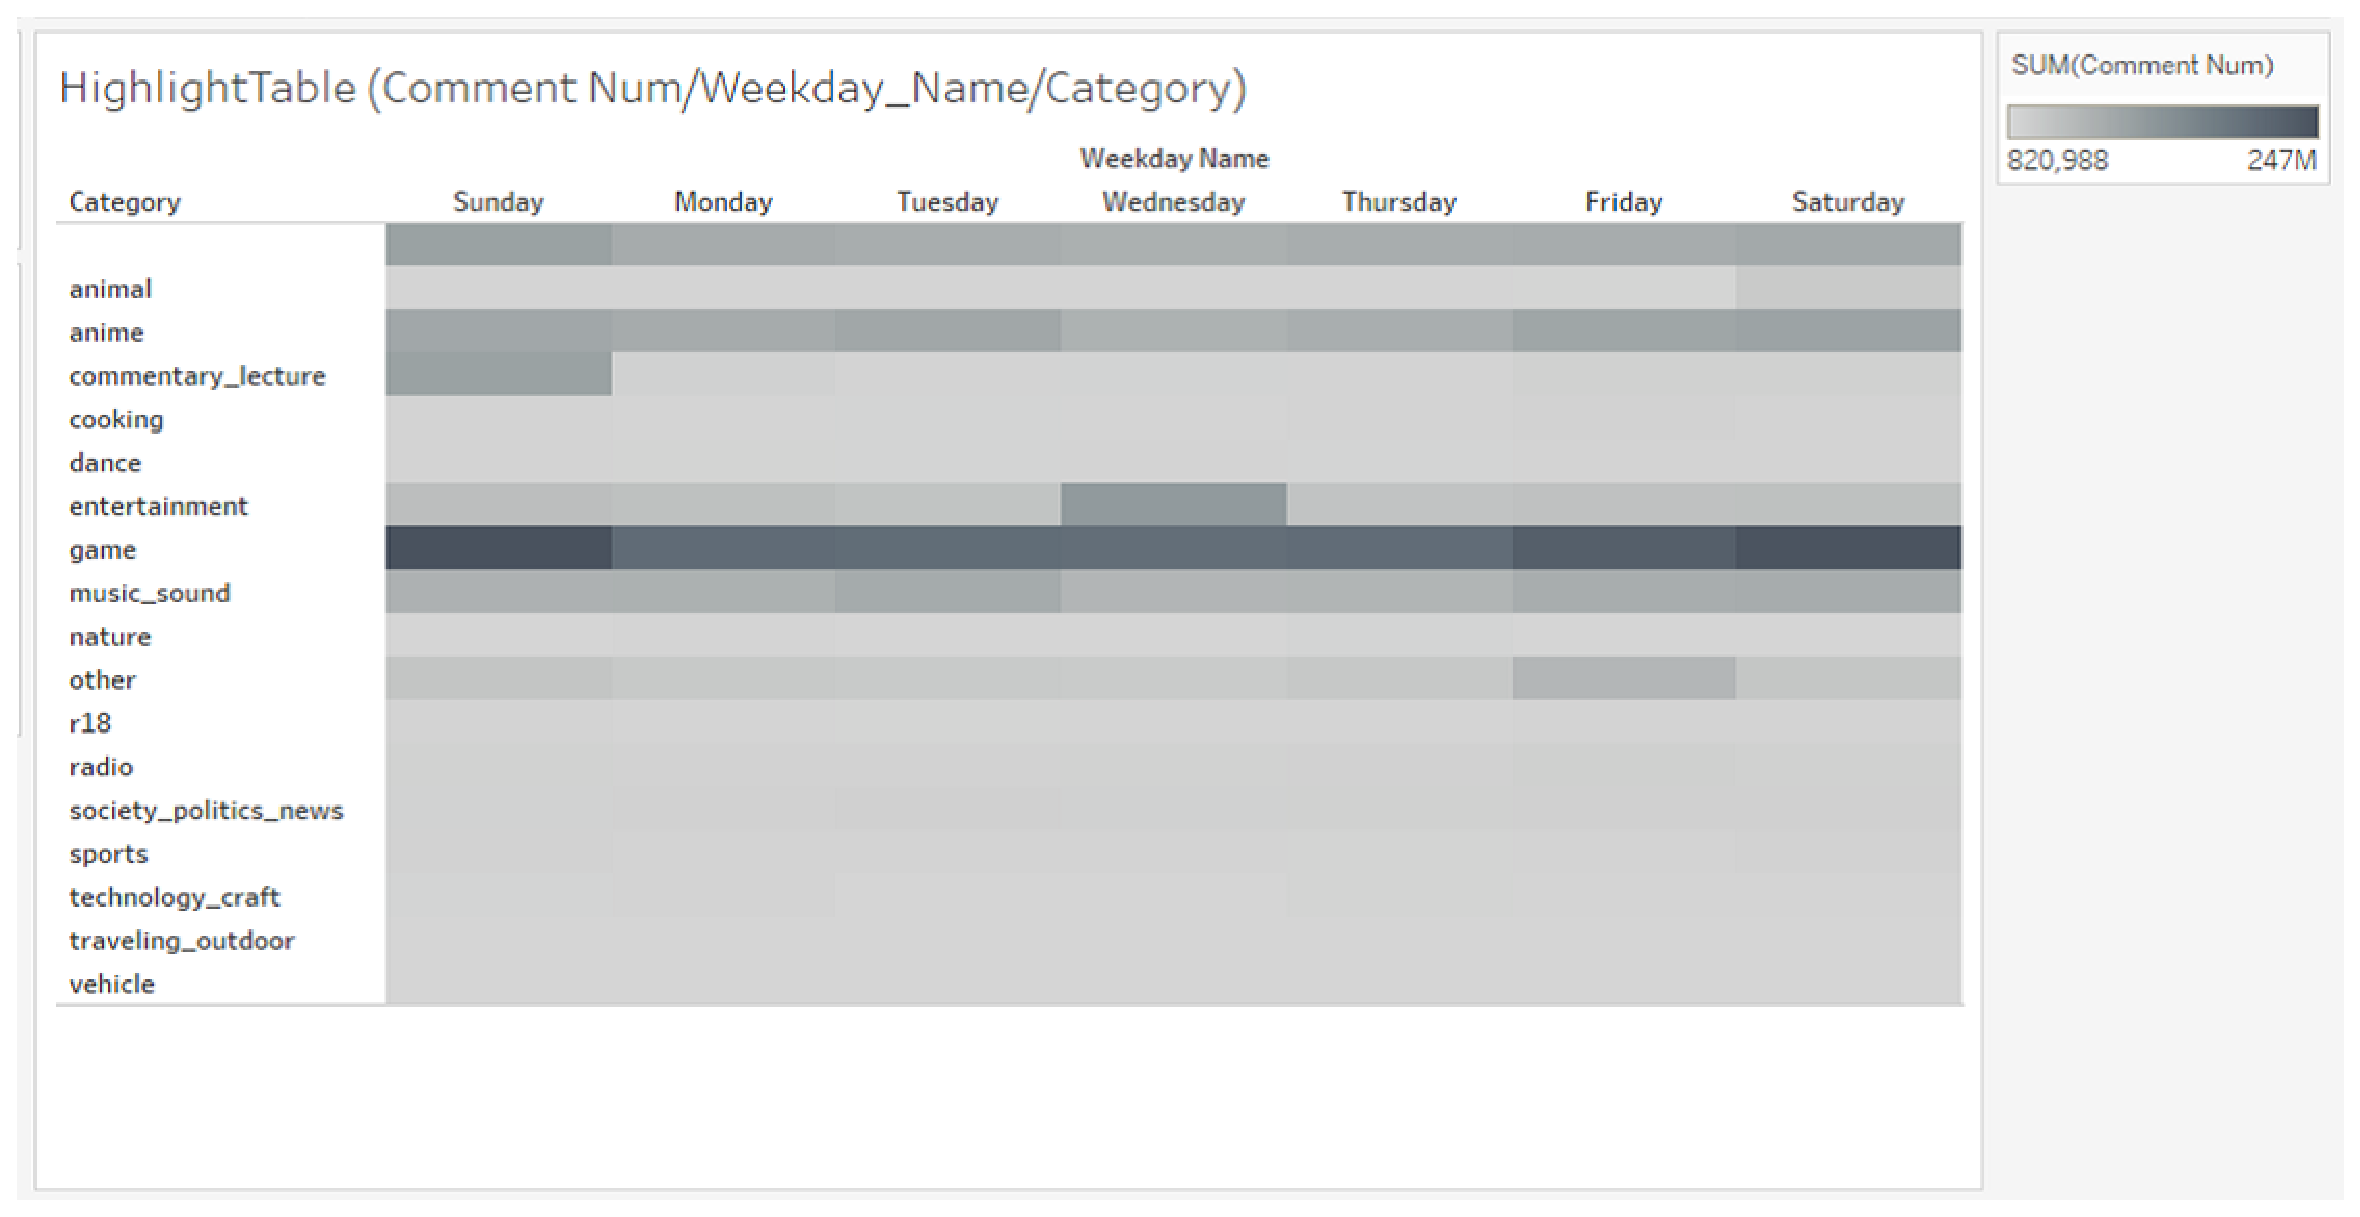
\includegraphics[width=\columnwidth]{./eps/HighlightTable_CommentNum_WeekdayNameCategory.eps}
    \subcaption{WeekdayName/Category}
    \label{fig:highlighttable_comment_num_weekdaynamecategory}
  \end{minipage}
  \vspace{-1.0zh}
  \caption{CommentNum(2)}
  \label{fig:highlighttable_comment_num_week}
  \vspace{-1.0zh}
\end{figure}


\newpage
\subsection{HighlightTable分析 - MylistNum}

マイリスト数を集計値として,可視化した結果を図\ref{fig:highlighttable_mylistnum_year}および
図\ref{fig:highlighttable_comment_num_week}に示す.
%
図\ref{fig:highlighttable_mylistnum_year}は縦軸が年であり,
横軸は時間,日,月,曜日の単位で集計している.
図\ref{fig:highlighttable_comment_num_week}は横軸が曜日であり,
縦軸は時間,日,月,カテゴリで集計している.

\vspace{-1.5zh}
\begin{figure}[h]
  \begin{minipage}[b]{0.49\columnwidth}
    \centering
    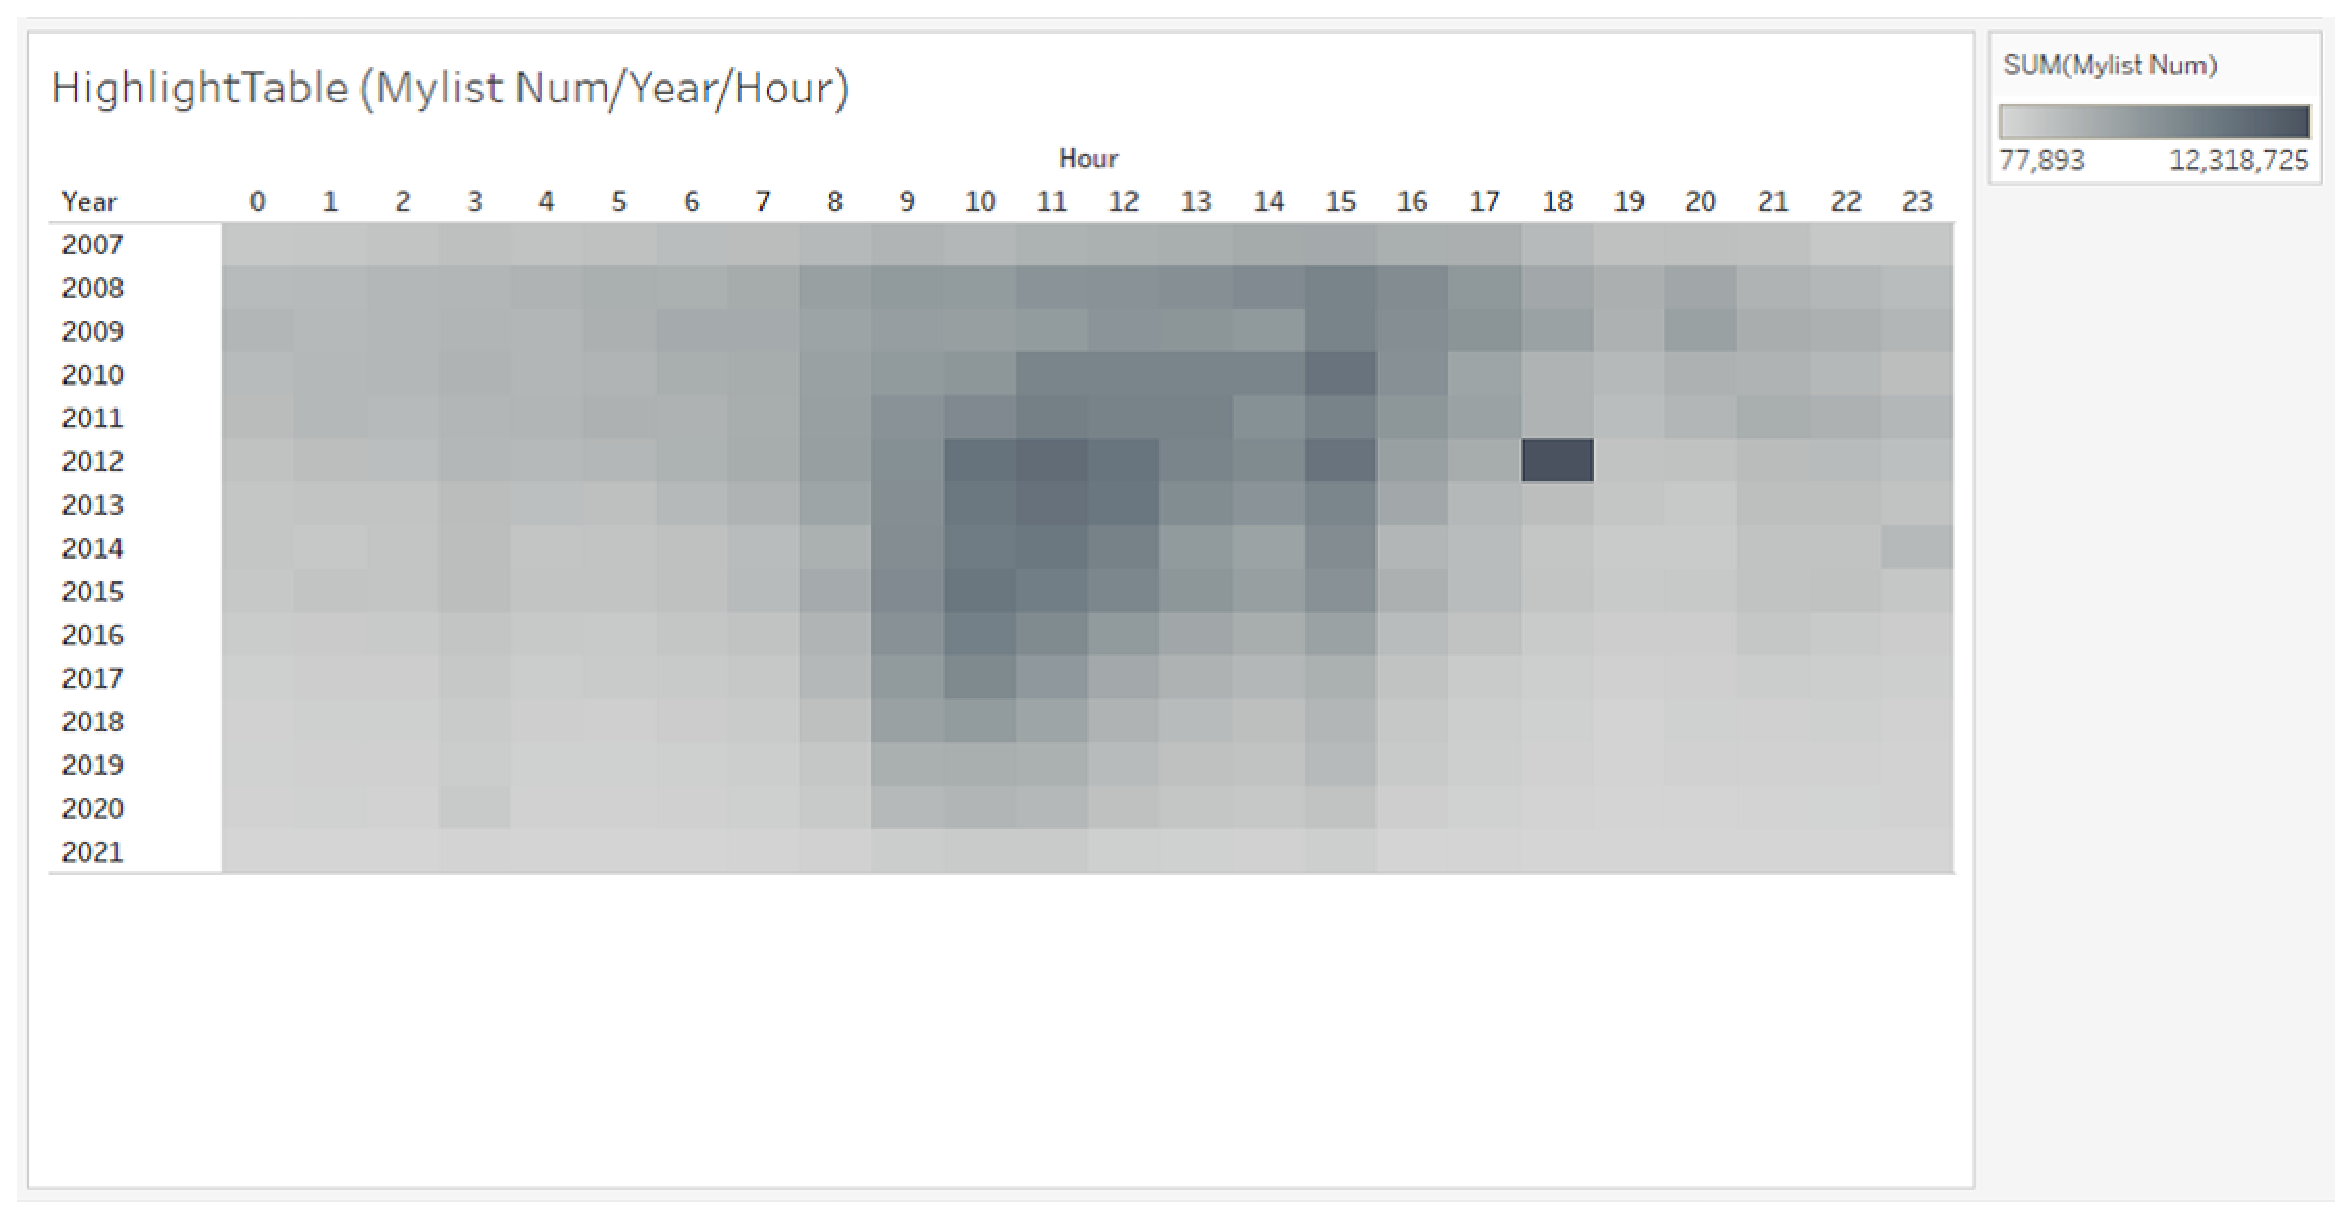
\includegraphics[width=\columnwidth]{./eps/HighlightTable_MylistNum_YearHour.eps}
    \subcaption{Year/Hour}
    \label{fig:highlighttable_mylistnum_yearhour}
  \end{minipage}
  %
  \begin{minipage}[b]{0.49\columnwidth}
    \centering
    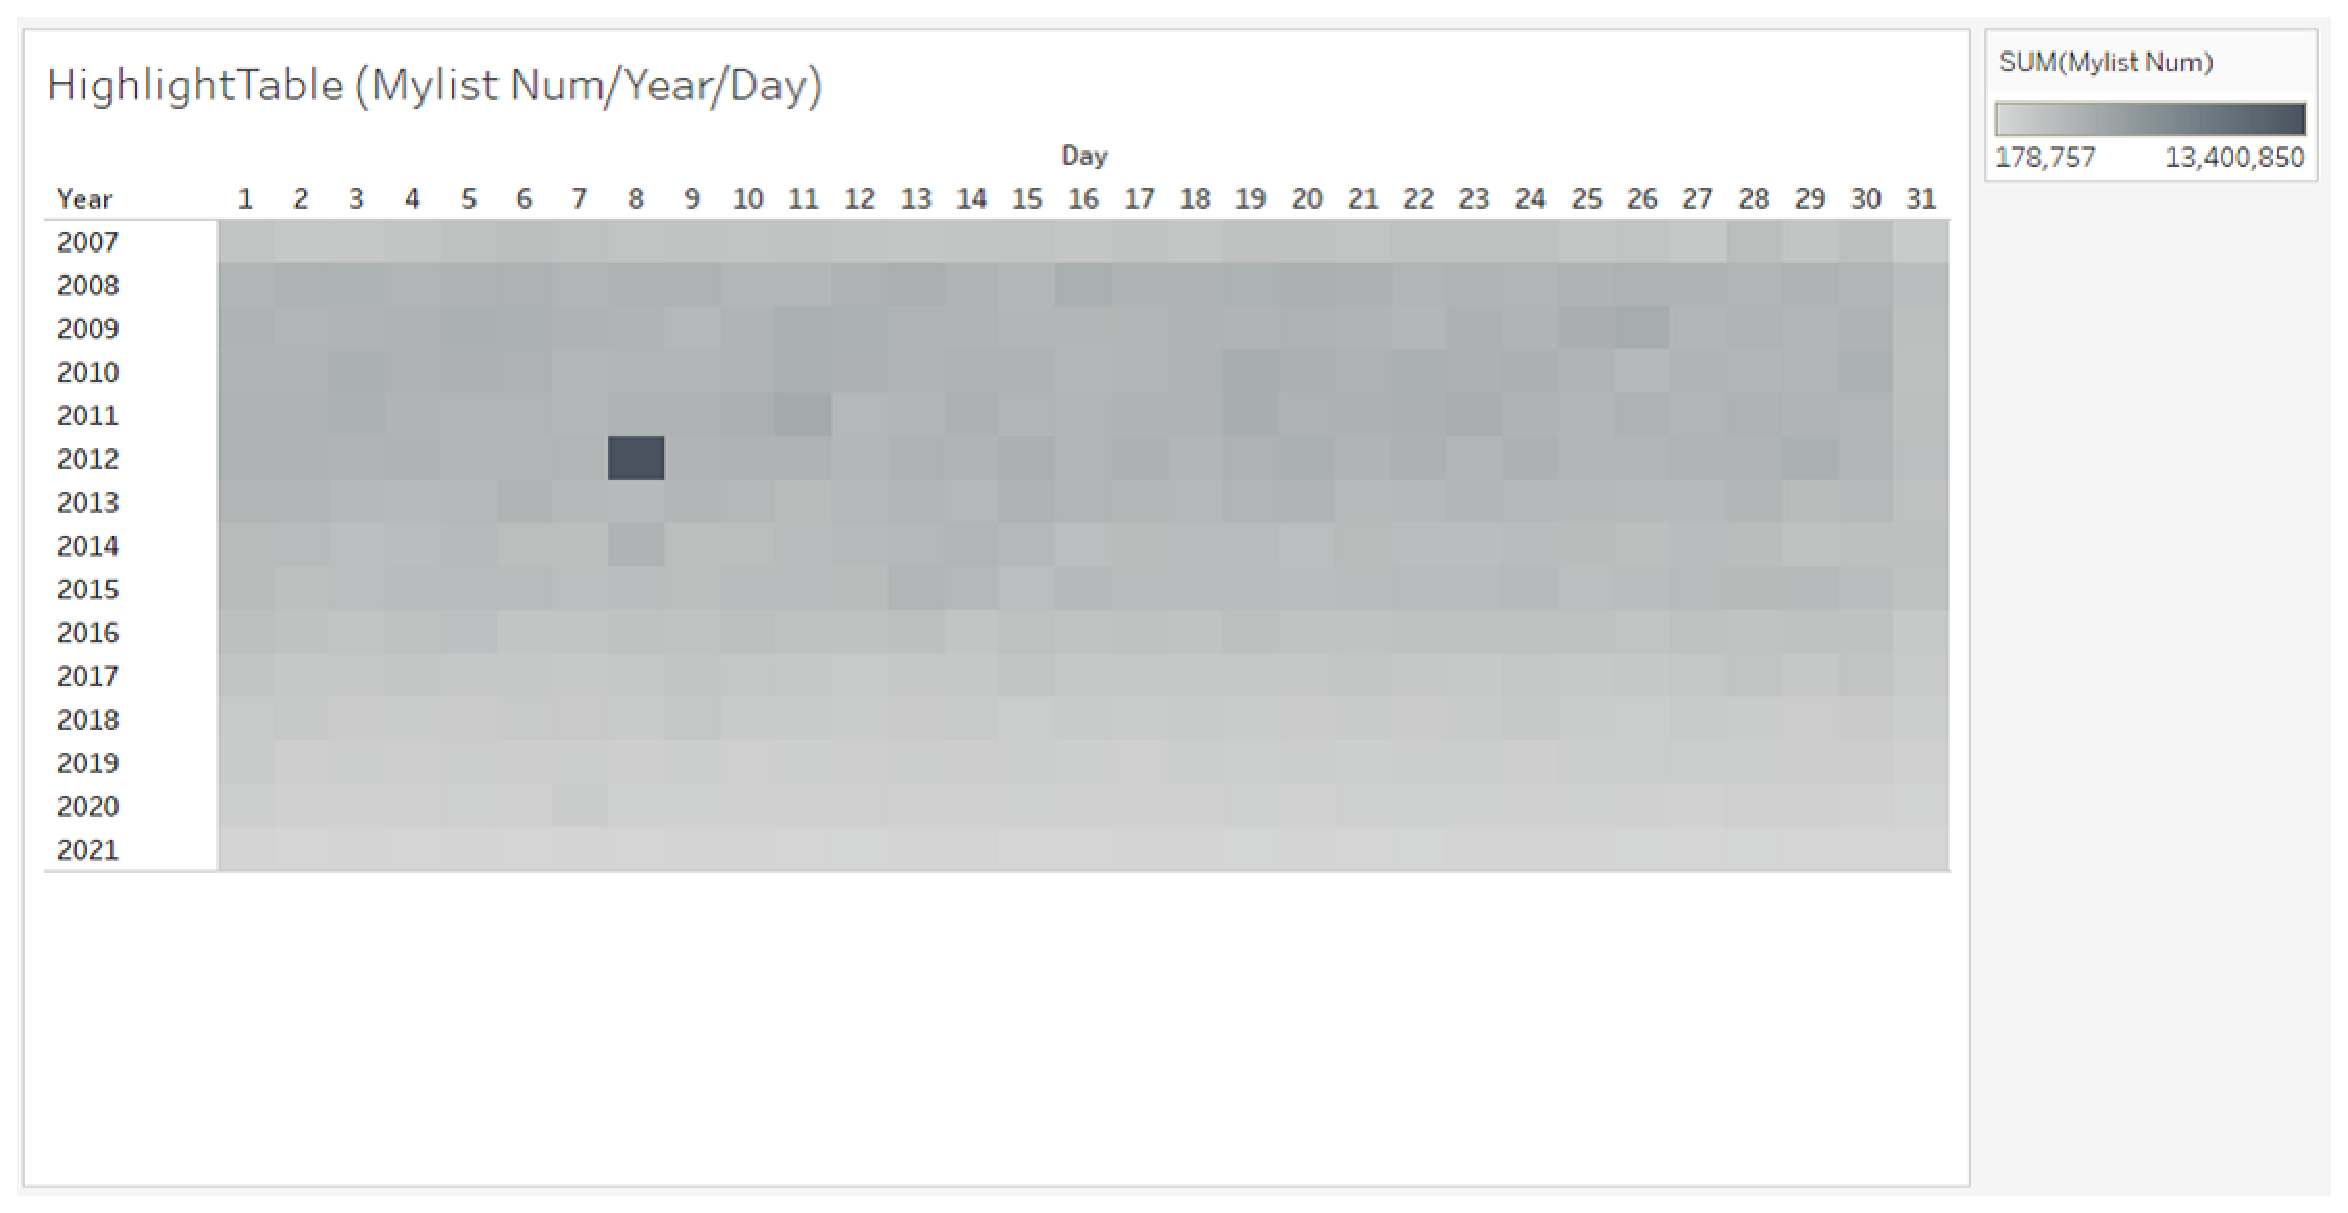
\includegraphics[width=\columnwidth]{./eps/HighlightTable_MylistNum_YearDay.eps}
    \subcaption{Year/Day}
    \label{fig:highlighttable_mylistnum_yearday}
  \end{minipage}
  %
  \begin{minipage}[b]{0.49\columnwidth}
    \centering
    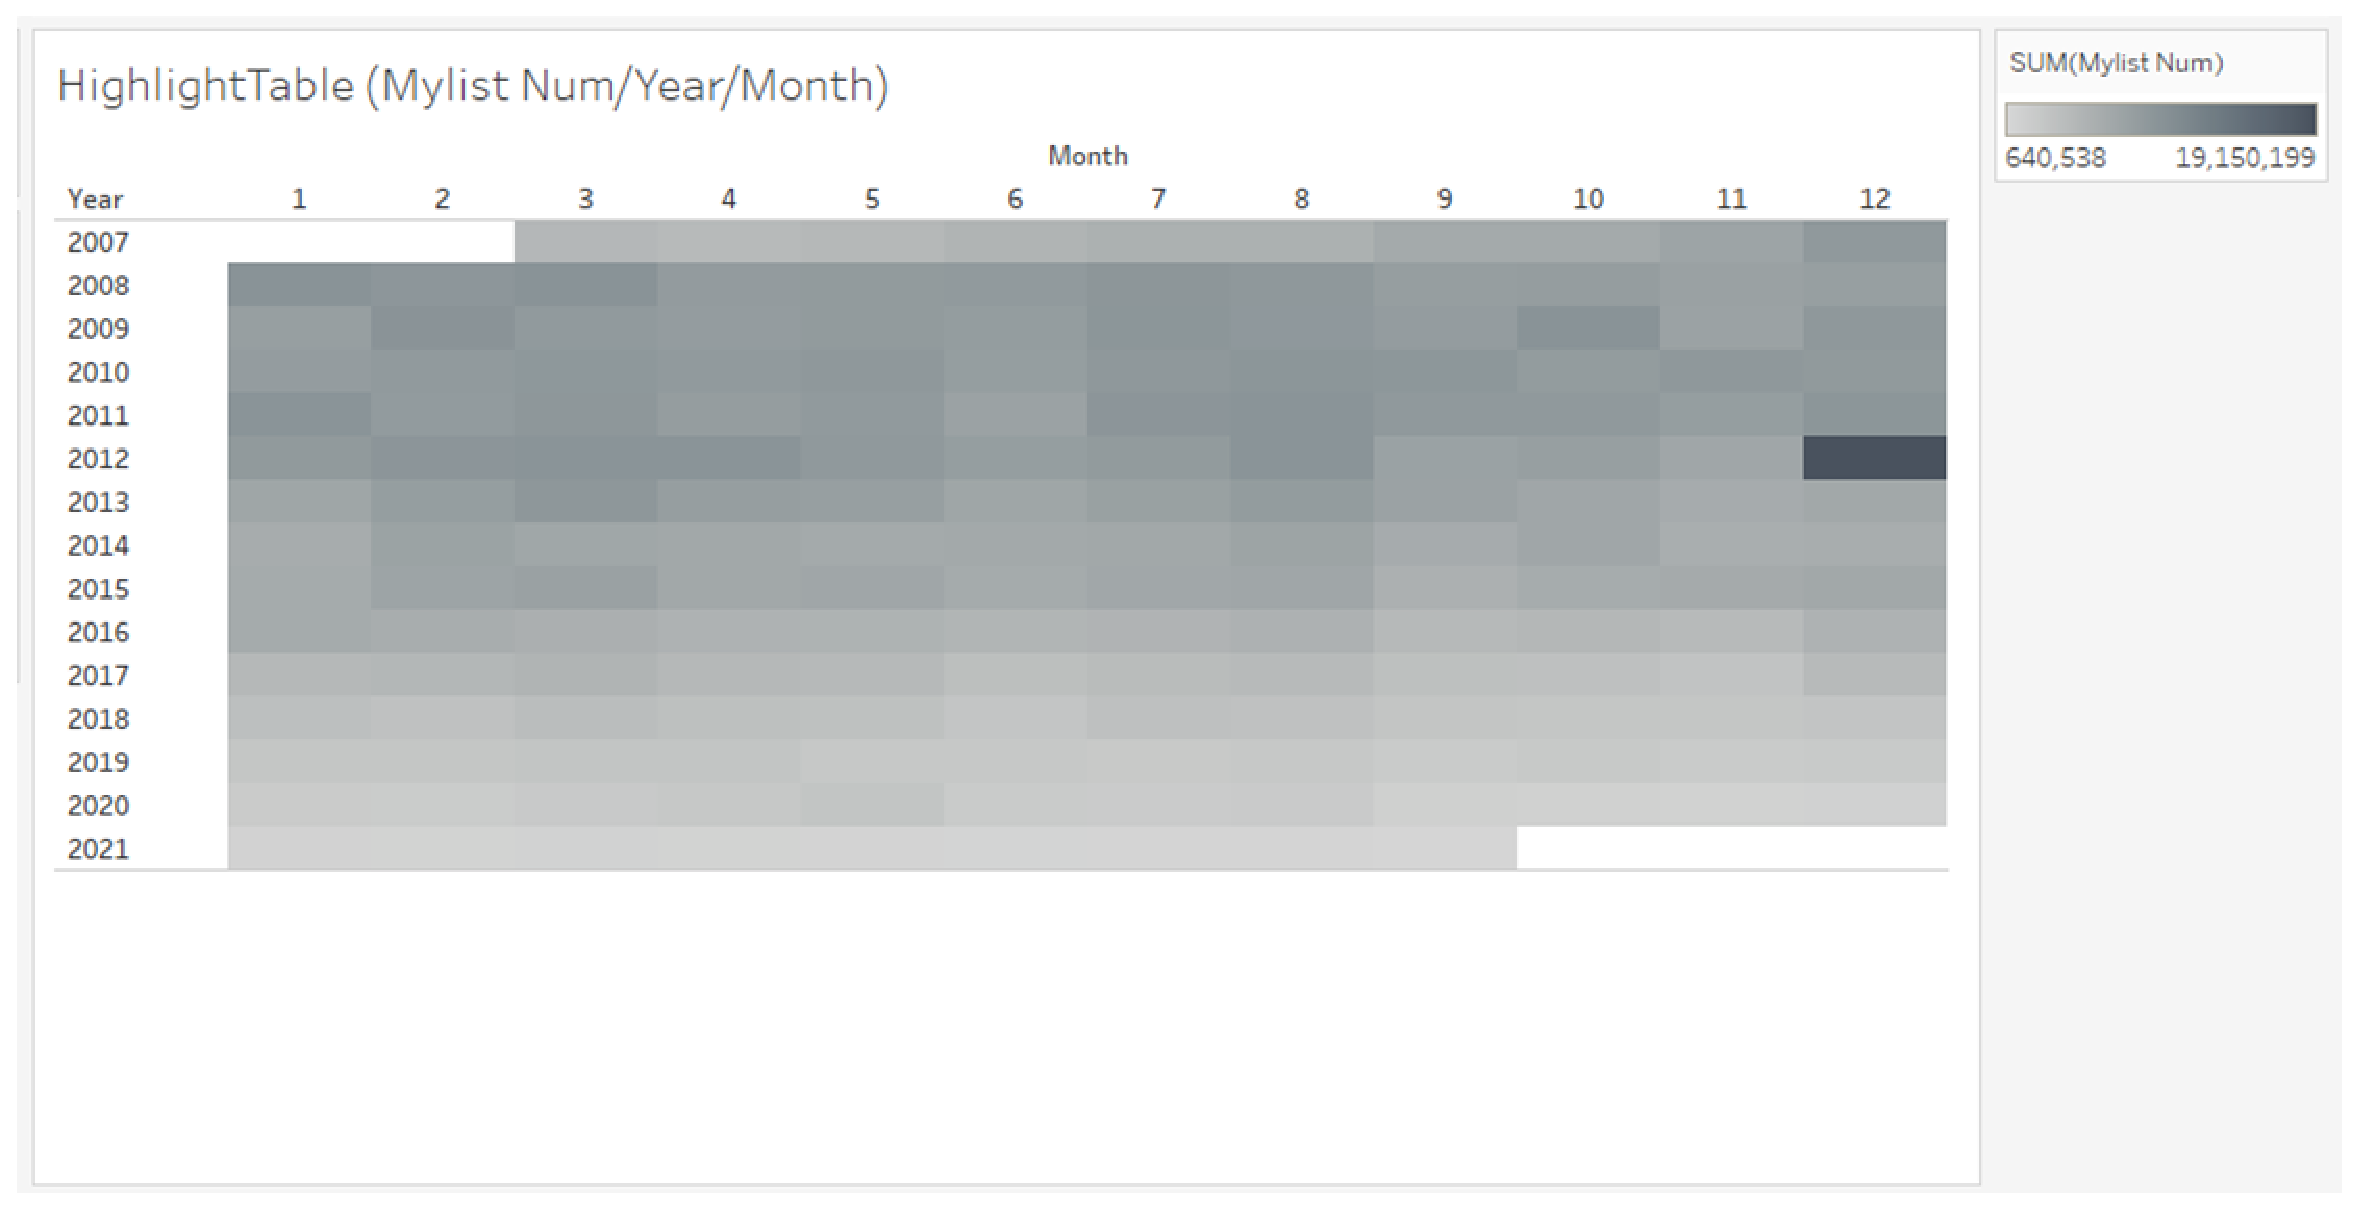
\includegraphics[width=\columnwidth]{./eps/HighlightTable_MylistNum_YearMonth.eps}
    \subcaption{Year/Month}
    \label{fig:highlighttable_mylistnum_yearmonth}
  \end{minipage}
  %
  \begin{minipage}[b]{0.49\columnwidth}
    \centering
    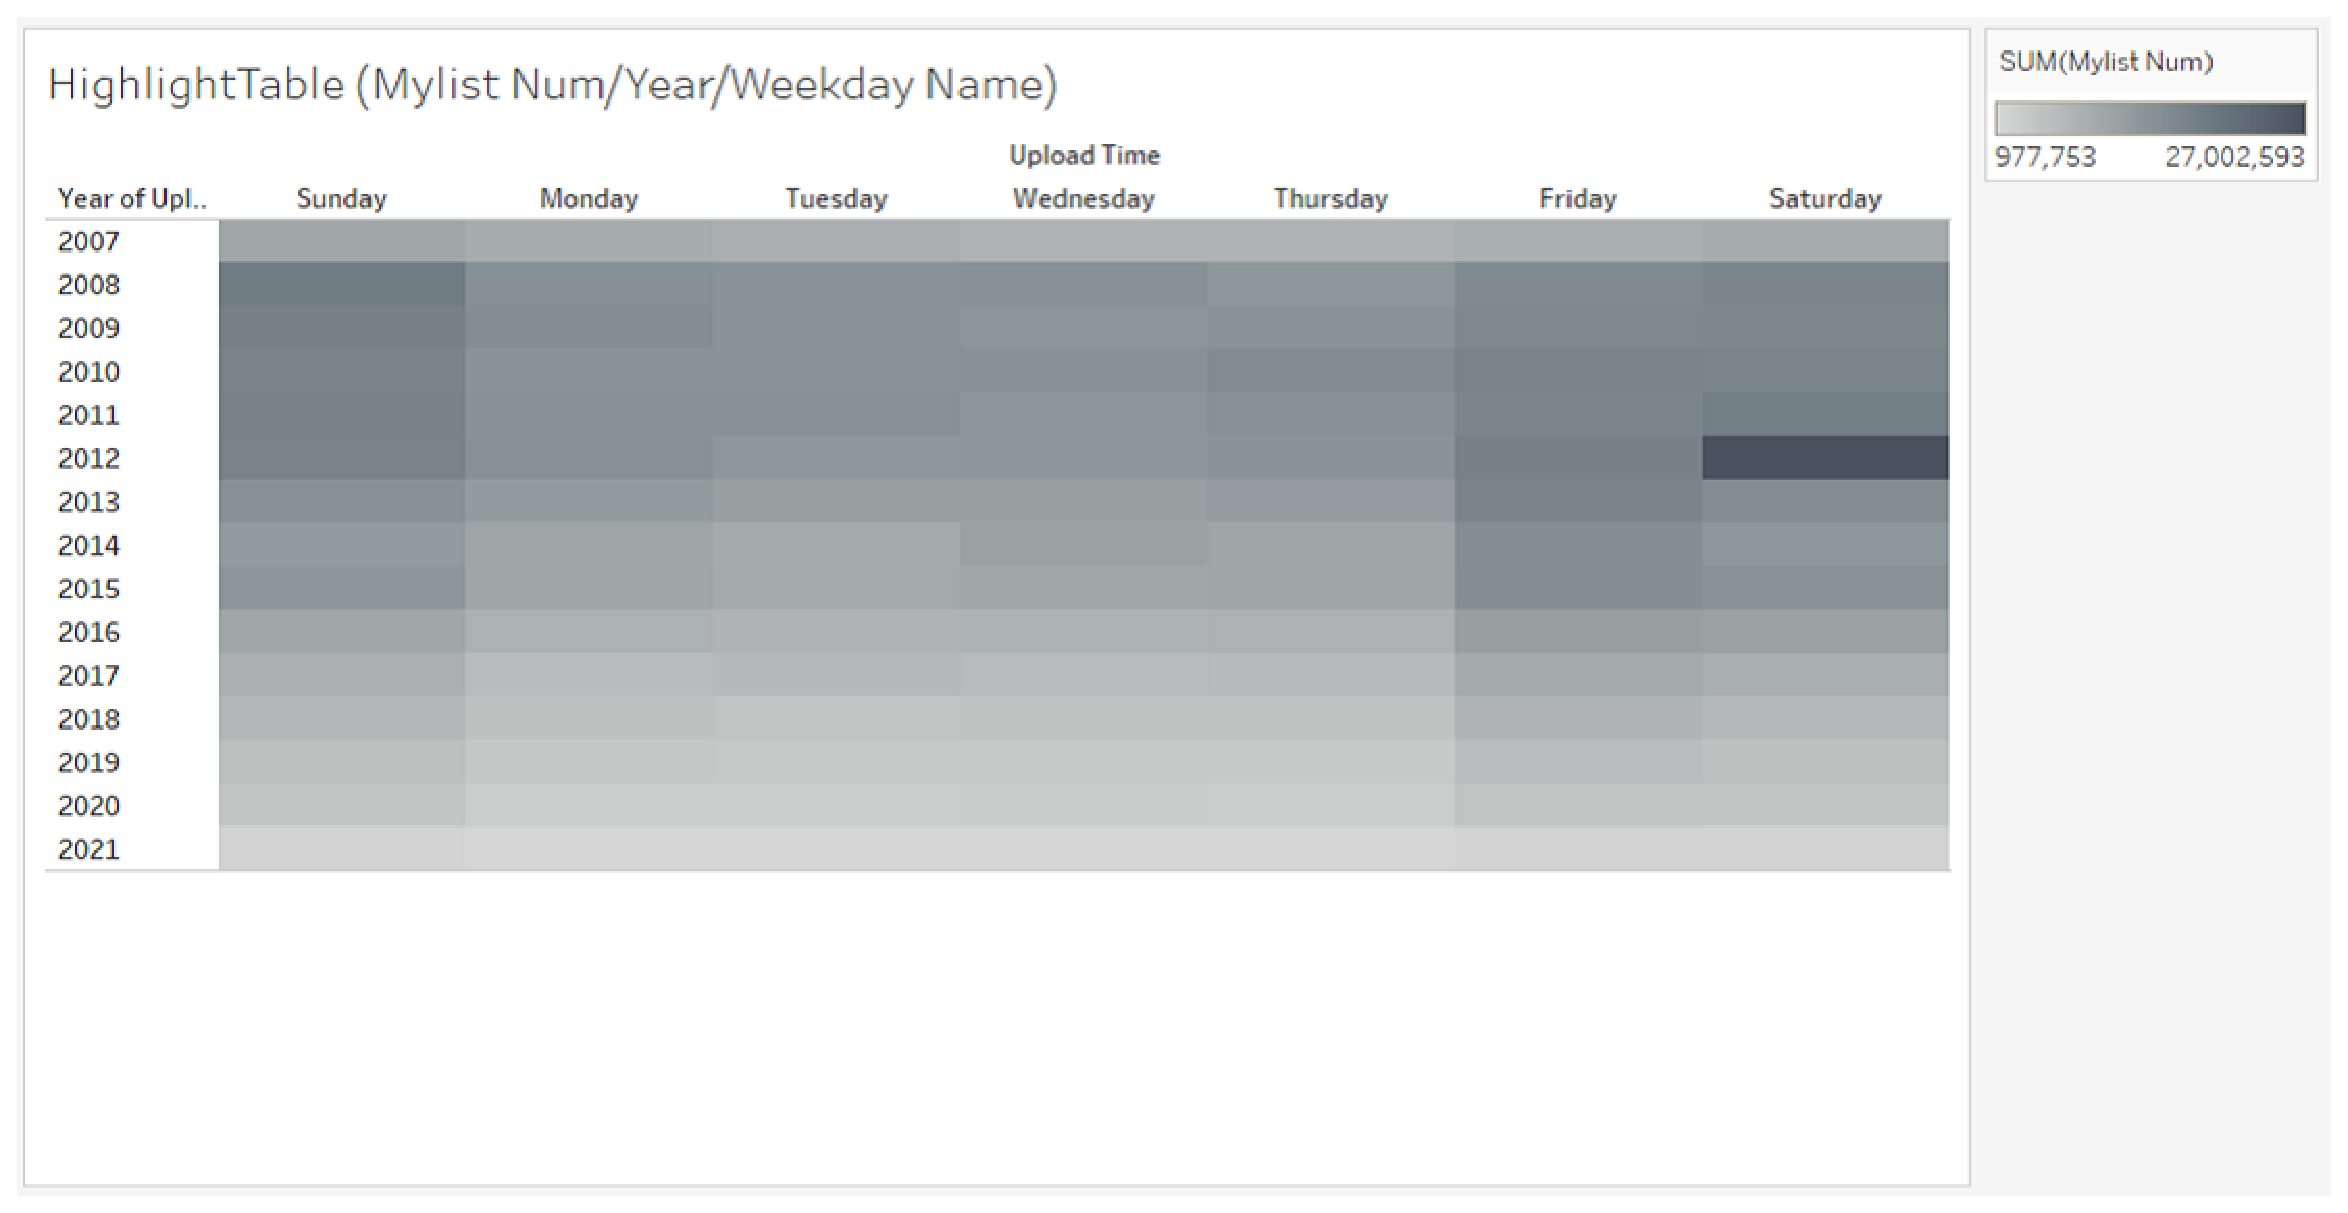
\includegraphics[width=\columnwidth]{./eps/HighlightTable_MylistNum_YearWeekdayName.eps}
    \subcaption{Year/WeekdayName}
    \label{fig:highlighttable_mylistnum_yearweekdayname}
  \end{minipage}
  \vspace{-1.0zh}
  \caption{MylistNum(1)}
  \vspace{-1.0zh}
    \label{fig:highlighttable_mylist_year}
\end{figure}
%
\vspace{-2.5zh}
%
\begin{figure}[h]
  \hspace{-1.0zh}
  \begin{minipage}[b]{0.49\columnwidth}
    \centering
    \hspace{-1.0zh}
    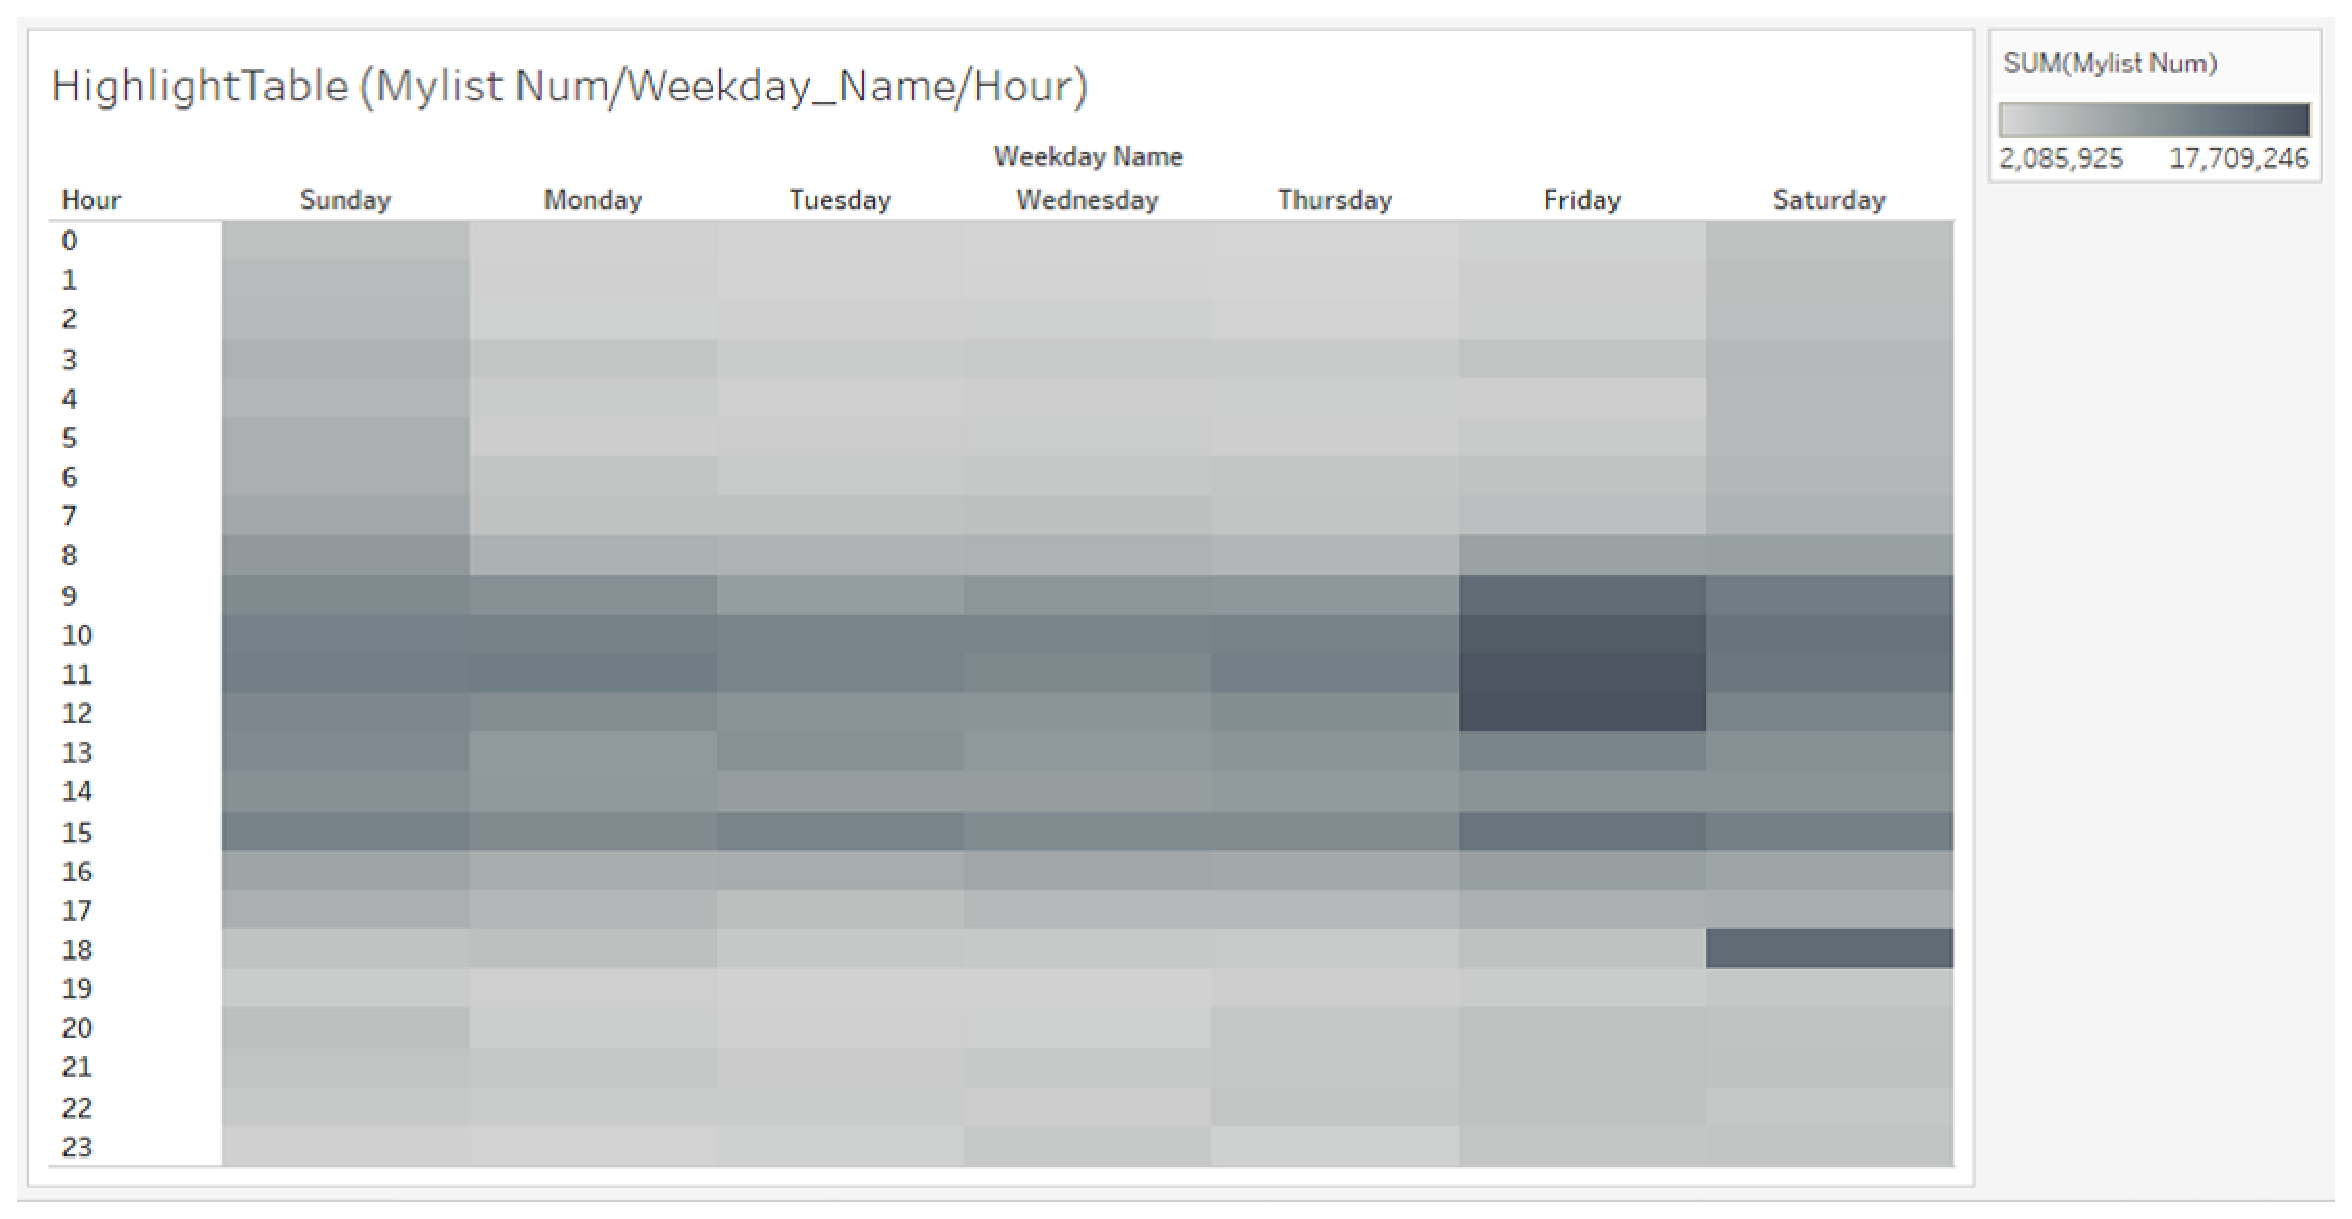
\includegraphics[width=\columnwidth]{./eps/HighlightTable_MylistNum_WeekdayNameHour.eps}
    \subcaption{WeekdayName/Hour}
    \label{fig:highlighttable_mylist_weekdaynamehour}
  \end{minipage}
  %
  \begin{minipage}[b]{0.49\columnwidth}
    \centering
    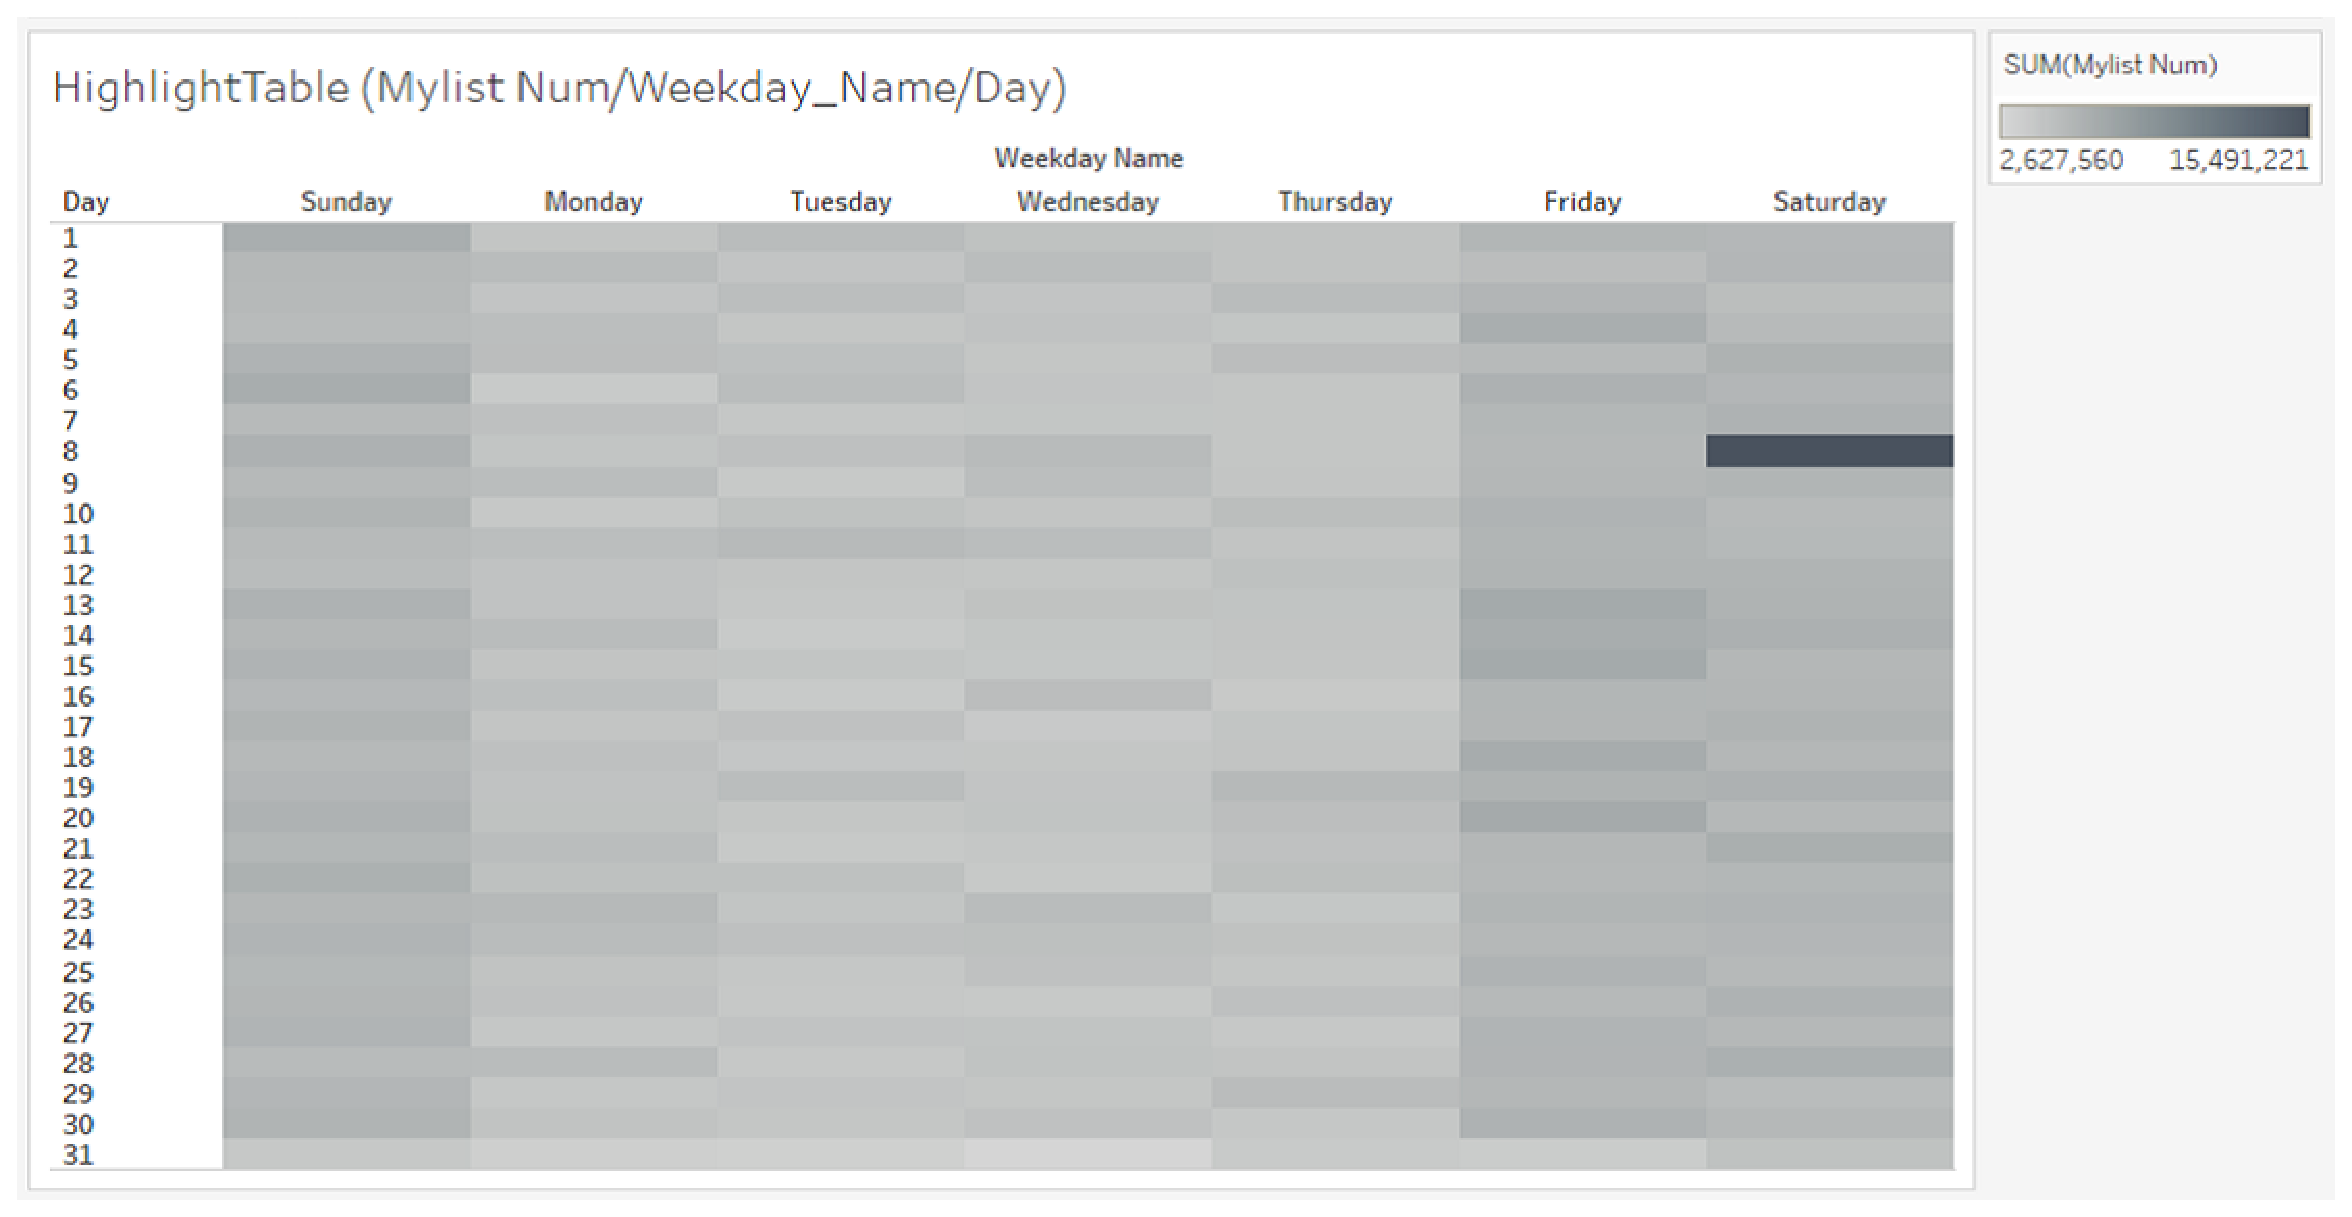
\includegraphics[width=\columnwidth]{./eps/HighlightTable_MylistNum_WeekdayNameDay.eps}
    \subcaption{WeekdayName/Day}
    \label{fig:highlighttable_mylist_weekdaynameday}
  \end{minipage}
  %
  \begin{minipage}[b]{0.49\columnwidth}
    \centering
    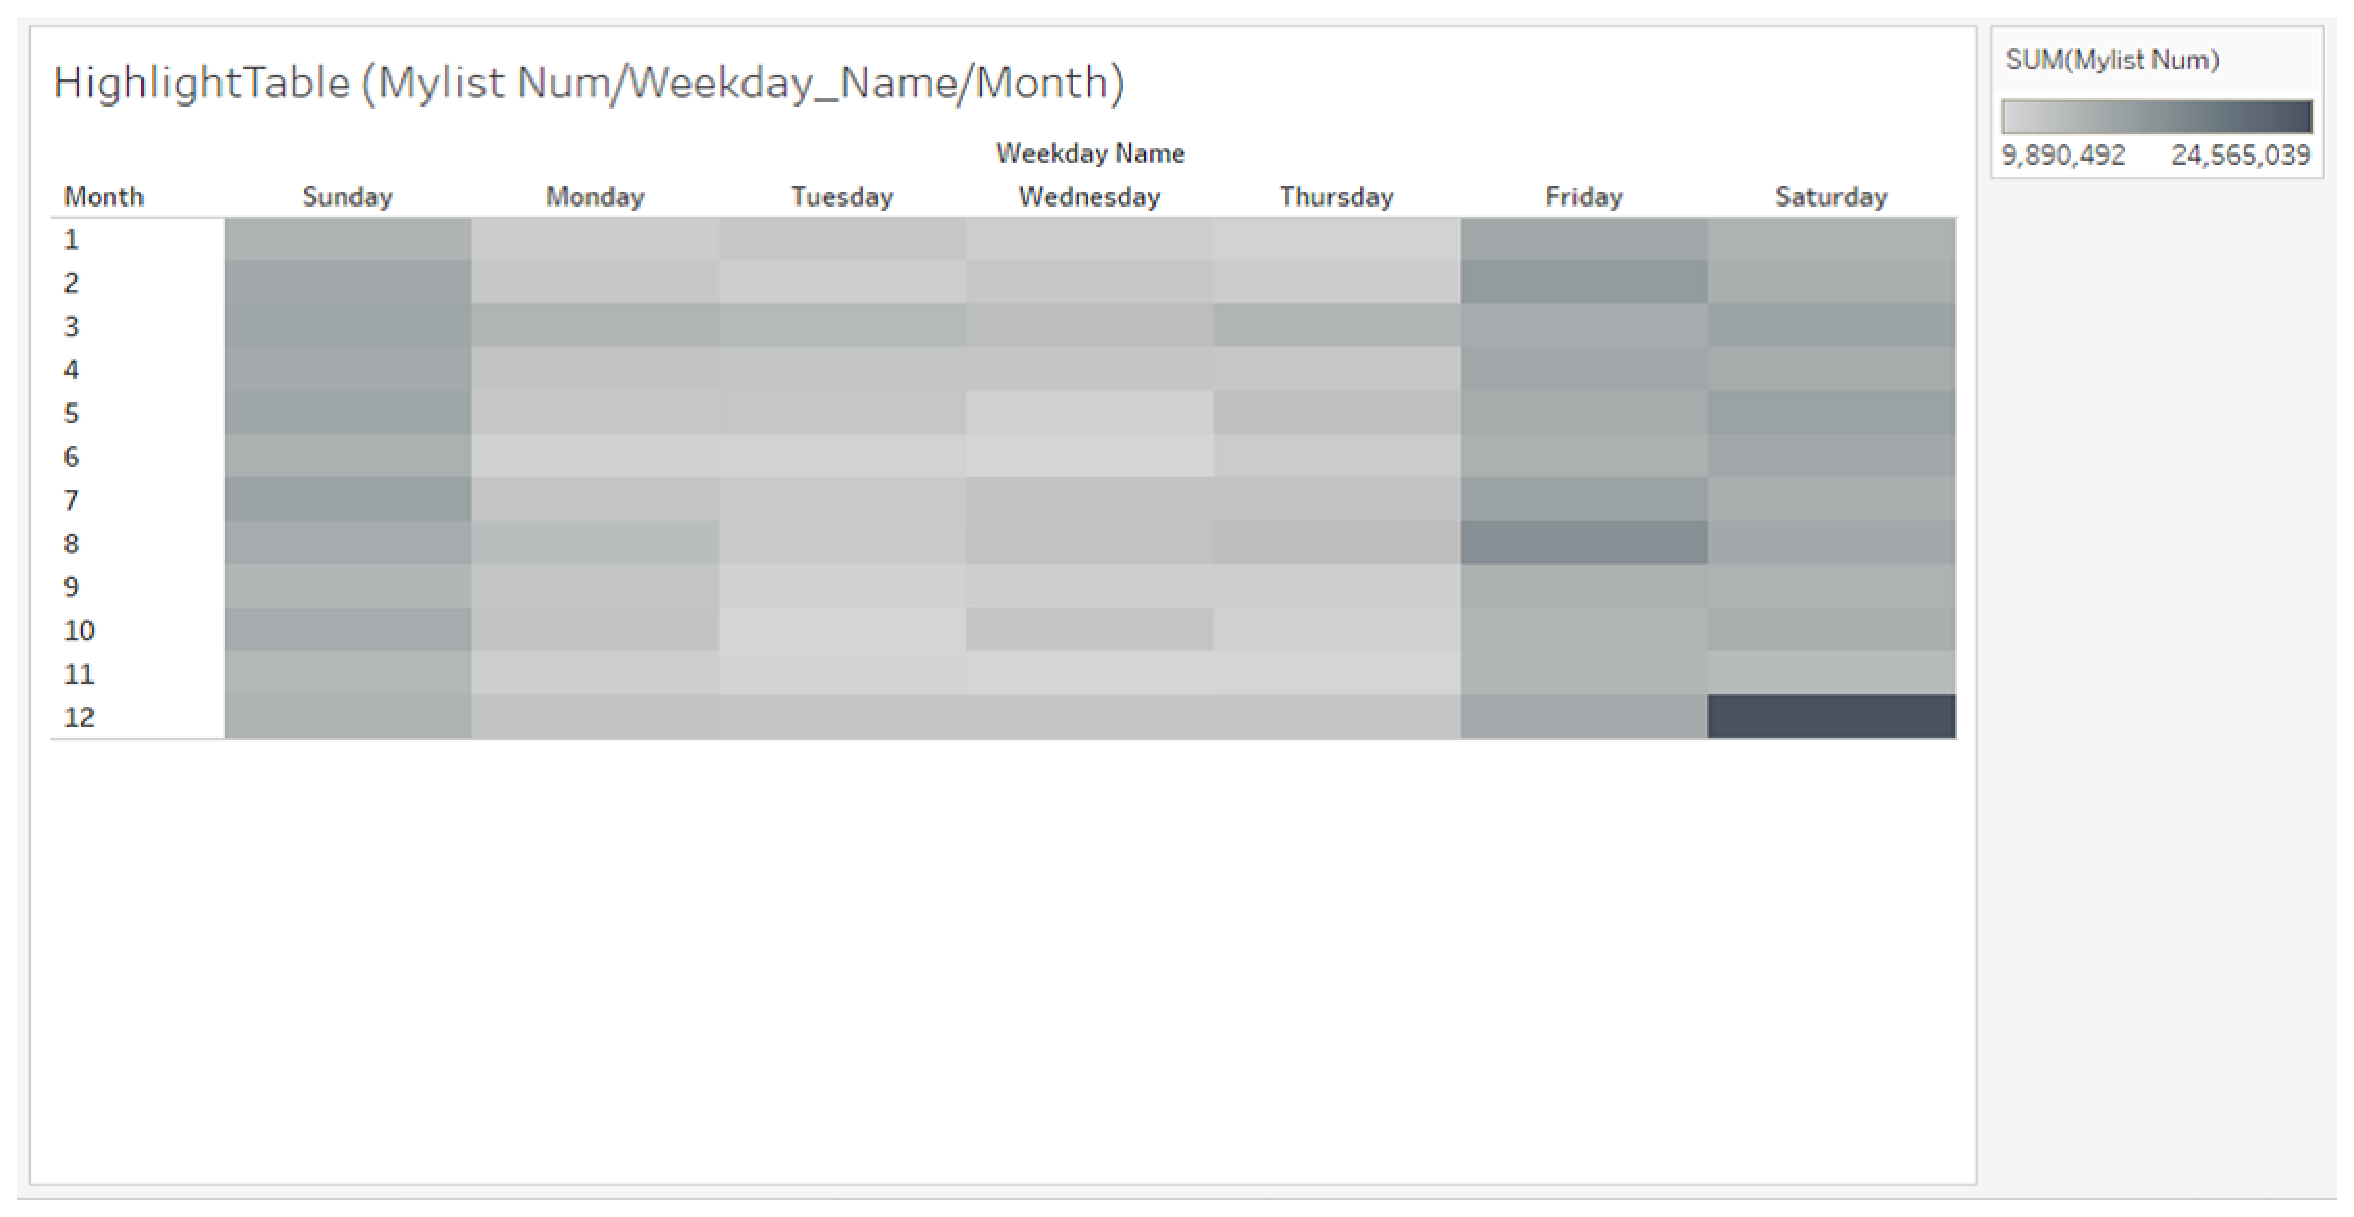
\includegraphics[width=\columnwidth]{./eps/HighlightTable_MylistNum_WeekdayNameMonth.eps}
    \subcaption{WeekdayName/Month}
    \label{fig:highlighttable_mylist_weekdaynamemonth}
  \end{minipage}
  %
  \begin{minipage}[b]{0.49\columnwidth}
    \centering
    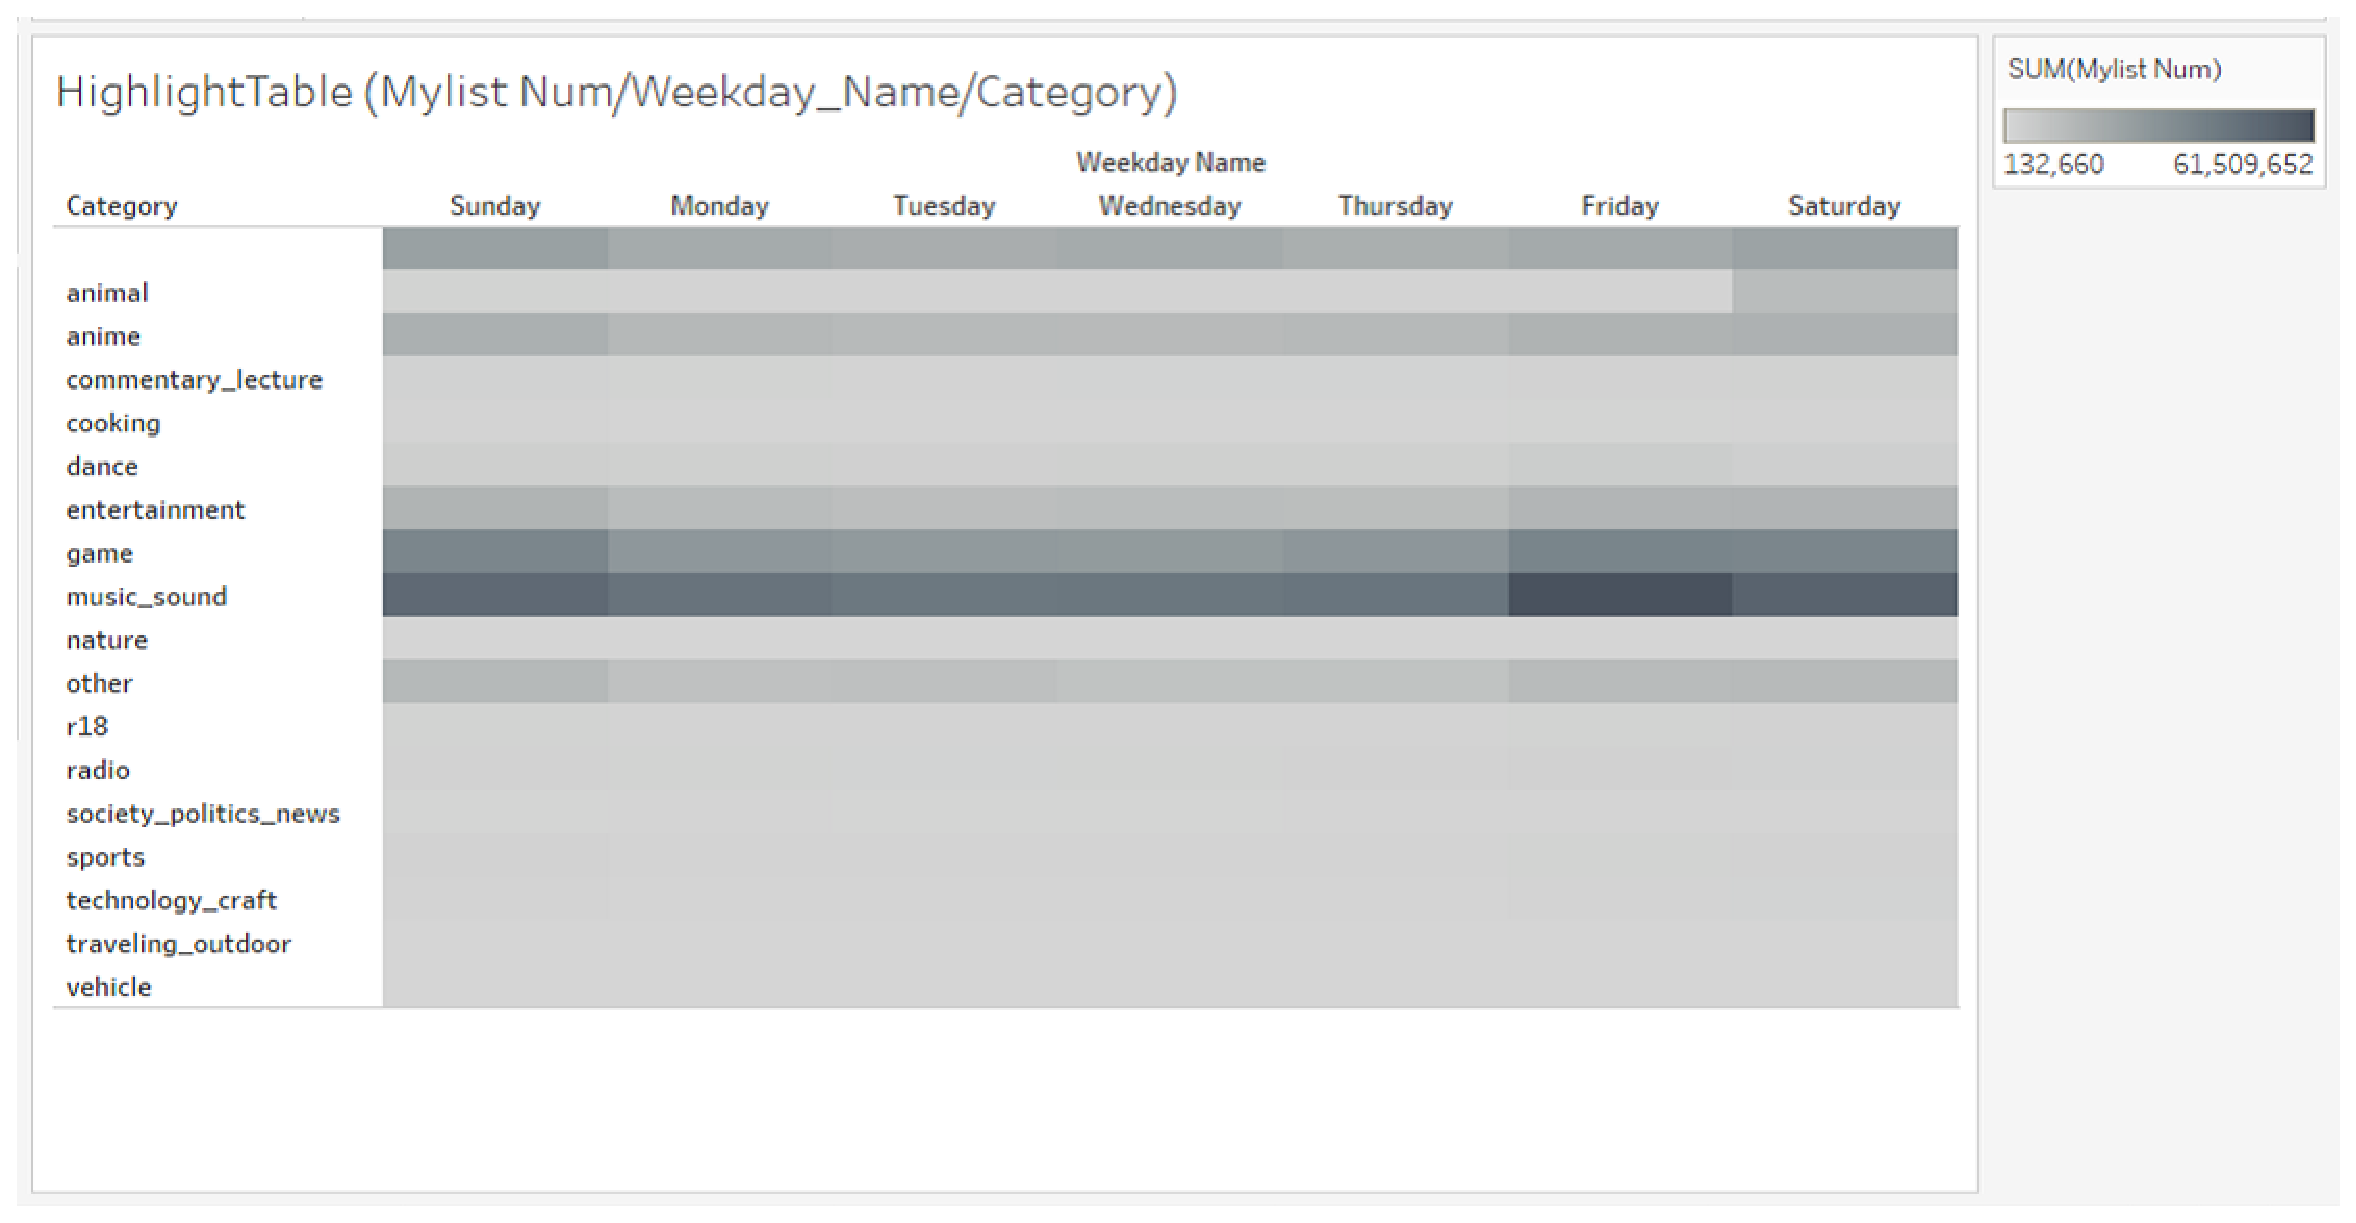
\includegraphics[width=\columnwidth]{./eps/HighlightTable_MylistNum_WeekdayNameCategory.eps}
    \subcaption{WeekdayName/Category}
    \label{fig:highlighttable_mylist_weekdaynamecategory}
  \end{minipage}
  \vspace{-1.0zh}
  \caption{MylistNum(2)}
  \label{fig:highlighttable_mylist_numweekday}
  \vspace{-1.0zh}
\end{figure}


\newpage


\section{まとめ}





%4.6.3
\section*{謝辞}
本研究では,国立情報学研究所のIDRデータセット提供サービスにより
株式会社ドワンゴから提供を受けた「ニコニコ動画コメント等データ」を利用した.
ここに記してデータ提供頂いた株式会社ドワンゴに感謝申し上げます.\\


\bibliographystyle{junsrt}
\bibliography{ipsj_bibliography}


\end{document}
